\begin{document}

% Front matter
\frontmatter

%% r.1 blank page
%\blankpage
%
%% v.2 epigraphs
%\newpage\thispagestyle{empty}
%\openepigraph{%
%The public is more familiar with bad design than good design.
%It is, in effect, conditioned to prefer bad design, 
%because that is what it lives with. 
%The new becomes threatening, the old reassuring.
%}{Paul Rand%, {\itshape Design, Form, and Chaos}
%}
%\vfill
%\openepigraph{%
%A designer knows that he has achieved perfection 
%not when there is nothing left to add, 
%but when there is nothing left to take away.
%}{Antoine de Saint-Exup\'{e}ry}
%\vfill
%\openepigraph{%
%The designer of a new system must not only be the implementor and the first 
%large-scale user; the designer should also write the first user manual\ldots 
%If I had not participated fully in all these activities, 
%literally hundreds of improvements would never have been made, 
%because I would never have thought of them or perceived 
%why they were important.
%}{Donald E. Knuth}


% r.3 full title page
\maketitle

%\addcontentsline{toc}{chapter}{Front Matter }

% v.4 copyright page
\newpage
\begin{fullwidth}
%    \addcontentsline{toc}{chapter}{Abstract and Bibliographic Information}%
	{\large {\it Authors\ \ } Vic Smith, Laith Alissa, Jon Cave, Joseph Siddall
	
	\vspace{1em}\noindent{\it Supervisor\ \ } Sara Kalvala
	
	\vspace{1em}\noindent{\it Abstract\ \ } A full multiplayer strategy game --- designed to be competitive in the current independent game market --- was developed and implemented exclusively using the Haskell language, with the goal of evaluating the efficacy of Haskell for development of this nature. Haskell was shown to be quite effective in this space, despite the pure functional nature of the language and the comparative lack of library support in the domain of games. Full details of the strengths and challenges of this approach are reported on herein, and a set of best practices for the use of Haskell in games development are suggested.
	
	\vspace{1em}\noindent{\it Keywords\ \ } Functional Programming, Haskell, Game Development, Graphical User Interface, Networking
	
	}
	
	~\vfill
	\thispagestyle{empty}
	\setlength{\parindent}{0pt}
	\setlength{\parskip}{\baselineskip}
	Copyright \copyright\ \the\year\ \plainauthor
	
	\par\smallcaps{Published by \newlinetospace{\thanklesspublisher}}
	
	%\par\smallcaps{Typesetting: tufte-latex.googlecode.com}
	
	\par\textit{First printing, \monthyear}

	\newpage

\end{fullwidth}

% Dedication
~\vfill
\begin{doublespace}
\noindent\fontsize{18}{22}\selectfont\itshape
\nohyphenation
Dedicated to the Haskell Community, upon whose shoulders rest this and many other projects.
\end{doublespace}
\vfill
\vfill


\begin{fullwidth}

\cleardoublepage

% Contents
%\addcontentsline{toc}{chapter}{Detailed Contents, Lists of Figures, Tables, and Listings}
\tableofcontents

\cleardoublepage
\phantomsection \label{listoffig}
%\addcontentsline{toc}{section}{List of Figures}
\listoffigures

\cleardoublepage
\phantomsection \label{listoflis}
%\addcontentsline{toc}{section}{List of Tables}
\listoftables

\cleardoublepage
\phantomsection \label{listoflis}
%\addcontentsline{toc}{section}{List of Listings}
\listofvlisting

\end{fullwidth}


%%
% Start the main matter (normal chapters)
% r.9 introduction
\chapter{Foreword}

\newthought{Lorum ipsum} set dolor amet. \lipsum[2]

\mainmatter

\chapter[Beginnings: On Games and Functional Programming]{Beginnings: On Games and Functional Programming}
\label{ch:beginnings}
\containsfigures{Beginnings}
\containslistings{Beginnings}
%\containstables{Beginnings}

\chapterepigraph{Advances in technology won't be as significant as they have been in the past --- most games won't be materially improved by simulating every drop of water in the pond you are wading through. More resources can be profitably spent to make the creation process easier.}{John Carmack}

\chapter[Introduction]{Introduction}
\label{ch:motivation}

\chapterepigraph{If you aren't sure which way to do something, then do it both ways and see which works better.}{John Carmack}

\newthought{Functional programming} (FP) has a long history, with its roots in the $\lambda$-calculus of Alonzo Church.\citefix[-1.5em]{church1932} One of the first functional programming languages was Lisp, invented by John McCarthy in 1958, which is still used today, over 50 years later.\citepage{reilly2003}{pages 156--157} Various languages have refined and extended the functional paradigm over the years --- probably the most notable as of now being Haskell, Scala, OCaml, F\#, and Erlang.

Despite the amount of time such languages have been available, use in industry has typically been far less than that of languages such as C, C++, and Java.\citepage[-2em]{odersky2010programming}{page 11} That being said, in recent years there has been increasing use of functional techniques and languages in certain areas. Erlang was designed for the development of highly fault tolerant telecommunication systems.\cite[-1em]{armstrong2007history} OCaml is used extensively by some organisations in the financial sector to create trading algorithms and other similar applications.\citefix[1em]{minsky2011ocaml} Scala is also increasingly popular, helped in part by its compatibility with the Java Virtual Machine (JVM) and object oriented design.

One of the often cited reasons against the use of functional programming in some domains is that of performance. This is due in part to mutable data structures generally being easier to represent on machine hardware; and it therefore being harder for functional compilers to convert the code into an efficient representation.\citefix{paulson1996ml} However, it is not a given that any program would run slower if written in a functional language: in some cases lazy-evaluation or compiler optimisations made possible by immutability can mean a program runs faster, plus advanced compiler techniques such as array fusion can lead to programs nearing the efficiency of hand-crafted C. And with modern machines getting ever faster, the domain of problems that require high levels of efficiency is getting smaller.

Performance problems alone cannot account for the fringe position of functional programming. The efficacy of the functional approach has been touted for many years,\sidenote{For example see \bibentry{hughes1989functional}.} yet it is still rare for mainstream projects to make any use of functional languages.

Instead of researching and discussing the theoretical advantages of the functional paradigm, this project will attempt to demonstrate the value of functional programming by utilising it in a problem domain that should pose a significant challenge that is not normally considered a `good' domain for FP. The chosen application for the project is a game.

\section{Why a Game?}

Game programming brings together a diverse range of computing areas. For example human interaction in real time, detailed graphics and animation, artificial intelligence / planning, networking, and various other dynamic elements.\sidenote{See \bibentry{crawford1984art}.} A game is also a tangible, sizeable piece of software, yet achievable for a four person group over two terms.

As well as demonstrating FP over a wide range of areas, a game also represents a serious business venture.\cite{essentialFacts2012} Computer games have been a huge industry for almost as long as personal computers have existed. Demand is high, and a vast amount of games are being continually developed, from triple-A ventures and big companies, down to indie companies and fan groups.

This project will certainly not be the first game ever to be developed in a functional language, nor is it likely to be the last. The project shall therefore not only deliver the finished game, but fully document the process --- explaining what went well and how the functional approach benefited the construction, as well as what proved challenging.

\section{Picking the Language}

There are several functional languages that would be suitable for this project, most of which have already been mentioned. Of these, the language chosen is Haskell. The reasons for this are outlined below.

\begin{description}
	\item[Concision] Haskell code is concise, yet readable. This is a very real advantage as it allows both for fast writing of code, as well as fast refactoring and maintenance. 
	\item[Purity] Haskell is a pure functional language, with all the advantages that gives. However side-effects and mutability are needed for real programs (especially games) and Haskell has excellent tools for solving these problems, via the IO Monad, State monads, etc. The `do' syntactic sugar makes Haskell one of the best languages for this.
	\item[Speed] Haskell has very good compiler support, and the Glasgow Haskell Compiler (GHC) is capable of producing highly efficient code. 
	\item[Type System] Haskell has a very advanced type system, which makes bugs and errors in refactoring easy to detect quickly. Automatic type inference allows for these advantages without the type system slowing down the programmer.
	\item[Testing] The purity of Haskell enables automated testing techniques not possible even in other functional languages. There are also well supported testing libraries available for both pure and impure code.
	\item[Community and Library Support] The Haskell community is very active and there are extensive libraries available for it. Due to Haskell compiling to C, most C system libraries have Haskell bindings. There are OpenGL and OpenAL, for example.
	\item[Familiarity] All members of the group have some experience with Haskell, and consider developing with it to be very enjoyable.
\end{description}

\section{Existing Systems}

To avoid confusion we shall consider separately research into functional programming for games, and what game we will actually make given current and historic trends in gaming.

\subsection{Existing research into Functional Programming of Games}

One of the most well known games written in a functional language (Haskell, as it happens) is \emph{Raincat}\sidenote{Source available online from \url{raincat.bysusanlin.com}.} written in Haskell and developed by Carnegie Mellon students in 2008. There is also a game company, \emph{ipwn studios}, who exclusively use Haskell for their products.\sidenote{See there website: \url{ipwnstudios.com}.} Despite this, there is little work on the academic research side that supports or opposes functional languages for games. 

There was a similar project in 2005 by Mun Hon Cheong, an undergraduate at the University of New South Wales;\cite{cheong2005functional} and though Cheong did manage to create a complete 3D game and gave detailed descriptions of some of the code techniques, the project did not provide a detailed insight into what exactly was effective, or challenging, about the use of a functional language.

The fact that an exhaustive search of the literature in this area revealed only a single undergraduate dissertation highlights the paucity of available research in this area, and coupled with the growing interest in functional languages for game development shows the case for this project.

\subsection{Existing Games}

Needless to say, the complete history of gaming, even if only restricted to computer games, would be too lengthy to examine here. The gaming industry has grown hugely since the early commercial computer game systems, in parallel with the huge developments in the capabilities of computers themselves. And while some games today are magnificent technical achievements with breathtakingly detailed graphics, sounds, and physics engines, there are many popular titles from indie game companies using only 2D graphics and simple engines enjoying success. It is not just the cutting edge of technology that can make a game fun.\sidenote{This is a complex issue. For a more complete treatment see \bibentry{malone1981makes}.}

In order to serve the purposes of the project, it will be necessary to create a game designed to compete in the current market. This doesn't mean it has to be as complete, complex, or technically sophisticated as a triple-A title, but it does have to be a game that, if fleshed out fully, would be considered fun and suitable for a small company or similar organisation to sell. Without this any conclusions drawn about the efficacy of the approach will not be sufficiently valid to developers.

For this reason it is worth briefly reviewing a few games --- some modern, some less so --- in order to identify what would be an appropriate brief for a game to help achieve the project's aims.

An early game that was hugely successful, as well as controversial, is \emph{Doom}, a first person shooter developed by John Carmack and John Romero of id Software and released in 1993. Doom was marketed using a shareware model --- the first third of the game being distributed for free, and the rest available for purchase. Doom represented a revolution in what was possible in a computer game, and is widely accepted as the game that popularised the first-person genre. The slickness of the graphics engine, the thought provoking levels and puzzles, the controversial satanic imagery, all contributed to Doom's success. But the arguably the greatest innovation with the most effect on future gameplay was its multiplayer modes. Over modem or local serial connections, players could join forces to complete the main game, but could also battle each other in violent showdowns, coined \emph{deathmatches} by Romero. The name stuck.

Even though Doom is now very old, and the graphics looks hugely out of date, it is still relevant to consider just how successful the multiplayer model in Doom was and still is. Battles are short, skilful, and highly addictive. Carmack and Romero predicted that Doom would become the number one cause of non-work in offices across the world, and they were right. Especially given the limited time constraints of the project, and the amount of writing time single player plot lines can involve, a compelling multiplayer mechanic would be a sound basis for the new game.

A game hugely influential in the realm of real-time strategy is \emph{Total Annihilation} (TA), released by by Cavedog Entertainment in 1997. The reception to TA was extremely positive, and the game is still actively played to this day. TA was notable for an advanced resource system that required careful balancing, and 

% Games
% v Gratuitous Space Battles
% x Sins of a Solar Empire
% x Faster Than Light
% v Total Annihilation
% x Mech Commander 2


\paragraph
% likes:
%    - resources allocation to different systems
%    - micro management
%    - upgrading ships by buying weapons
%    - the details of battle effect the overall campaign (repairing damaged parts costs money)
%    - randomly generated campaign (x sectors, then final showdown)
% not likes: 
%    - game play can be stale dependening on ship layout, ie slow guns
%    - resource allocation rather static during battle, changes between battles and start of battle, but not during

Faster Than Light, a turn based strategy game with real time strategy battles, is set in space, with the player taking command of a ship with the objective of getting to the other side of the galaxy.
The ship has an upgrade system that allows the player to upgrade various systems/parts of the ship giving advantages in the next battle.
This upgrade system gives the player an incentive to battle, since winning a battle grants currency.
The ship has energy that needs to be allocated to the various systems such as shields, weapons, and life support.
This gives the player a greater control over their ship, whilst allowing them to tweak the capabilitities of the ship during battle, ie temporarilly dropping life support to boost their weapons.
During battle, the player's responsibilitities can vary completely from having to do nothing to having to pause the game every few seconds to calculate the next optimal move. Having a varied level of responsibility adds to the dynamic gameplay, however this game varied too much, ranging from complete bordom to a single battle taking much longer than it should.
A multiplayer mode was missing from the game, causing the the gameplay to become predictable, and not replayable.


\paragraph

% likes
%    - planets would become battlenecks causing the majority of battles to occur their.
%    - different play styles existed where their would be 
% dislikes
%    - game would run way too long
%    - resources would only be used for building, and wouldn't inflence a battle
% dislikes

Sins a of Solar Empire was a futeristic real time strategy based in space, with the game world modelling a graph of planets, where the player could only move ships between planets that were connected. 
The objective was to wipe out the opposing faction(s) by destroying their ships and capturing their planets.
The gameplay didn't have many twists to the outcome of a batlte, resulting in the dominant player continuing to graduly take ground, resuling in very long and boring gameplay.
Due to the layout of the world, certain planets would become bottleneck where the majority of battles occured. 
A race would ensure to capture these planets that would become the bottlencks, adding to the player's overall strategy.
The downside of this was that it was appearent who would likly win based on who had captured these bottleneck planets.
The layout of each game was precedurally generated, making each game unique and greatly improving the replyability factor for the game.
A resource system existed that had 3 resources: Credits, Metal, and Crystal. 
These resources were only used for the building of fortifications and ships, and would not effect the outcome of the battle directly.


\section{Methodology}

\begin{itemize}\itemsep-3pt
	\item Expand on documenting develop process of game in Haskell
	\item Project should simulate making a game that would be competitive in the current indie game market
	\item The need to do literature reviews / case studies into FP, games, and games written in FP.
	\item Outline rough parts of schedule in relation to this.
\end{itemize}


\section{Legal, Ethical, and Social Issues}
\label{section:professional_issues}

% legal
One potential legal issue faced by this project is the use of third party software.
It must be ensured that any third party libraries included in the code are licensed
appropriately. This means only using software with a permissive license (e.g. Apache, BSD, or MIT licenses) and no proprietary software.

Game publishers such as Electronic Arts, and Lion Head, consider their games as intelliectual property and copyright their games.
It is infeasible to check that all previous games published do not bear great similarities which could result in a court case.

% ethical
Games can be highly addictive, resulting in their players investing many hours into the game.
If the game is pay-to-play, this can also result in large sums of money invested into the game.
The game being developed uses a fixed length campaign of 5 battles, resulting in convenient game play periods for the user to quit the game.  

% social issues
The game is based in a fictional world, with a non-realistic graphical representation of this world. Current issues with games, such as racism, and violence are not an issue with this game.

The game will only support the english language.
This prevents users from using the game who cannot read english.





\section{Conception and Initial Design Work}

% The early conception of the project, leading up to the start of the prototypes.

Lorum ipsum sit dolor amet.\citefix{church1932}  \lipsum[2-4]
\chapter[Research and Development: Games in Space and Time]{Research and Development: Games in Space and Time}
\label{ch:rd}
\containsfigures{Research and Development: Games in Space and Time}
%\containslistings{Research and Development: Games in Space and Time}
\containstables{Research and Development: Games in Space and Time}

\chapterepigraph{A game is a series of interesting choices.}{Sid Meier}

\newthought{Brief intro} for this section. \lipsum[4]

\lipsum[4]

\clearpage\section{Pilot Projects: Game of Life, SpaceTime, and Moon Survival}

% Descriptions of pilot projects.

Lorum ipsum sit dolor amet.\citefix[-1.5em]{church1932}  \lipsum[2-4]
\clearpage\section{Literature Review: Functional Programming for Games}
\label{sec:fp_review}

\label{cf:code_organisation} % Reference from architecture section on OO vs FP code structure

% Literature review of existing work
% What this review is
% Less about games, more about Haskell as a real world language ==> more literature
% Discuss paper, critique, explain relevance

This section will discuss the suitability of the functional approach, the use
of Haskell in particular, in the real world. It will look at past projects and
research into the use of functional programming languages in industry in an
attempt to discover how functional programming helped or hindered development.
% More intro

John Hughes' paper ``Why functional programming matters'' aims to demonstrate how
``vitally important'' functional programming is to the real world by exploring and
demonstrating its advantages.\cite{hughes1989whyfp} Hughes argues that modularity
is the key to designing and implementing successful programs for three main reasons.
Firstly, small modules are much easier to code quickly because the requirements for
a small component are much easier to reason about, design, and implement. Second,
the more generic modules that are constructed can be reused. This leads to faster
development during subsequent projects. Thirdly, the independence of modules allows
them to developed and tested separately, helping to parallelise the work that needs
to be done and reducing the amount of time required for debugging. These advantages
of modular design combine to bring great improvements to productivity. These benefits
of modularisation are also espoused by Parnas who agrees that modular programming
shortens development time, improves comprehensibility of the resulting programs,
and increases flexibility --- it is possible to make large changes to one module
without affecting any of the others.\cite{parnas1972modular}

However, the ability of the programmer to modularise their code is reliant on the
ways in which they can glue the solutions of subproblems together. This glue must
often be provided by the programming language itself. Hughes argues that functional
programming provides two very important kinds of glue: higher order functions
and lazy evaluation. These two aspects of functional programming are very powerful
and allow greatly improved modularisation.

\functions(reduce)
General higher order functions, such as "map" and "reduce"\sidenote{The \scalenote{"reduce"} function is called \scalenote{"foldl"} in Haskell}, can be used as glue for
simpler, specialised functions to make more complex ones. Higher order functions
are great examples of code reuse as they can be used to create many other functions
with minimal effort. Hughes gives examples of operations over lists and trees, such
as summing up the elements of a list, whose implementation is greatly simplified
by the use of higher order functions. Lazy evaluation, on the other hand, allows
whole programs to be glued together. When composing two programs it might be
infeasible to store the entirety of the output of the first function in memory to
pass on to the second. Lazy evaluation is a solution to this problem. The output
function is only started when the input to the second function is required, and
only runs for long enough to provide the required amount of input. If the consuming
function terminates early then the producer can also quit. This even allows the
producer to create an infinite amount of output. This allows modularisation by
constructing a generator that outputs a large set of potential answers and a
separate selector that chooses the correct one.

Hughes finishes with an example from the field of artificial intelligence, a
field of computer science that is very relevant to game development. He shows
how the alpha-beta pruning algorithm can be constructed relatively simply using
modularisation through higher order functions and lazy evaluation. The algorithm
works by generating the entire set of possible game states that are reachable
from the current position. This list can then be lazily evaluated to find the
optimal move, but without actually constructing the entire, possibly infinite,
game tree. Higher order functions are used throughout to build up complex
functions from simpler ones. Hughes also shows that due to the modularisation
of the example it is much easier to understand and make modifications to the
program.

This paper is a great example of the power of that is available from the functional
approach. Giving real examples Hughes is able to make a strong case for the
effectiveness of modularisation through laziness and higher order functions.
The demonstration of a highly modular version of the alpha-beta pruning algorithm,
in particular, is of great interest due to its applicability to game development.
The conclusion that the functional approach leads to more general, reusable
modules is supported by John Backus' ACM Turing award lecture from 1977. Backus
gives the example of a program to calculate the inner product and finds that
``the functional version is nonrepetitive, \ldots is more hierarchically constructed,
is completely general, and creates `housekeeping' operations by composing high-level
housekeeping operators.''\cite[-2em]{backus1978liberate}

In his 1987 paper ``No Silver Bullet'', Brooks identified four difficulties that
are inherent in the nature of software development: complexity, conformity,
changeability, and invisibility.\cite{brooks1987bullet} Brooks believes that
these four essential difficulties make it very unlikely that there will be a
``single development, in either technology or in management technique,
that by itself promises even one order-of-magnitude improvement in productivity,
in reliability, in simplicity.'' However, Moseley and Marks argue that complexity
is the only significant problem; that ``complexity is \emph{the} root cause of the
vast majority of problems with software today.''\cite{moseley2006tarpit} Other
problems can either be classified as complexity, or derive from unmanageable
complexity. They argue that simplicity is vital to successful software development,
and that functional programming can help to deliver this simplicity.

Moseley and Marks indentify several causes of complexity in real software systems.
The first cause is mutable state. Brooks also mentions the problem of state,
saying that from ``the difficulty of enumerating, much less understanding, all
the possible states of the program, \ldots comes the unreliability''.\cite{brooks1987bullet}
State hinders understanding of software through testing and reasoning about the code.
This is because testing a program in one state does not guarantee anything about
how the program will behave when in a different state. The vast number of different
possible states also makes it infeasible to understand them all. The functional
solution to the complexity of state is to discard state and side effects.
Programming with a pure functional language, such as Haskell, creates referentially
transparent programs. Referential transparency means that given the same set of
arguments a function will \emph{always} return the same result. Removing state
and side effects eases understanding of programs because they are easier to
reason about and test: ``avoiding side effects has serendipitous effects on testing.''\cite{smallbone2011}

However, Moseley and Marks suggest that ``the main weakness of functional programming
is the flip side of its main strength --- namely that problems arise when (as is often the
case) the system to be built must maintain state of some kind.'' Games are an
example of programs that must keep some kind of state, such as a score or the
positions of entities in the world. Is it possible to simulate the necessary state
in a functional language that has removed mutable state? One possibility would be
to add a new parameter and change the return type of functions to allow them to
accept and output state. In this way the state can be threaded through the entire
program. Moseley and Marks point out that this would recreate a pool of global
variables and, although referential transparency is maintained, the ease of understanding
is lost. The all important concept of modularity is raised again by Wadler who
notes that ``it is with regard to modularity that explicit data flow becomes both
a blessing and a curse.''\cite{wadler1995monads} He describes explicit data flow
as ``the ultimate in modularity'' since all data in and out is seen clearly and is
accessible. On the other hand, ``the essence of an algorithm can become buried under
the plumbing required to carry data from its point of creation to its point of use.''
The other approach, applicable to Haskell, is to use monads. Wadler explains that
monads can be used to ``mimic the effect of impure features such as exceptions,
state, and continuations.''\cite{wadler1992essence} The use of monads in functional
programming allows a developer to work with state without drowning under the huge
amount of explicit data flow required in the former approach. Although Moseley and Marks
are still concerned that ``despite their huge strengths monads have as yet been
insufficient to give rise to widespread adoption of functional techniques.''

The second cause of complexity identified by Moseley and Marks is complexity
from control. Control is the order in which things happen within a program.
In most programming languages the developer is concerned with control because
often the ordering is controlled by the order in which code appears in a program
and because this order is further modified by branching and looping instructions.
The problem with control is that it hinders informal reasoning about a program.
A reviewer must assume that the ordering of statements is significant until
proven otherwise. If a mistake is made in this process then subtle bugs can
be introduced into a program. Functional programming helps slightly with this
problem since the approach encourages more abstract control with functions
such as "map" instead of explicit loops. Also, due to the referentially transparent
nature of functional programming, the order of execution of function calls
is irrelevant.\cite[-3em]{hughes1989whyfp}\cite[1em]{wadler1995monads}

The final major cause of complexity is code volume. Large, bloated programs
require much more effort to fully understand. Brooks believed that the complexity
of a software project increases nonlinearly with its size.\cite[1em]{brooks1987bullet}
For this reason it is ``vital to reduce the amount of code to an absolute
minimum''.\cite[1em]{moseley2006tarpit} The functional approach to programming
has been noted to produce much more concise programs. For example, Hughes
states that ``functional programs are an order of magnitude shorter'' than
their conventional counterparts.\cite[1em]{hughes1989whyfp} Moseley and Marks
also argue that by reducing the complexity caused by state and control it
is much less likely that complexity with grow with code volume in a nonlinear
fashion, citing Dijkstra:\cite[1em]{dijkstra1972humble}

\begin{quote}
It has been suggested that there is some kind of law of nature telling us that
the amount of intellectual effort needed grows with the square of program length.
But, thank goodness, no one has been able to prove this law. And this is because
it need not be true\ldots As a result I tend to the assumption --- up till now
not disproved by experience --- that by suitable application of our powers of
abstraction, the intellectual effort needed to conceive or to understand a program
need not grow more than proportional to program length.
\end{quote}
\noindent
It has been shown in the explorations of the previous two causes of complexity
that functional programming can help to reduce the complexity of state and
control. Therefore, the issue of code volume may be less of a cause for complexity
than in other programming paradigms.

Common misonceptions surround the use of functional languages for practical
software projects. Many seem to believe that functional programming restricts
a developer; that it is too hard to build graphical programs, work with input
and output, or perform other stateful computation, such as networking.
The author of the darcs version control system laments that a common reaction
from people hearing about darcs is to say that ``it is a shame that it is
written in Haskell''.\cite{roundy2005darcs} They believe that, because it is
written in Haskell, darcs will be inefficient, hogging memory and running slowly.
Roundy then goes on to discuss the problems and successes he encountered whilst
developing darcs in Haskell to show how Haskell can be used to build useful, real
world programs.

Roundy talks about testing with Haskell and the power of the QuickCheck library.
QuickCheck is a property based testing library that requires the developer to
create specifications for their code. QuickCheck will then automatically generate
test cases for these expected properties.\cite{claessen2000} Testing is extremely
important aspect of good software development. Therefore, any programming language
that is going to be used for real software projects requires good support for
testing. The availability of testing libraries for Haskell that have been used
successfully in existing projects is a good sign for the suitability of Haskell
for developing real world applications. The same day that Roundy started making
use of QuickCheck he was able to discover and fix a bug. However, he found that
it was sometimes hard to develop custom data generators which worked correctly.
Often it was found that test cases failed because of invalid patches being generated
instead of bugs in the darcs code itself.

Roundy goes on to talk about how essential the foreign function interface (FFI)
was for the development of darcs. The FFI is used to links Haskell programs to
other programs written in a different language, such as C. In darcs, for example,
the FFI was used to interface with \texttt{libcurl} for HTTP support. The necessity
for the FFI suggests that functional programming may not be suitable for all problems
and that complex, functional projects might have to `resort' to making use of
non-functional libraries. On the other hand, this paper was written in 2005, so
the number of Haskell libraries for common problems will have increased. So,
resorting to non-functional libraries is less likely to be required for common
problems.

Roundy also talks of the difficulty of optimisation in Haskell. He states that
increasing laziness at a high level often helps to improve memory usage, whilst
increasing strictness at lower levels usually makes functions faster. However,
the difficulty is in determining which approach to take to optimise a given
function and it is almost never obvious how a change will affect the laziness
of a function. Efficiency is an important requirement for real time games, so
difficulties with optimisation may have a negative impact on the quality of a
game. On the other hand, Roundy praises the utility of the profiling tools that
are available for Haskell. Using these tools it is much easier to pinpoint the
areas of code to focus optimisation efforts on.

Deciding how to optimise a function in Haskell is not the only difficultly. It
may require dropping into another language. Roundy states that for the lowest
level functions ``optimisation has consisted of rewriting a key function in C
or calling a C library function''. Again, this is not a good sign for the performance
of functional programming. However, in the eight years since this paper was
written, a large number of performance improvements have been made to Haskell
compilers. This means that functional programs written today are more likely
to perform well. It may also be the case that the optimisations that were made
to darcs could have been made in a different manner whilst still making use of
Haskell.

Roundy concludes that darcs has been a highly successful project written in
Haskell. His comments support the ideas of modularity proposed by Hughes stating
that ``Haskell itself allows the creation of clean internal interfaces in the
code''. These clearly separate modules allow contributors to focus on certain
areas instead of having to learn the entire code base and all of its iteractions.
And, although there have been efficiency problems in the past, they have mostly
been fixed.

\clearpage%Needs work done on it, needs proof reading etc etc, jo is a squid%

\section{Literature Review: Designing a Game for 2013}
\label{sec:litRevDesigningGame}

The most popular games over recent years have been of the first person shooter, hack and slash, FIFA and Fitness/Dance games genres. Unsurprisingly these genres are among those most frequently published by \ref{tab:bestSellingGames2011} and \ref{tab:bestSellingGames2012}, implying they're significantly more profitable than other genres, which indicates that such genres are also the most popular. This makes designing a new game challenging, since there's an immediate bias towards a genre which shows promise for sustained development and sequel games, and has the largest player base. 

%Decide whether to enumerate or to list
\begin{table*}[!ht]
	\begin{tabular}{p{15em} p{13em}}
		\toprule
		\emph{Title} & \emph{Publisher}\\
		\midrule
	Call of Duty: Modern Warfare 3 & Infinity Ward
	\\
	FIFA 12 & Electronic Arts
	\\
	Battlefield 3 & Electronic Arts, Sega
	\\
	Zumba Fitness & Majesco Entertainment
	\\
	The Elder Scrolls V: Skyrim & Bethesda Softwork
	\\
	Just Dance 3 & Ubisoft
	\\
	Assassin's Creed: Revelations & Ubisoft
	\\
	LA Noire & Rockstar Games
	\\
	Saints Row: The Third & THQ, CyberFront, MicroByte
	\\
	Batman: Arkham City & Warner Bros. Interactive Entertainment 
	\\
	\bottomrule
	\end{tabular}
	\caption{Best selling games of 2011.}
	\label{tab:bestSellingGames2011}
\end{table*}
%% todo: put reference \cite{bestgames2011}

\begin{table*}[!ht]
	\begin{tabular}{p{15em} p{13em}}
		\toprule
		\emph{Title} & \emph{Publisher}\\
		\midrule
	Call of Duty: Black Ops II & Activision Blizzard
	\\
	FIFA 13 & Electronic Arts
	\\
	Assassin's Creed III & Ubisoft
	\\
    Halo 4 & Microsoft	
    \\
	Hitman Absolution & Square Enix
	\\
	Just Dance 4 & Ubisoft
	\\
	Far Cry 3 & Ubisoft
	\\
	FIFA 12 & Electronic Arts
	\\
	The Elder Scrolls V: Skyrim & Bethesda Softworks
	\\
	Borderlands 2 & 2k Games
	\\
	\bottomrule
	\end{tabular}
	\caption{Best selling games of 2012.}
	\label{tab:bestSellingGames2012}
\end{table*}
%% todo: put reference \cite{bestgames2012}

The highest priority for designing a game is to make it fun for the target audience, however, the reception of a game is heavily dependant on the ever-changing  gaming culture, so it's extremely difficult to formalise the art of game development. Consequently academic references are extremely rare, so the project's literature review aims identify current trends by investigating a range of publications, from leading game designers such as \emph{Valve corporation} \emph{EA Games}, \emph{Ubisoft}, as well as the leading game critics \emph{GameSpot}, \emph{IGN}, and independent game reviewers \emph{Tom Francis}, \emph{Anton Temba}, \emph{Wolfgang Kramer} and \emph{Peter Collier}. \cite{makeuseof} \cite{ebizmba}

% Literature review on our game design

\begin{description}

\item[Originality] Francis and Kramer both assert that a successful game should have some original content such as a unique storyline, an unusual physics engine, new weapon concepts, or anything which pulls away from conventional games and adds a new dimension to gaming. If a game has limited originality then it risks becoming dull and uninteresting since it will appear to be a combination of existing game features instead of offering a new concept to the gaming community.\cite{tomfrancis} \cite{wolfgangkramer} 

\item[Adaptive Pacing and Replayability] Temba highlights the need to for the gaming experience to be fuelled by lots of active events, where the player can make choices to influence the outcome. Kramer echoes this view by expressing the need for a unique gaming experience developed by carefully architecting the game. \cite{antontemba} \cite{wolfgangkramer} Valve addresses the issue of replayability through ``algorithmically adjusting the game pacing on the fly to maximise ``drama'' (player excitement/intensity)''.\cite{valveAI} and spends a lot of design time investigating a procedurally populated environment. The purpose of these adjustments is to fit the gameplay to the individual player so the game is always challenging and exciting, which can be particularly difficult for cooperative multiplayer games.

Many approachable solutions for the project to create a unique gaming experience include procedurally generated environment, intelligently offering \emph{supplies} or bonus upgrades (temporary invulnerability, invisibility etc) to losing players, to ensure the game is balanced and enjoyable for players of all abilities.

\item[Surprises] Game journal \emph{Gameranx} highlights the need to surprises in both the plot and hidden features, which ``extend the length and replay value of a game, and more often than not give gamers something to talk about''.\cite{gameranx} A typical feature of a well structured game is to have different possible outcomes for every possible decision the player is allowed to make. This is a rather typical pattern found in games such as Unreal Tournament, where a players weapon arsenal might allow him to fend off foes competing for an objective.
% UT, 

\item[Equal opportunity]
Francis and Wolfgang both consider equal opportunity is vital for multiplayer games, and so it's important that no player has a distinct advantage over any other human player; such imbalances could be caused by advantageous starting positions, unequal starting budgets or  anything which gives one player a better chance of winning. Clearly, different games have different requirements for fulfilling equal opportunity, but one of the most important requirements of a multiplayer game is to give every player an equal chance to win the game from the starting point. \cite{tomfrancis} \cite{wolfgangkramer}

\item[No early elimination]
No player should lose hope of winning early in the game. In the event of poor playing in the start of the game, a player should be able to redeem themselves to regain a chance of winning the game, in this context it's acceptable for the game to \emph{help} a player (e.g. spawning health boosts near the player, or having the AI teams primarily target other players. Valve introduced AI assisted power-ups in \emph{Left 4 Dead 2}, where the game designer specifies available supplies and the game's AI decides when to spawn them based on the player's needs, which reduces the chance of the player being unable to progress due to earlier difficulties. \citepage{valveAI}{slide 75}

\item[Low waiting times]
Francis and Wolfgang agree that a player's interest lies in being involved with a game and don't want to endure period of low activity. This was a common problem in early real-time-strategy games such as Age of Empires, where a player would spend significant time in the ``setting up'' phases. It's important to balance the focus of the game so there's focus on areas of interest without risking the compromising the story or atmosphere. \cite{tomfrancis} \cite{wolfgangkramer}
% todo: check hyphenation of rts

\item[Environmental Art and Sound]
Valve argues that much of the game's atmosphere stems from the players environment, so atmospheric artwork and sound should be considered an important factor in making the players feel engrossed in the game.\citepage{valveSP}{Slide 8}


\end{description}


This project intends to challenge the conventional genre space by aiming to produce a real time strategy game. The RTS genre has given rise to some extremely popular productions in the early day of gaming corporations such as Total Annihilation, Supreme Commander and the Command and Conquer franchise. Early games lacked sophisticated hardware and game engines, so there was a large focus on developing the gameplay experience, which is likely why these games are so iconic. Since time frame and budget of the project is limited by time and resources, it seems that a simple RTS game would be suitable choice of genre for the game provided it does not interfere with the criteria previously outlined in this section.

\clearpage\section{Formal Project Specification}
\label{sec:specv2}

% Conclude previous parts, leading to including pertinent parts of the spec we handed in (not the PM bits)

The first objective of the project team is to produce a playable prototype of the game specified. 
The prototype can be extremely basic, provided the playing experience gives a promising outlook for the final release. The prototype release is both an internal motivating factor and a requirement for the progress report at the end of term~1.

The final game should be completed to the requirements laid out in the specification and to amendments agreed on by the customer.

% help site at http://www.projectmanagementhelp.com/how-to-write-functional-requirements/
% bullet point these requirements, describe them, specify any details.
% include bain quite as footnote
\subsection{Functional Requirements}

% what it is 
% what it will be used for
% how we will measure success

The game will be a real-time strategy game set in space. Opposing fleets of spacecraft
will battle each other. A player's goal is to ensure the survival of their fleet and the destruction
of the enemy.

\begin{marginfigure}
	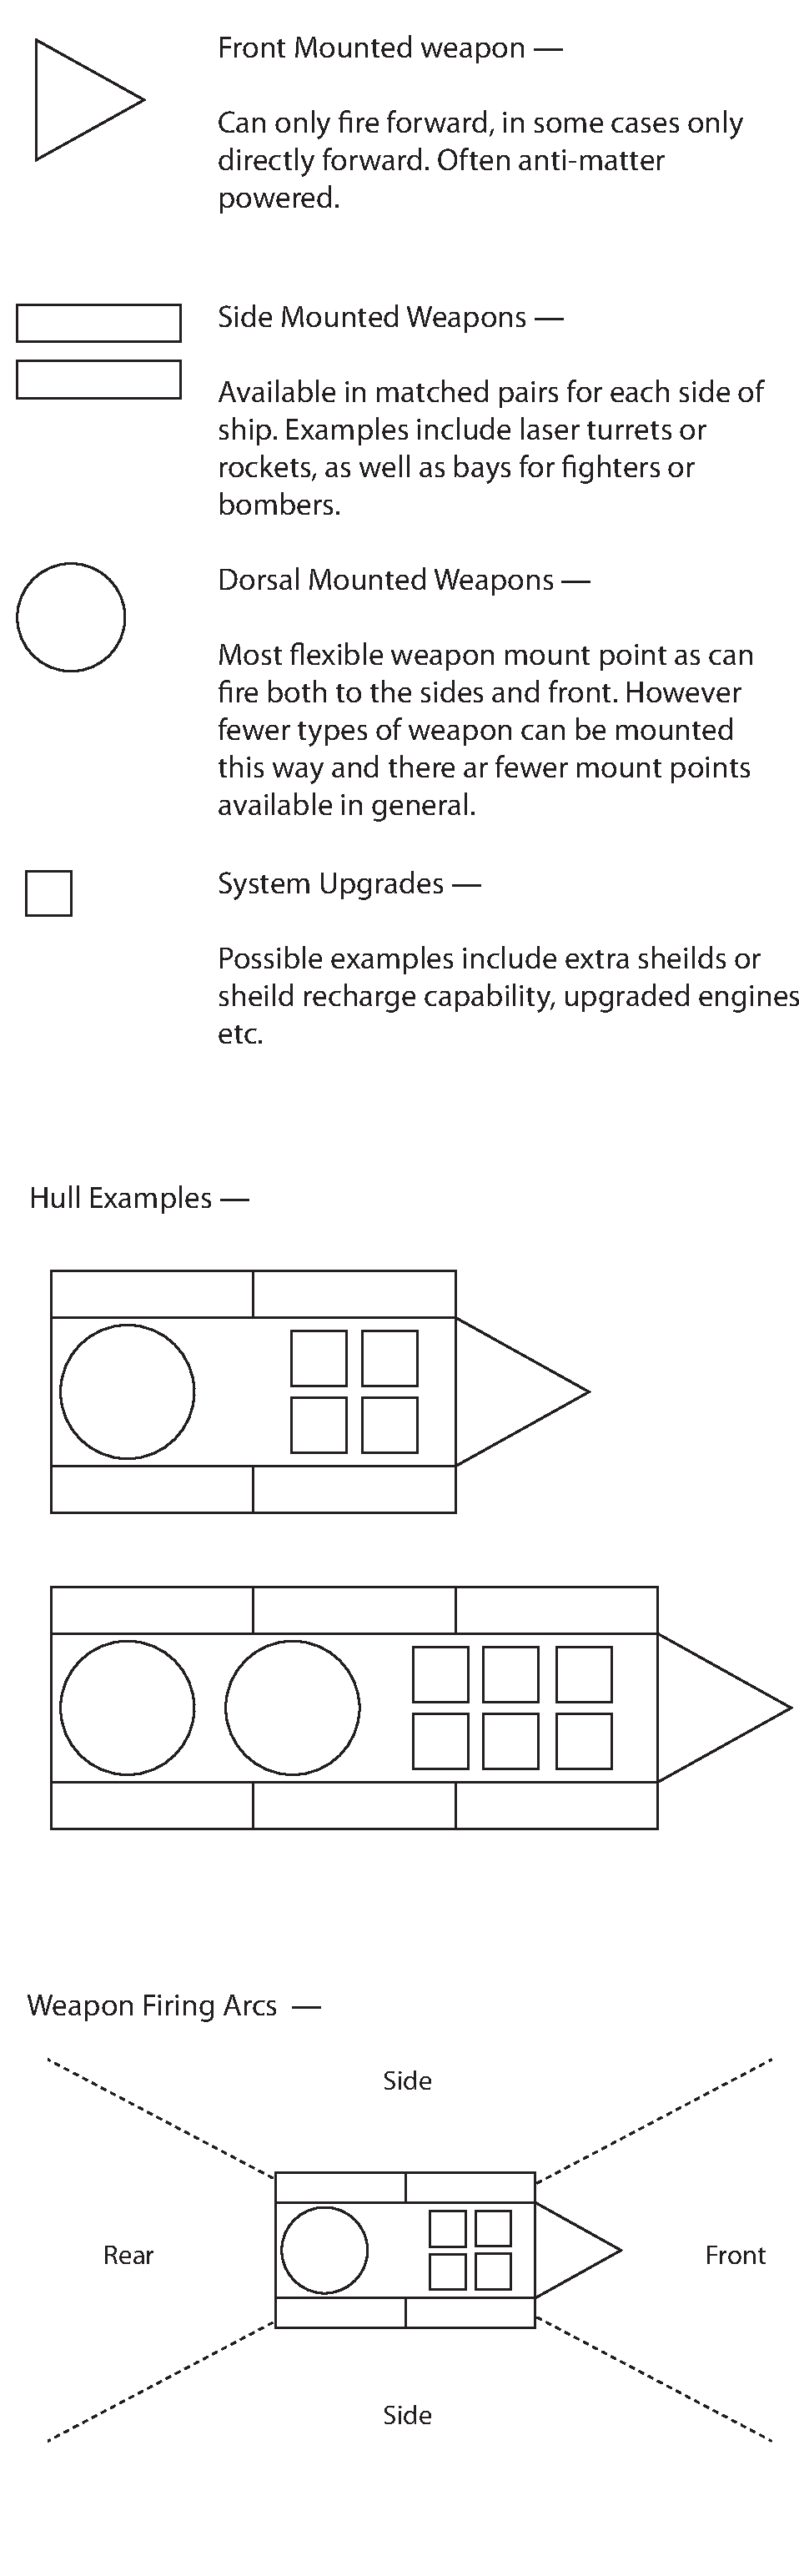
\includegraphics[width=6cm]{res/design/ship_design}
	\caption{Diagrams showing basic conception of ship customisation and weapon configurations. }
	\label{fig:ship_design}
\end{marginfigure}

\begin{description}

	\item[Multiplayer] As a multiplayer game, two players must be able to participate in a battle against each other.
	These players will be on different computers on the same network. This is a more attainable requirement than supporting play over the internet, as latency and packet loss issues will be less intrusive.

	\item[Fleets] Each player will control a fleet of ships. Ships have two health stats: hull and shields. Once hull health has been reduced to zero then the ship is destroyed. However, functioning shields prevent hull damage. It is intended that shields be relatively fast to recharge but hull damage is slow and expensive to repair.

	\item[Ship Customisation] The ships that make up a player's fleet will each have a number of pluggable slots. Prior to a game each player will be able to customise the ships in their fleet by filling these slots with different pieces of equipment. There will be two types of slot: system slots and weapons slots, the latter also split into the areas on the ship it can be installed on. System slots allow for extra internal systems to be added to the ship, for example extra shields or long range scanners. Weapons slots allow the player to choose which types of weapons their ships will use; however, a fleet budget will prevent a user from using the best weapons on every ship. See figure \ref{fig:ship_design}.

	\item[Resource System] Three resources exist within the game: fuel, metal, and anti-matter. These resources are only used by the ships. Fuel maintains a ship's shields, without a shield any damage will be done to the ship's hull. Metal is used to slowly repair a ship's hull after it has been damaged. Anti-matter is a rare resource that is used by the more powerful weapons available.

	Planets generate a constant supply of resources, so players can gain extra resources via planetary capture. The resources generated by the planets owned by a player feed into that player's global stockpile. Individual ships then draw resources from this stockpile.

	% Do ships get resources from the stockpile automatically, or do they have to visit planets?

	\item[Planetary Capture] Planet ownership is the only method of generating resources. Planets can only belong to
	one player at a time at most. To capture a planet, a player must have their ships in control
	of the planet for a certain period of time. If the planet belongs to the enemy then it will
	take twice as long for it to be captured than an unoccupied planet.

	% \item[Tactical Zoom]

\begin{figure*}[t!]
	\includegraphics[width=16cm]{res/design/mockup1}
	\caption[][1em]{Initial mockup of a screen during gameplay, showing a planet, navigation lines, selected ships, minimap, and reports from other ships.}
	\label{fig:mockup1}
\end{figure*}

	\item[Fog of War] Players must not be able to see the state of the entire map unless they control it all. There
	will be three levels to the fog of war: unknown, visited, and visible. Any locations on the map
	that a player's ships have not visited will be `unknown' and the player will not be able to see
	anything that is at that location. Any locations that have been explored at least once will be
	`visited'; the player will be able to see the general layout of the area, but not any details
	such as enemy ships. Finally, any locations covered by planets or ships owned by the player will
	be `visible' and all aspects of the map in the area will be revealed.
	
	\item[AI] A sophisticated artificial intelligence system will be an important component in the game.
	Each player's fleet will be controlled through an AI system. It will use a planning algorithm
	that takes a high level objective given by the player and generates a series of steps to
	achieve that objective. The AI must control the individual ships that make up the fleet; it
	is up to the human player to decide on the overall strategy of the fleet.

	A successful AI system must receive orders and quickly convert them into a sensible plan which it performs and reviews autonomously. If an impossible goal is set, or an existing goal is
	invalidated by changes to the world, then the AI must detect this and act accordingly.

	% Basic AI elements, e.g. pathfinding

	\item[Campaign] A campaign mode will be available which consists of a fixed number of battles between the two players.
	The final battle will be the `showdown' that determines the overall winner. The victor of each of
	the earlier battles will be granted bonuses toward the final battle, giving them an advantage against
	their opponent.

	Between every battle each player will have an opportunity to perform minor customisations on
	the ships in their fleet.

	\item[Operating System Requirements] The game must be playable on recent versions of Mac OS X and Linux. The nature of the libraries that are likely to be used for development make it possible that also supporting Windows will be relatively easy, but this is not guaranteed and no commitment on it is being made at this stage.

% \item[Gameplay]
% mention ship destruction and resources that drained during battle, not loss of ships

\end{description}

\subsection{Non-Functional Requirements}

\begin{description}

	\item[Fun] One of the most important requirements is that the game should be fun to play. Players should enjoy the game and want to play it multiple times.

	\item[Short game sessions] An individual battle should not last too long. If a game is likely to take a number of hours it is a barrier to entry for players as they must schedule large amounts of their time if they are to play at all. The aim should be for an individual battle to last between 20 and 35 minutes. Tournaments or campaigns are possible optional features that could extend this to provide inbuilt support for longer playing sessions.
	
	\item[Approachable]  An end user should be able to play a networked game with minimal configuration (no more configuration required than a typical installation and networking configuration).

	\item[Reliable] Both the client and server should be stable programs that are not prone to crashing. If either were to crash regularly then it would ruin the experience and cause people to stop playing the game.

	The networking component should also be reliable. Minor network disruption should not cause a huge loss in communication between the clients and server.

	\item[Secure] Although the game server will initially be intended for LAN usage it is important that it should not cause a computer running it on the Internet to be exploitable. It should not be vulnerable to attacks such as denial of service, which would stop the machine from performing any other tasks whilst under attack, or remote code execution, which could allow an attacker to take control of the target machine. 
	
	Furthermore, the game system should should not be vulnerable to cheating by modification of the client code, packet injection attacks, or other similar methods of gaining an unfair advantage. 

	% Macromanagement?

\end{description}


\chapter{Results: From Specification to End Product}
\label{ch:game}
\containsfigures{Results: From Specification to End Product}
\containslistings{Results: From Specification to End Product}
\containstables{Results: From Specification to End Product}

\chapterepigraph{Finishing races is important, but racing is more important.}{Dale Earnhardt}

% introduction for this chapter, is not a section



% introduction
% ------------
Our project, irrelevent to implementation language has a very simliar foundation to all games, requiring networking between computers playing the game, graphics engine that can draw the game, assets/sprites for in game entities.

The game's implementation will be designed with an infrastructure that is at the core. All game features will run on top of this infrastructure, having little dependency on other game features, but having complete dependency on the infastrcture. This architecture allows very module design with regards to game features, allowing new game features to be added to the implementation only a slight modification of the infrastructure to include the new feature. By designing the architecture like this, It faciliates a release based schedule.

A high level specification is now available that specifices the elemnts of the game. To bring this high level specification to reality, the game design will be broken down into 3 major releases: Alpha, Beta 1, and Beta 2. Each release specifies the game features that must be in the game. Essentially the game design is broken down into game features, with higher priority game features being specified in earlier releases.
Alpha Release is primarily focused on building the game's Infrastructure, this is the core of the game with all the back end logic that is never seen by the player. By the end of Alpha 1 the game infrastructure is mostly complete, and the game is in a state where game logic can now be added on like modules with little dependency 
Beta 1 and Beta 2 are both game feature oriented, building on top of the existing infrastructure, adding features described in the specification. These releases will heavily focus on meeting the specification's specified game features.

% Laying The Foundation
% ---------------------
Terminology was the first step in the conversion process from specification to working game. 
An initial ambiguity was that many of haskell libraries being looked into had a concept of 'world' which varied dramatically, which in term caused every member of the team to have a different meaning for the word. This caused many misunderstandings until an internal terminaology was devised within the team to describe common terms such as 'client state'. Once the terminology hurdle was solved, The team was able to share design ideas efficiently.

By the end of alpha Stage a working 'game' was needed, somethat that could be used as a base to start adding game features.

The infrastructure must provide a platform that the game features can be implemented ontop of, Hence it must contain:
\begin{itemize}
\item Server-Client communication
\item Rendering capabilities for assets
\item Game loop
\item Model of game components
\end{itemize}

Mistakes at this stage will cost heavily later down the line, because so much will dependend on the infrastructure. 

\begin{comment}

alpha stage layout
------------------
features wanted at this stage:
    - networking
    - server client loop
    - game update model (lock-step no no no)
    - ship move orders
    - world rendering(easy debugging)
    - more focus around infrastructure than features
    
    
  - lack of libraries, implemeintg our own networking, GUI library.
  - implementation of network library.
  - server and client not distinquished just yet
  - game loop
  - lock-step big part
    - arguments for and against
  - integration of assets into game
  - API for game how entities are added
  - how generating diffs will work

  - infrastructure components
    - networking
    - gameploop
    - how the server and client synchronize
    - graphics


\end{comment}


% sections
\clearpage
\section{Server-Client Synchronisation}

\newcommand{\stepOneName}{lockstep}
\newcommand{\stepTwoName}{simple server client}
\newcommand{\stepThreeName}{server client with simulation}

% topology of network(star diagram, what server does, what client does)
\begin{marginfigure}
	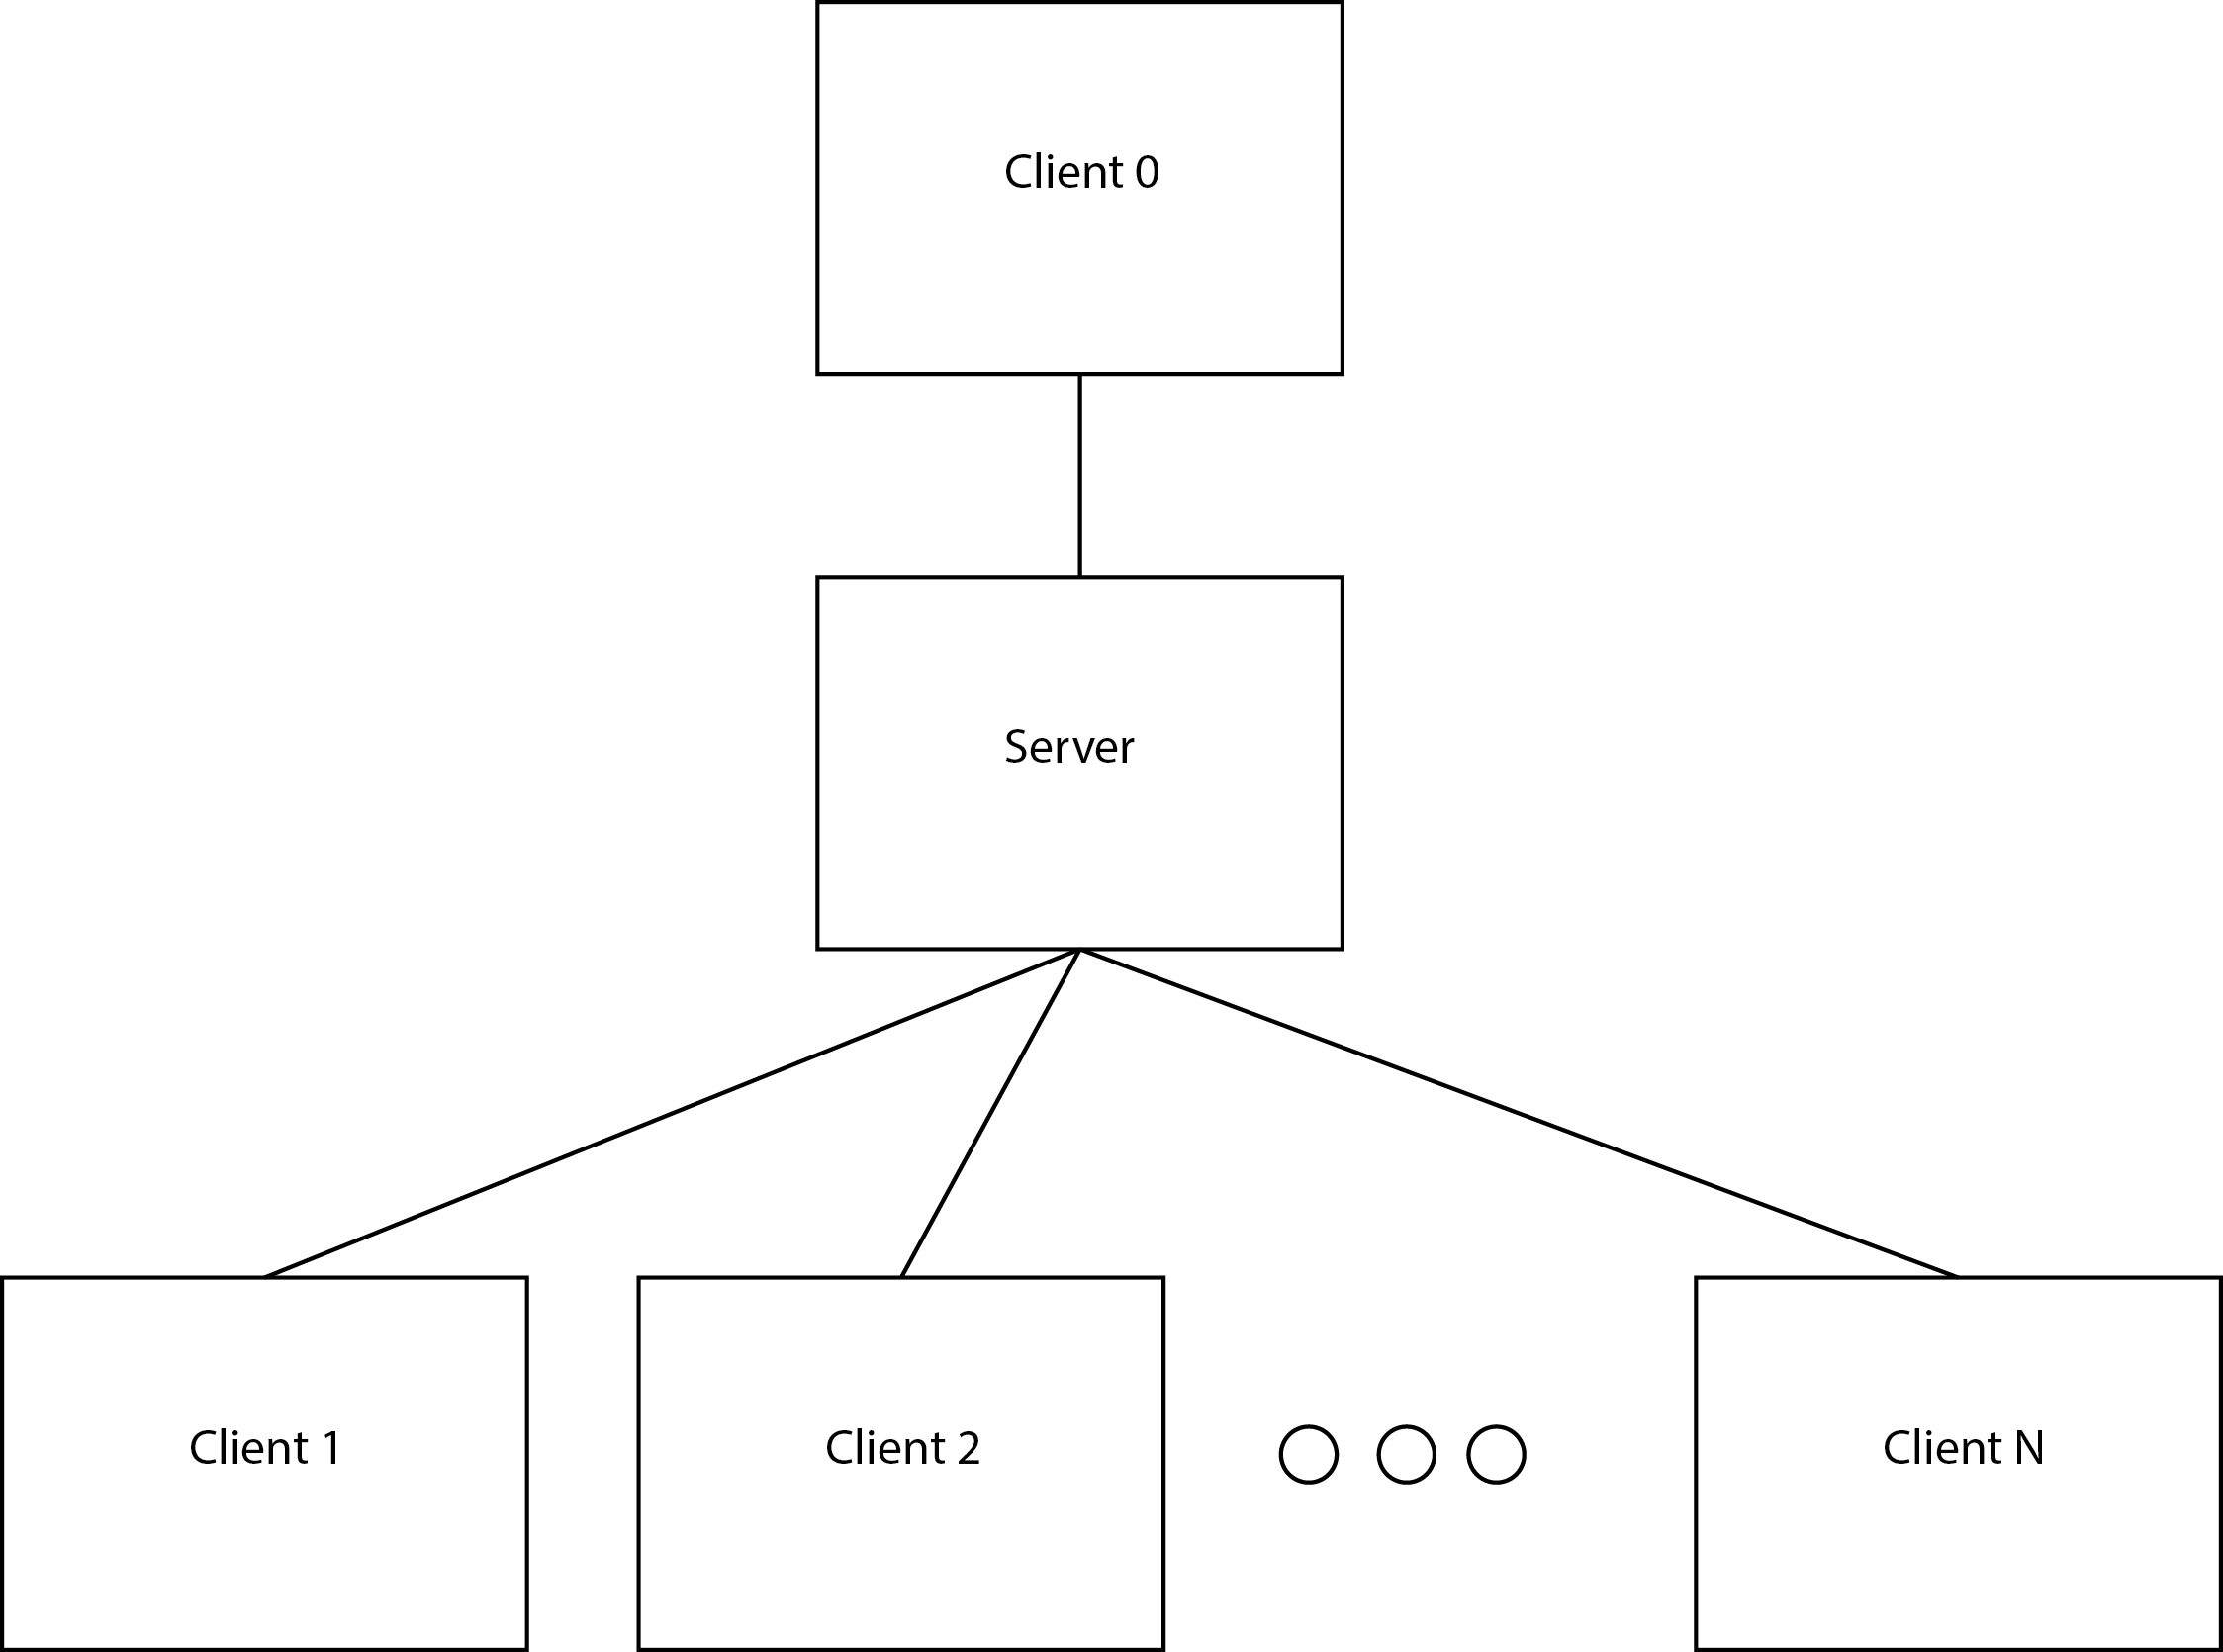
\includegraphics{res/computer_communication_architecture/NetworkTopology.png}
	\caption{
	network topology for multiplayer.
	}
	\label{fig:serverClientSychNetworkTopology}
\end{marginfigure}

The topology is a typical Star Network, with server in centre, and all clients only connecting to server.
There are $N+1$ player connected, where client 0 is the client that is hosting the server.
Since client 0 is hosting the server, they have special permissions to stop the server at any point, ending the game.
This topology greatly simplifies the requirements of the networking, because every client has to only connect to server, and receive all its updates from 1 single place. 

% protocol for synching game states between client server (command, update)
Figure \ref{fig:loops} gives a good representation how the server and a given client communicate.
Both the server and client have a full copy of the model representing the game state.
Their were a variety of benefits from this, the least of which it allowed the clients to scroll around the map without requiring any network traffic.

When the player gives an order, i.e. to move a ship to a given destination, that order is sent to the server in the form of a command.
On the server side, that command is used to 'update' the server's game model. Now the server's game state is at a later version than the clients. The server generates updates that can be applied to all client's game states to bring them to the same version as the server's version.

An example of an update message is: A ship has been given a move order to a location on opposite side of map.
Since their is no simulation on the client side, the ship will only move if the server sends an position update to the clients, moving it slightly closer to its destination. This means that for every time step, every ship that is moving will require an update message send across the network to every client. 

The move update will look something like this:

\begin{margintable}
    \begin{tabular}{l l l l l}
    \toprule
    \emph{shipID} & \emph{x} & \emph{y} & \emph{direction x} & \emph{direction y} \\ 
    \midrule
    43 & 10 & 15 & 0 & 1 \\
    \bottomrule
    \end{tabular}
    	\vspace{1em}
	\caption{example of a position update message}
	\label{tab:positionUpdateExample}
\end{margintable}

Instead of the server telling the client where the ship's destination is, and letting the client move the ship their, the server tells the client when to the next jump location. In the example in Figure \ref{tab:positionUpdateExample} the ship with ID 43 has been given a position update to the new coordinates (10,15), facing North which is (0, 1).

Their are a variety of updates message, depending on which part of the game needs to be updated. 
Originally there was only 3 types of updates:
\begin{description}
\item[addEntity] used for adding an entity to the game. It contains the entity being added to the game.
\item[deleteEntity] used for deleting an entity. An example of use would be when an entity was just blown up. Only contains the entiyID
\item[updateEntity] most common update, used to update an entity. It contains the new entity, and the existing entity is replaced with the entity inside this update.
\end{description}

Having 3 updates provided a very simple design. 
2 out of the 3 updates(addEntity and updateEntity) contains an entity object which is very large in size.
To send an entity object across the network can be very slow and should only be done when necessary.

The addEntity update needs to contain an entity because that entity is currently not in the game, so all the fields of the entity need to be sent across to all the clients. Since addEntity is primarily used at the start of a game when all the entities are loaded into the game, this is not a problem.

However the updateEntity update is sent every time an entity changes location, direction, targets, etc.
Each time an entity's field changes the entire entity must be sent across the network to all the clients.
Not only is this taking up a large amount of bandwidth, but it is sending a large proportion of redundant fields which haven't been changed.
The solution to this was to split the updateEntity update into multiple updates, each one for a common update usage.
The different types of updates to an entity were identifies and a new update message was given to it. 
Table \ref{tab:updateMessageTypes} contains the update messages devised.

\begin{table}
    \begin{tabular}{p{5em} p{15em} p{6em}}
    \toprule
    \emph{Update Type} & \emph{Description} & \emph{Fields} \\
    \midrule
    position & used when both the ship's location and direction has changed & entityID, location, direction \\
    order & when a ship's orders change & entityID, order \\
    goal & when a ship's goal changes & entityID, goal \\
    plan & when a ship's plan to achieve its goal changes & entityID, plan \\
    health & when a ship's hull or shields health changes & entityID, hull health, shield health \\ 
    \bottomrule
    \end{tabular}
    	\vspace{1em}
	\caption{each type of update message, description of its usage, and the fields it will contain}
	\label{tab:updateMessageTypes}
\end{table}

Now, when a ship's field, say direction changes, the direction update message is used instead of the old entity update message.
This is significantly cheaper with regards to network usage because only the ship's ID and new location are sent.

% network traffic calculation
Their were concerns that the volume of traffic required to maintain all the client's game states updates would still be too great for a playable game.
Therefore a traffic analysis was done to estimate how much network traffic would actually be required.
When assumptions are made concerning the game, such as number of ships, number of game steps per second, etc, worst case scenario will be assumed giving the limitations of the game, IE we will know the maximum number of ships the game can have before the game becomes effects by network bandwidth.



The size of each update message will need to be estimated as well as how frequently that message will be sent.

First, the size of field types will need estimating using language independent types such as int, float, double, etc.
This is done in Table \ref{{tab:positionUpdateExample}
\begin{margintable}
    \begin{tabular}{p{5em} p{5em}}
    \toprule
    \emph{Field Type} & \emph{Field Size/bytes} \\
    \midrule
    int & 4 \\ 
    long & 8 \\ 
    float & 4 \\
    double & 8 \\    
    \bottomrule
    \end{tabular}
    	\vspace{1em}
	\caption{example of a position update message}
	\label{tab:positionUpdateExample}
\end{margintable}

Now we have estimates of size for the different types, we can assign types to the fields of the message

\begin{margintable}
    \begin{tabular}{p{5em} p{5em} p{5em}}
    \toprule
    \emph{Field Name} & \emph{Size/bytes} \\
    \midrule
    entityID & 4 \\ 
    location & 8 \\
    direction & 8 \\ 
    order & 15 \\
    goal & 9 \\ 
    plan & 100 \\ 
    hull & 4  \\ 
    shield & 4  \\  
    \bottomrule
    \end{tabular}
    	\vspace{1em}
	\caption{example of a position update message}
	\label{tab:positionUpdateExample}
\end{margintable}



For the plan field, it was assumed that each action within the plan was approximately 20 bytes, and that the average plan has 5 steps.

The following table estimates the size of a message to sent across network:
\begin{center}
    \begin{tabular}{| l | l | l |}
    \hline
    Update Type & size / bytes & frequency per game step \\ \hline
    position & 20 & 1 \\ \hline
    order & 19 & 0.2 \\ \hline
    goal & 14 & 0.3 \\ \hline
    plan & 104 & 0.3 \\ \hline
    health & 12 & 0.1 \\ 
    \hline
    \end{tabular}
\end{center}


Now we have the size and frequency of each update message, we can calculate how many bytes are sent to a single client every game step. 
$$ bytes = 20*1 + 19*0.2 + 14*0.3 + 104*0.3 + 12*0.1 $$
$$ bytes = 60.4 $$

We have $S$ representing the number of game steps per second, and $N$ representing the number of clients connected to server.
The number of bytes the server sends per second is
$$ bytes = S * N * 60.4 $$

We now have a formula to calculate network traffic, we need to apply to to various values of $N$ and $S$.

% s=15, 30, 45, 60, n =2, 4, 8, 16
\begin{center}
    \begin{tabular}{| l | l | l |}
    \hline
    S & N & kB/second \\ \hline
    15 & 2 & 1.77 \\ \hline
    \hline
    \end{tabular}
\end{center}

-------------------------- worked upto here ------------------


constants for calculation:
\begin{center}
    \begin{tabular}{| l | l |}
    \hline
    Constant & Value \\ \hline
    world updates / second & 30 \\ \hline
    ships & 40 \\
    \hline
    \end{tabular}
\end{center}

A 

The next step was to calculate the size of a ship update message.

Hence a single ship movement update message would be:
$$ size = (shipID, x, y, directionX, directionY, hullHealth) = 5 * 4 bytes = 20 bytes $$
To send a single ship update to a single client is 20 bytes.



			world updates per second 30
			ships in world = 40
			bullets in world = 1000
			ship movement update = (shipId, x, y, direction) = 4 * 4bytes = 16 bytes.
			bullet movement update = (bulletId, x, y, direction) = 4 * 4bytes = 16bytes
			per client:
				per update:
 					ship data = 40 * 16bytes = 640bytes
					bullet data = 1000 * 16bytes = 16000bytes
					total data = 16640bytes
			    per second = 30 * 16640 = 499200bytes = 487.5KB/S
			3 clients = 3 * 487.5KB/s = 1462.5KB/s = 1.43MB/s

% advantages/disadvantages of lockstep
% advantages/disadvantages of server client with simulation


\begin{comment}

This section talks about how multiplayer was achieved.
This includes the network topology.
server-client allows master copy to exist on server.

- master copy of world on server
- clients perform no logic, only apply updates to
- 




----------------------------------- old gay -----------------------------------------

we need to work out how the computers talked to each other very early on
2 considerations: peer 2 peer, client-server
  - advantages of peer 2 peer
  - advantages of peer server-client
  - why server-client chosen 
  - issues experienced with server-client
    - jumpy ship movements
\end{comment}

The game was designed around being multiplayer, so our first goal was to decide how the player's computers would talk to each other.
Since their was an arbitrary number of players (greater than 1), We needed a system that would scale, but would also be robust.
The game was expecting all players to be on the same LAN (Local Area Network), hence a high bandwidth was available for the communications.

There are 3 strategies for the interactions between computers:
\begin{itemize}
\item \stepOneName
\item \stepTwoName
\item \stepThreeName
\end{itemize}


\begin{marginfigure}
	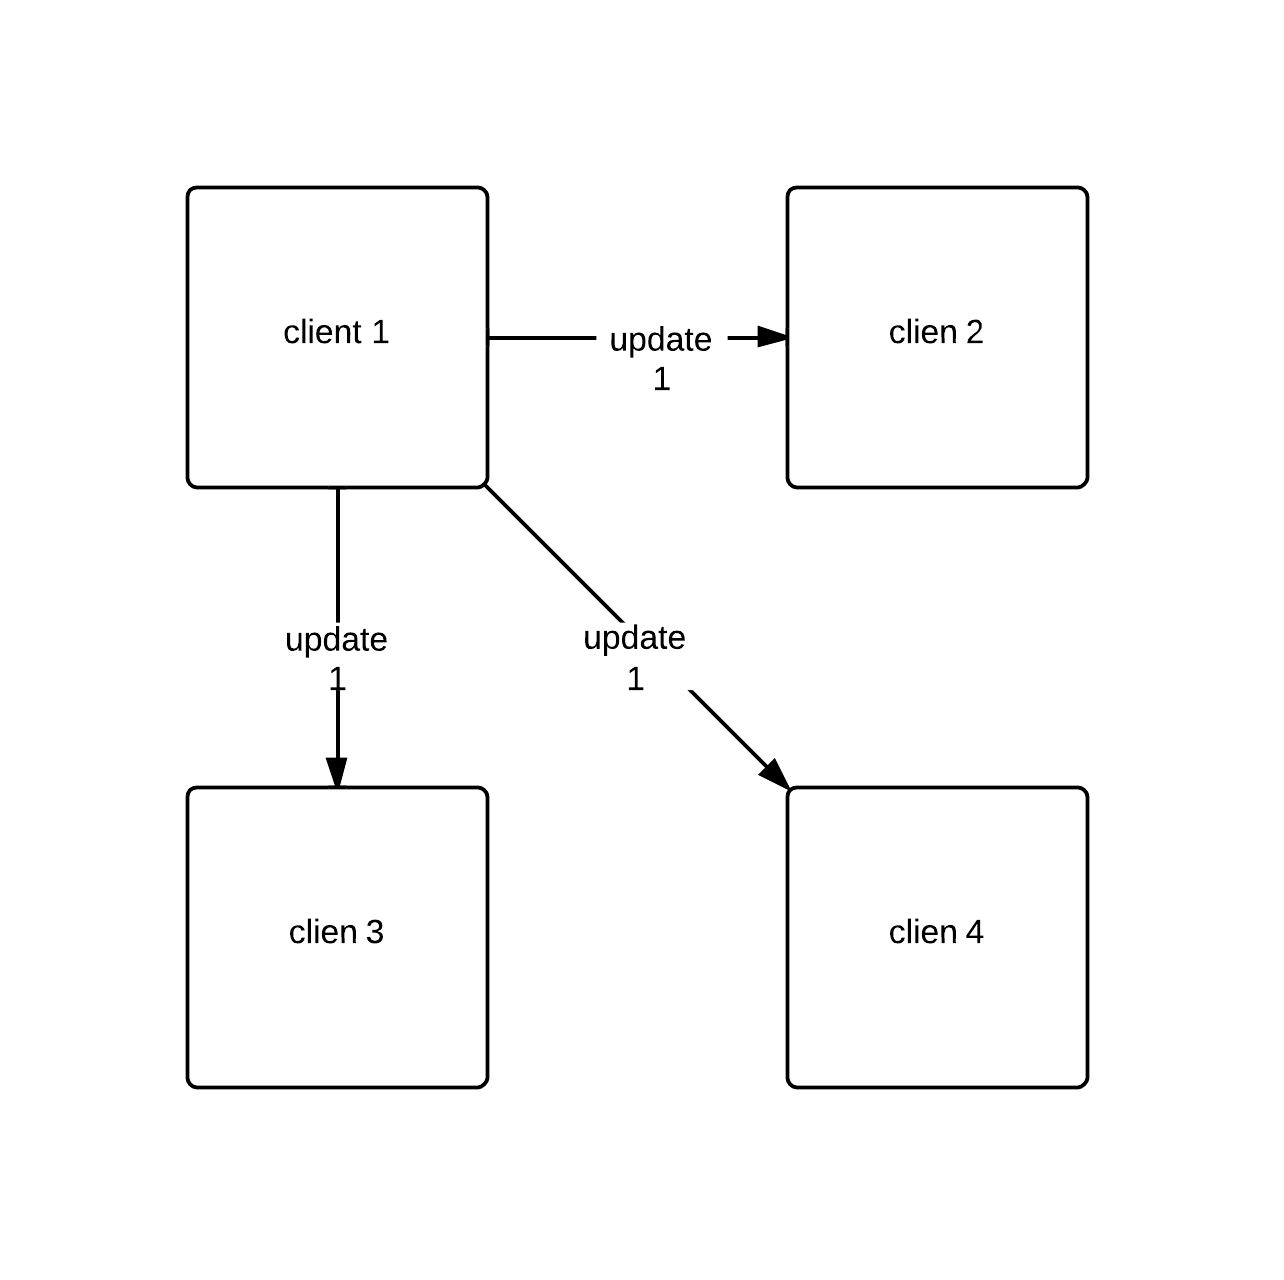
\includegraphics{res/computer_communication_architecture/ServerClientSynchronizationP2P.png}
	\caption{
	\stepOneName : 4 clients connected. client 1 has just modified its game state, so it send the update to all other clients.
	}
	\label{fig:serverClientSychP2P}
\end{marginfigure}

% what
\stepOneName is a peer to peer strategy, in which each computer has a full model of the game. Figure \ref{fig:serverClientSychP2P} shows an example of this strategy. 
Their are 4 computers within game. Each client (client 1, client 2, client 3, and client4) have a full copy of the game.
When client 1 updates performs some actions, they must update their game state, and send this update to all other clients.

\begin{marginfigure}[-30em]
	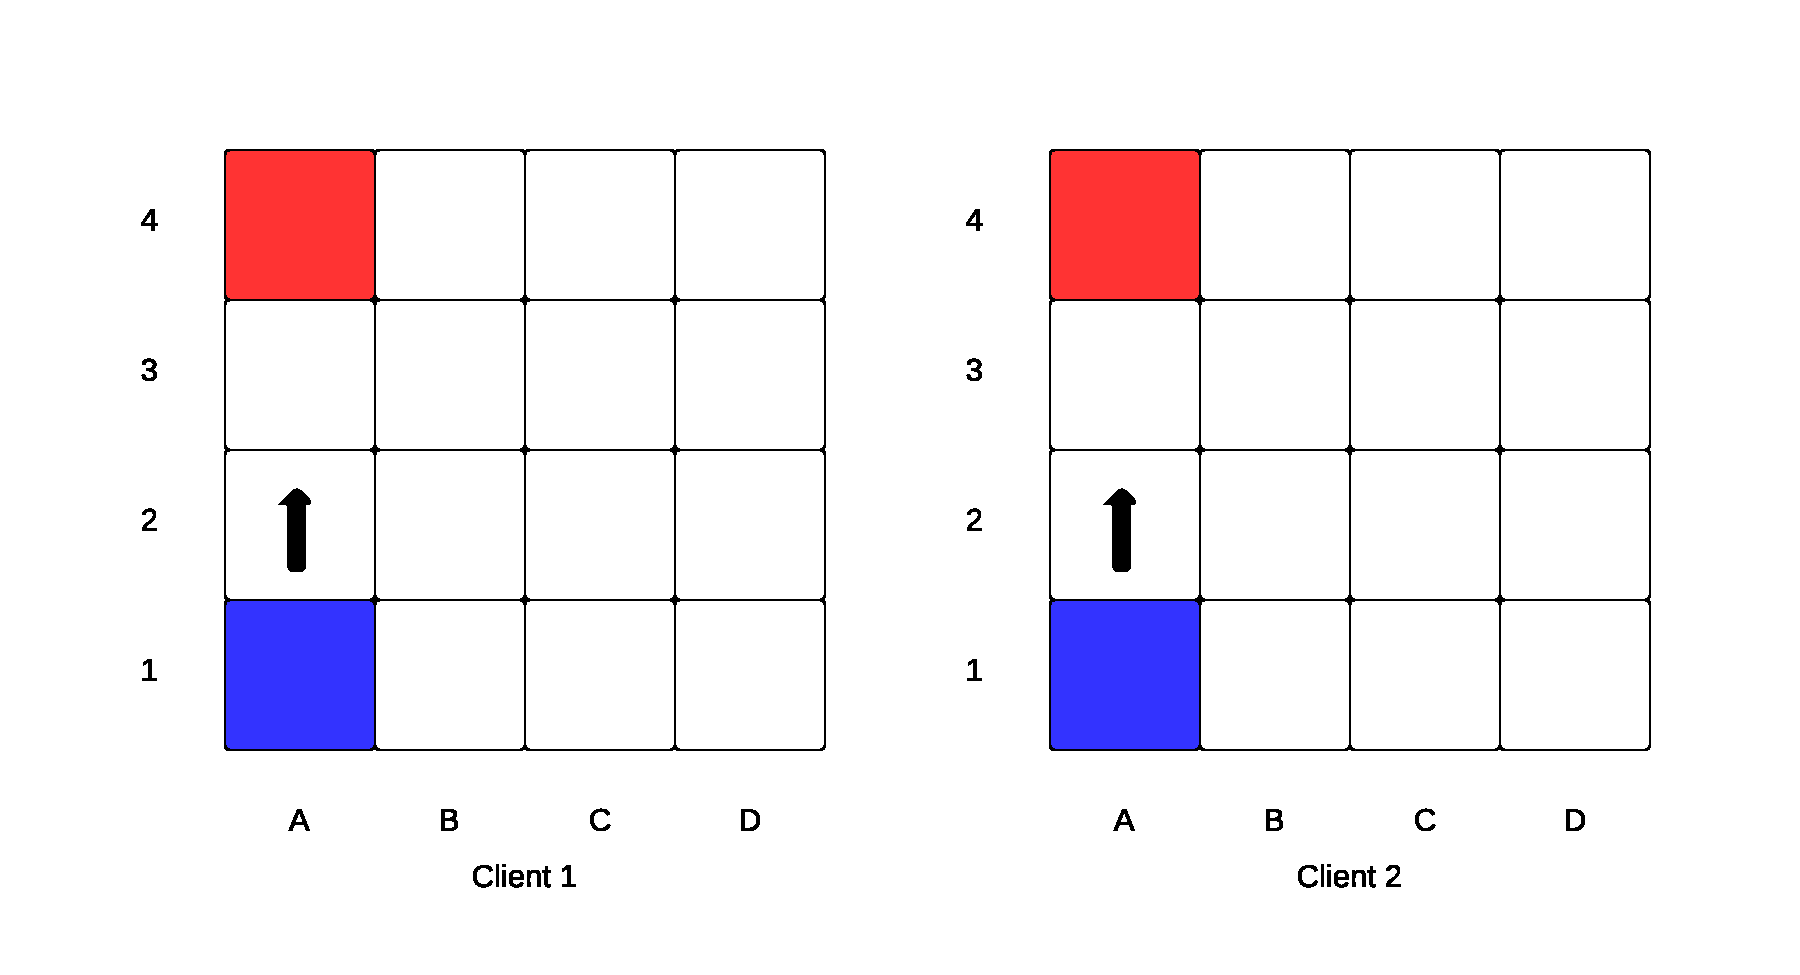
\includegraphics{res/computer_communication_architecture/ServerClientDesynchronisation1.pdf}
	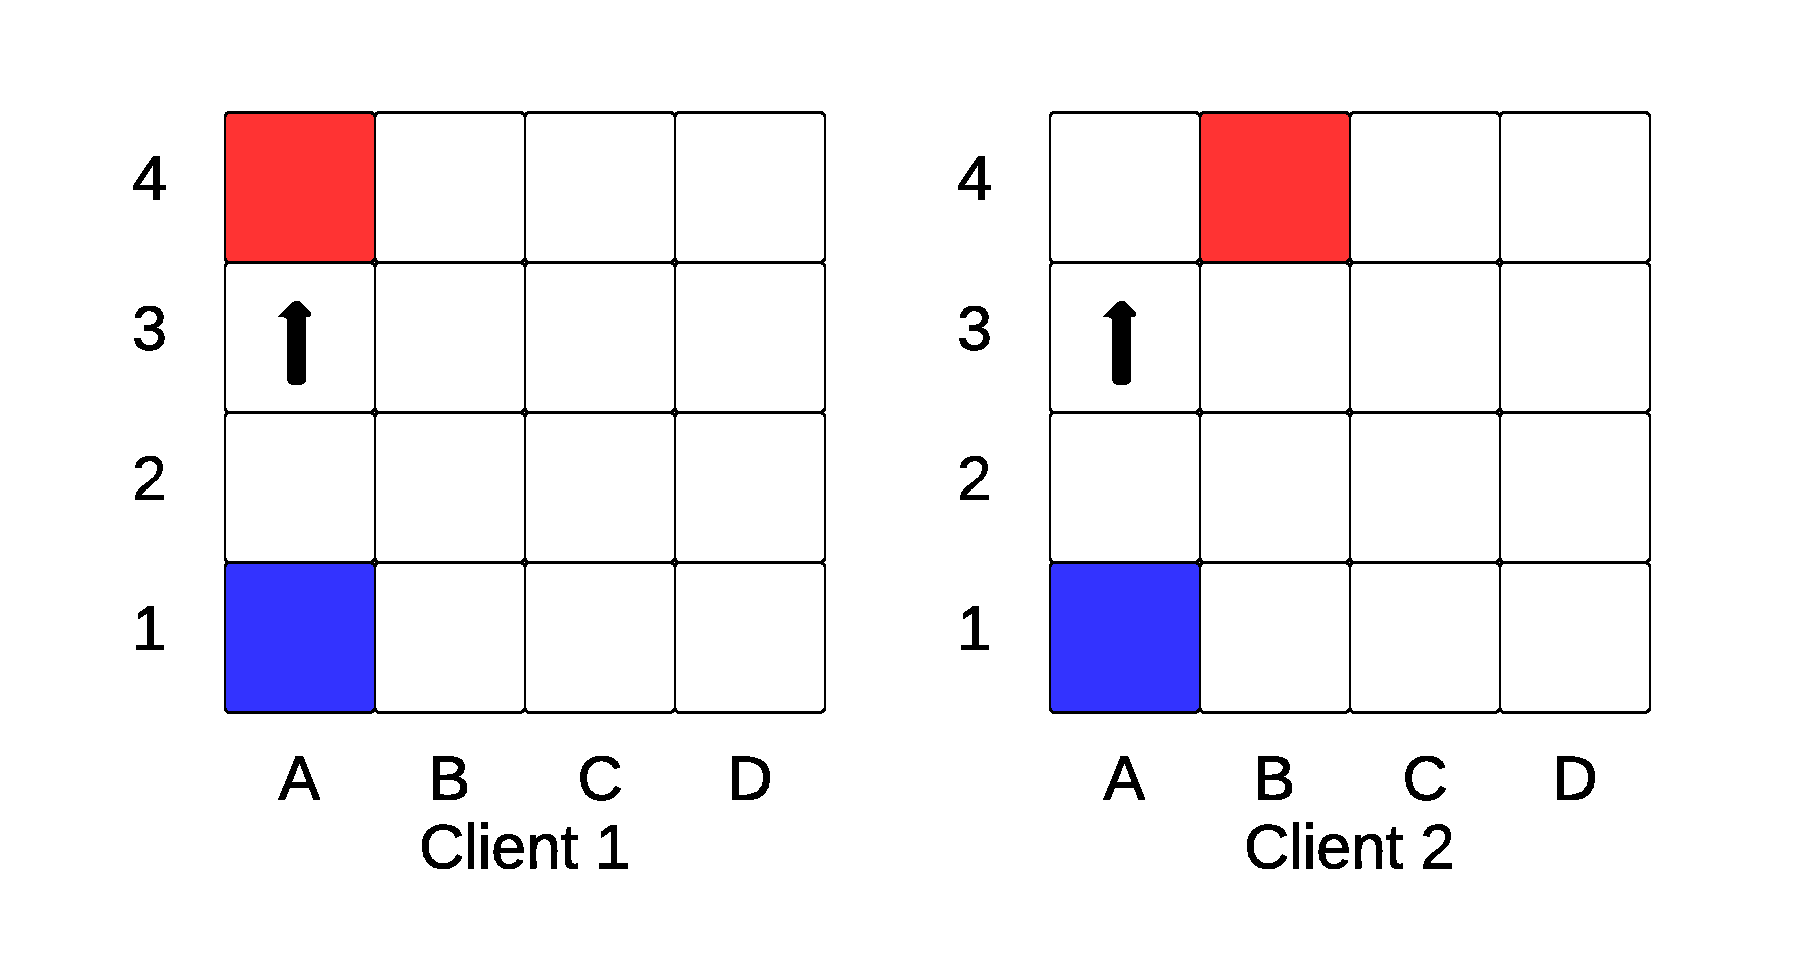
\includegraphics{res/computer_communication_architecture/ServerClientDesynchronisation2.pdf}
	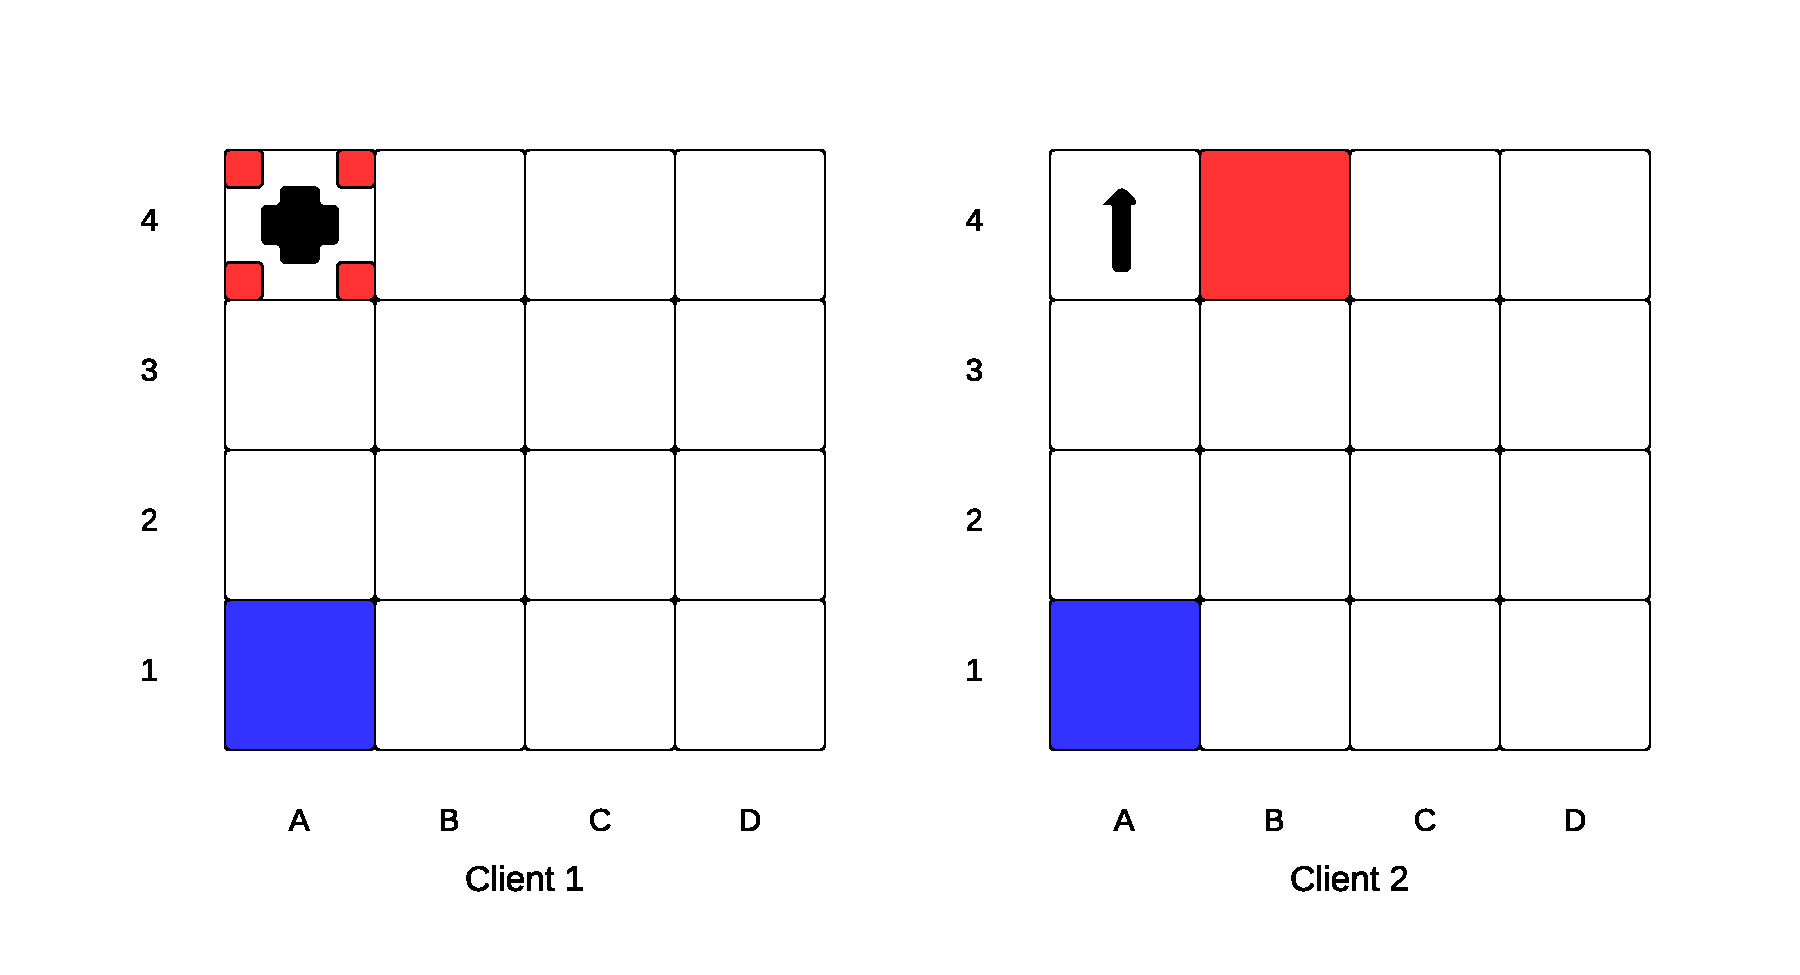
\includegraphics{res/computer_communication_architecture/ServerClientDesynchronisation3.pdf}		
	\caption{
	\stepOneName : example of desynchronization when using the \stepOneName strategy. Client 1 on left, client 2 on right. 
	Each diagram represents state of game for that clients at a given time period.	3 diagrams vertically aligned, First one is top, second one is middle, third one is bottom.
	}
	\label{fig:serverClientDesync}
\end{marginfigure}

% advantages
%   playable with slow networks
This strategy means players can continue to play games on networks with high latency, without any lag. When packets are delayed, the client can continue to play the game, and the game is updated when the packet arrives.
%   no dedicated server required
No client is picked to act as server, which causes game to end if that selected client disconnects.
Since all clients act as server, any client can disconnect and the game continues, providing more robustness which is highly desirable for games with long game intervals, such as Civilization series\cite{civilizationInMyPants}.



% disadvantages
%   disynchronization
Maintaining synchronisation when using a peer-2-peer protocol can be very challenging from a technical point of view, with non-determinism being caused by messages being received by clients at different times causing race conditions.
When this happens in a game, it can cause clients game states to desynchronise.
For example, In Figure \ref{fig:serverClientDesync}, there are 2 clients.
%   corrupted client can effect the entire game



% res/computer_communication_architecture




% lockstep
%   - each client has the master copy of the world
%   - when a client does something, it tells all others
%   - problems:
%     - desycnhronization
%     - currupted client fucks up everyone

% simple server client
%   - it's what we've implemented
%   - no simulation on clients
%   - 1 server that has master copy
%   - server does all processing and sends updates to clients
%   - clients just render the world and send commands to server

% server client with simulation
%   - similar to simple server client but client does 'some' simulation. They in no way can effect the world.
%   - for instance if client knows ships destination and current location it can render the ship graciously moving instead of jumping on every update.


\clearpage\section{Modelling the Game}
\label{sec:model}

% what this section talks about
%   - graph of objects and relations
%   - what each model object represents and is
%   - difficulties developing the model
%   - model: sector, game, entity, ship, plan, goal, ship action, ship class, ship configuration, weapon, system, weapon slot, system slot, fleet, Formation, client state
% what is a game model
% early on
% 

The model that makes up the game consists of the internal representation of the various game entities, such as ships and planets, as well as the business logic that is used to manage and control them and the relationships between them. During the alpha phase, this model was rather simple as it only existed to store the locations of the entities. As development progressed, it grew in complexity and feature completeness. Currently there are two sets of models: one for the fleets of ships, and the other for the map of planets and spacelanes.\sidenote{Spacelanes are connections between some planets that allow ships travelling along or nearby them to move more quickly. See Section~\ref{sec:pathfinding} for details.} This section will describe and discuss these models and the reasonings behind their design.

\subsection{Sectors and Planets}

\begin{margintable}
    \begin{tabular}{p{4em} p{11em}}
    \toprule
    \emph{Field} & \emph{Description} \\
    \midrule

    Name & Sector name \\
    Size & Sector dimensions \\
    Spawn points & List of locations where different players' fleets are spawned \\
    Planets & List of planets in the sector \\
    Spacelanes & List of spacelanes that connect the planets \\

    \bottomrule
    \end{tabular}
    \vspace{1em}
    \caption[Fields of the Sector model]{Fields of the Sector model.}
    \label{tab:sector-fields}
\end{margintable}

The different game maps are known as sectors. A sector models all of the planets in a battle, how they are connected with spacelanes, and where the different spawn points are located.\sidenote{Spawn points are locations where a player's fleets will be created} The actual fields that make up the sector model are shown in Table~\ref{tab:sector-fields}. Sectors have different sizes because it allows the players to customise the play time required for a battle to some degree. Choosing a larger sector will typically result in a longer battle than smaller ones. The specification has a requirement for short battles, but it is good to add some flexibility to allow players the freedom to decide how to enjoy the game. It could have been possible to have static spawn points that are enforced for all sectors, for example spawning players in the corners of the sector so that they are as far apart as possible. However, the actual design has per sector spawn points so that the spawn points can be customised to be as fair as possible relative to the layout of the planets within the sector. This decision was made to make the game as balanced as possible to maximise the enjoyment of all players.

% The sector specifies which planets are includes as well as which planets are connected by space lanes as shown in Figure \ref{fig:model:sectorRelation}

% \begin{marginfigure}
% 	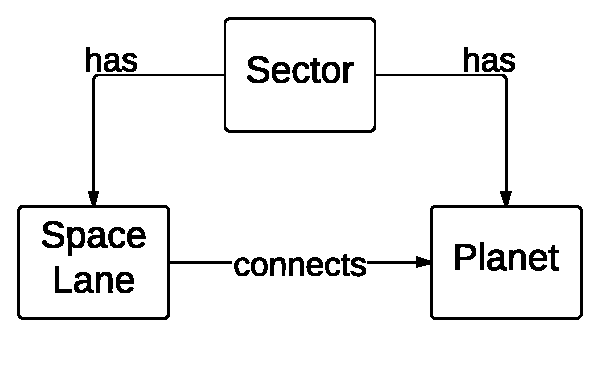
\includegraphics{res/model/sector.pdf}
% 	\caption{relationship between setor, planet, and space lanes}
% 	\label{fig:model:sectorRelation}
% \end{marginfigure}

\begin{margintable}
    \begin{tabular}{p{4em} p{11em}}
    \toprule
    \emph{Field} & \emph{Description} \\
    \midrule
    Name & Planet name \\
    Ecotype & Type of planet, e.g. primordial, ocean, or desert \\
    Location & Location of planet within the sector \\
    Resources & Quantity of resources generated by the planet if captured \\
    Capture status & Current owner of the planet, if any, and by how much they have captured it \\
    \bottomrule
    \end{tabular}
    \vspace{1em}
    \caption[Fields of the Planet model]{Fields of the Planet model.}
    \label{tab:planet-fields}
\end{margintable}

The list of planets that make up the sector are specified using the planetary model. Planets are modelled in such a way as to have a number of different fields that make the planet unique. Table~\ref{tab:planet-fields} gives a breakdown of the properties that comprise the model of a planet. Just like sectors, planets have a name to allow players to easily reference a specific planet instead of having to use location information or a numerical identifier. One of the most interesting pieces of the planetary model is the \emph{ecotype}. The ecotype of a planet specifies the type of ecological system that the planet represents, for example the ocean ecotype is used for planets that are almost entirely covered by water. This ecotype has a big effect on the planet because it determines the quantities of the different resources found in the planet.\sidenote{The use of resources is detailed in Section~\ref{sec:resources}} For example, some ecotypes will have a greater proportion of metal (e.g.\ the metal ecotype). However, the quantity of resources stored by a planet is actually represented by a separate field instead of being statically determined by the ecotype. This was done to make it possible to add some more variety to the different planets. For example, it could be possible to use a random number generator to set the quantities of resources in a planet within the range specified by its ecotype. Currently all resource quantities are specified statically, but this potential enhancement would add some variation to the battles to keep the game interesting for regular players.

% TODO fix margin diagrams, all appearing below the page (invisible)
% \begin{marginfigure}
% 	
\includegraphics{res/planets/star.png}
% 	\caption{ecotype: star}
% 	\label{fig:model:starPlanet}
% \end{marginfigure}
% 
% \begin{marginfigure}
% 	
\includegraphics{res/planets/OceanPlanet.png}
% 	\caption{ecotype: ocean}
% 	\label{fig:model:oceanPlanet}
% \end{marginfigure}
% 
% \begin{marginfigure}
% 	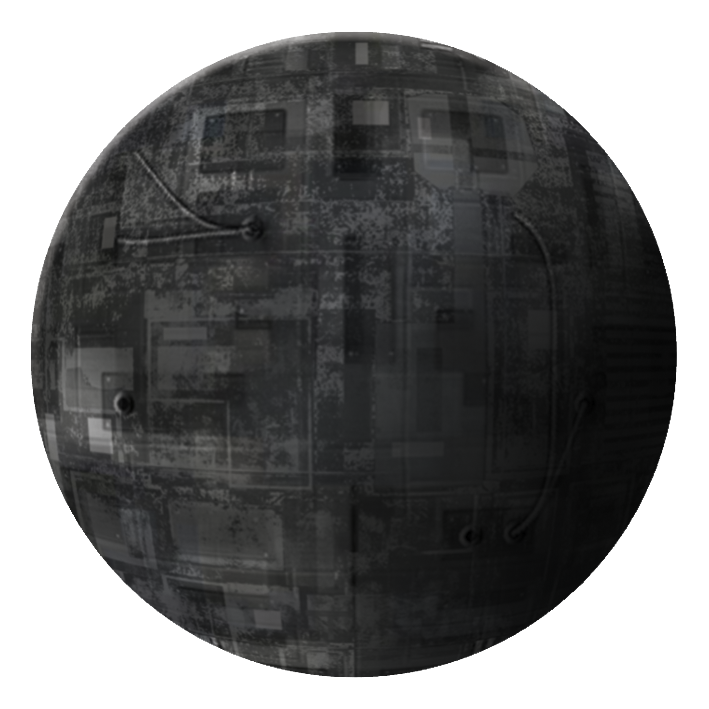
\includegraphics{res/planets/metal-planet.png}
% 	\caption{ecotype: metal}
% 	\label{fig:model:metalPlanet}
% \end{marginfigure}

\subsection{Ships, Classes and Configurations}

\begin{margintable}
    \begin{tabular}{p{4em} p{11em}}
    \toprule
    \emph{Field} & \emph{Description} \\
    \midrule
    Location & Current location of the ship within the sector \\
    Direction & The direction the ship is facing \\
    Damage & How much damage the ship has taken \\
    Order & Current order for the ship \\
    Goal & Current goal the ship is trying to achieve \\
    Plan & Current plan to execute in pursuit of the goal \\
    Targets & List of enemy ships that the ship is attacking \\
    Config. & Class of ship and its customisations \\
    \bottomrule
    \end{tabular}
    \vspace{1em}
    \caption[Fields of the Ship model]{Fields of the Ship model.}
    \label{tab:ship-fields}
\end{margintable}

The second set of models deal with the fleets of ships that are controlled by each player. A fleet is simply a list of ships which a client sends to the server having chosen which ships to include and having made their customisations to these ships. The representation of a ship is actually broken down into a generic ship model and its specific configuration. The general ship model contains the configuration as well as the attributes that are updated during game play, such as the ship's orders and plans, and its current location and direction. The full list of fields for this model is shown in Table~\ref{tab:ship-fields}. The use of location, direction, and damage should hopefully be obvious. They can be updated every tick by the server's main loop as the ship moves around the sector and engages with the enemy. Orders, goals, and plans are used by the artificial intelligence that controls the ships, see Section~\ref{sec:ai} for more details. The list of targets that a ship is currently attacking is also controlled by the artificial intelligence. The most interesting part of the ship is its configuration which specifies what ship class it is and the customisations that have been applied by the user.

The ship configuration contains the chosen ship class along with the lists of weapons and support systems that the player selected to add to the ship. The ship class represents the type, or blueprint, of ship specifying the basic statistics of the ship. The set of statistics defined by the class is: speed, hull health, shield health, details of each of the weapon slots, details of the support system slots, and the cost of the ship. These statistics are used by the simulation code in the server to determine how the ship moves, how much more damage it can sustain before being destroyed, how much damage it does to the enemy ships it is attacking, and so on. A player is able to select the set of ship classes that they wish to include in their fleet, but they are restricted by a fixed budget. There are three ship classes that come with the game by default: corvette, destroyer, and dreadnought. The corvette is the smallest and quickest ship that can only be given one weapon. The destroyer is of middling strength and speed, it allows for five weapons to be added. Finally, the dreadnought is the largest and slowest of the three, but it packs the largest punch by supporting up to nine weapons.

This layered model approach to representing the ships was used to separate the different types of data that have to be stored. The ship model deals with the dynamic data that is updated during gameplay, the ship class is concerned with the static statistics that define the ships behaviour, and the configuration stores the user's customisations. This is useful because it allows a more efficient method of storing custom fleets on disk. Only the list of ship configurations needs to be kept since the class data is the same for all ships of the same type so can be loaded at run time and the rest of the ship data is only relevant during a battle.

% \begin{marginfigure}
% 	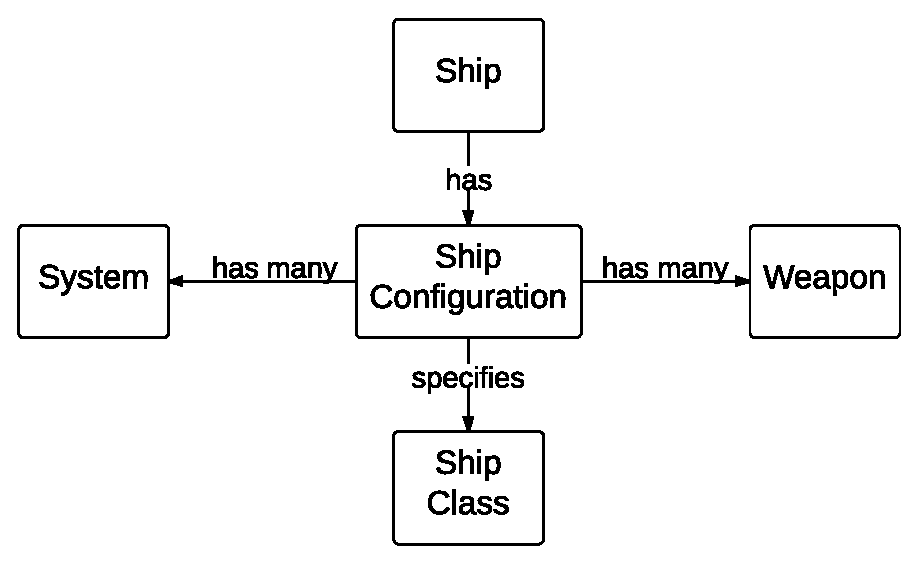
\includegraphics{res/model/ship.pdf}
% 	\caption{ship layout}
% 	\label{fig:model:shipRelation}
% \end{marginfigure}

\subsection{Weapons and Support Systems}

% TODO all
% talk about the ships firing arc
% ship weapons(different types of weapons, differences, firing arcs, ranges), do we have more than lasers to talk about?, target targeting)

Before a battle is started, a user is able to customise the ships that make up their fleet. They do this by first selecting the types of ships to use and then filling the pluggable slots with extra parts. There are two types of part: weapons and support systems. Weapon slots are arranged in three different locations around the ship. Side weapons are used to fire to the port and starboard of the ship. The front weapon slot, if present on a ship, can hold a weapon which fires on the front firing arc. Finally, there are turret slots that allow a weapon to shoot in all directions apart from backwards. Support system slots are used to hold extra internal systems to enhance the ships abilities, such as shield boosting or cloaking devices. This ability to add different parts to a ship was one of the functional requirements laid out in the project specification, so the availability of some parts to use is of great importance to the game.

The ship configuration holds two lists that describe the weapons and support systems that have been added to the ship by the user. These lists represent the filling of the pluggable slots that are part of a ship. The game comes with two types of weapons pre-defined. Lasers are relatively short-range weapons that inflict a medium amount of damage on enemy ships, and rockets are much longer range weapons that cause a great deal of damage. Just like ships, the weapon stats are stored in a model. The weapon model holds the range and damage information of each weapon type so that it can be referenced by the server to determine which ships are eligible for targeting and how much damage they should receive.

Currently, the support system model is much less developed than the weapons. So, at this time, there are no available support systems that can be used to add performance to a ship.

\subsection{Defining Model Instances}

All of the different ship, weapon, and system types that have been discussed so far are not actually hardcoded into source code of the game. Instead they are defined in external configuration files that are loaded by the game code at run time --- therefore, these types are collectively known as addons in the parlance of the game. This route was chosen because it would allow easy modification of the attributes of these addons without having to recompile the source code. So, players who are not able to program still have the option of changing some of the statistics to customise gameplay. It also possible for players to add their own custom addons to enhance the game with more options for fleet customisation. Allowing the game to be modified in this way is hugely popular in the gaming community. For example, \emph{Counter-Strike} began life as a community built mod of the game \emph{Half-Life} before becoming the most popular game in the world.\cite{lambdageneration2012}

\begin{marginfigure}
    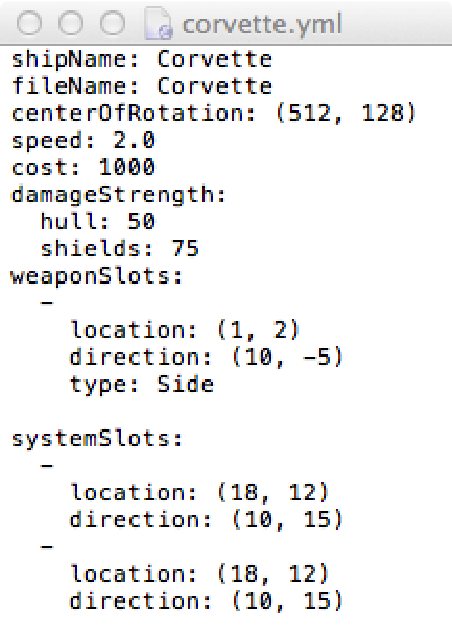
\includegraphics{res/configuration/corvetteYaml.pdf}
    \caption[Example of a YAML configuration file]{Example of a YAML configuration file.}
    \label{fig:corvette-yaml}
\end{marginfigure}

The addon definitions are stored in YAML files in the resources directory. YAML was chosen as the file format due to its focus on human readability. Other serialisation formats, such as XML and JSON, were considered, but were discarded in favour of the combination of brevity and readability afforded by YAML. When the game is launched, the resources directory is scanned for YAML configuration files and the data is loaded into memory. Adding new instances of models only requires adding a new YAML file to the appropriate directory, and configuring existing ones is as simple as editing a text file. Figure~\ref{fig:corvette-yaml} shows the corvette ship type defined in YAML.

\clearpage\section{Configuration}

% defining weapons, systems, ship classes, and fleets externally.
% information defined in yaml
% 

This section describes the method used to defines the various weapons, systems, ship classes, and fleets.
For simplicity, The weapons, systems, ship classes, and fleets will be referred to as Addons.
The reason for this name is that to add a new weapon, system, etc should be very easy from a development point of view.

Their were two options for this: defining the Addons within the code, or defining them in external resources and loading them in at runtime.
The second option is a cleaner and simpler design and allows new Addons to be defined without changing the code.

There are many data serialisation formats that are designed for this in mind, such as: XML, JSON, and YAML.
XML is highly verbose for both reading and writing, JSON requires braces for scope and quotes for any strings whereas YAML doesn't need either since it uses the white space for scoping and strings don't need quotes.
YAML is also designed to be human readable and writable, which would make manually creating and editing these Addons very easy.

It was important that new Addons should be discovered by the game when it loads, i.e. it would search for them in a given directory.
It would make the logic a little more complex but would make the interactions with the Addons very simple.
If you wanted to add an Addon simply add the a new yaml file to the correct directory, if you wanted to edit an Addon simply find the yaml file and change what values you wanted.
Unfortunately deleting Addons is not so simply, because some Addons will have dependencies on other Addons, for example a fleet may use a certain ship class, and if that ship class was deleted, that fleet would no longer be usable.
Making the deletion of Addons simple was considered, but decided against it because it would require disabling all Addons that had a dependency on a deleted Addon. This wasn't a clean design hence it is typically assumed that either no Addons are deleted or that the user knows what they are doing.
An example of a ship class defined in yaml is provided in Figure \ref{fig:configuration:corvetteYaml}


\begin{marginfigure}
	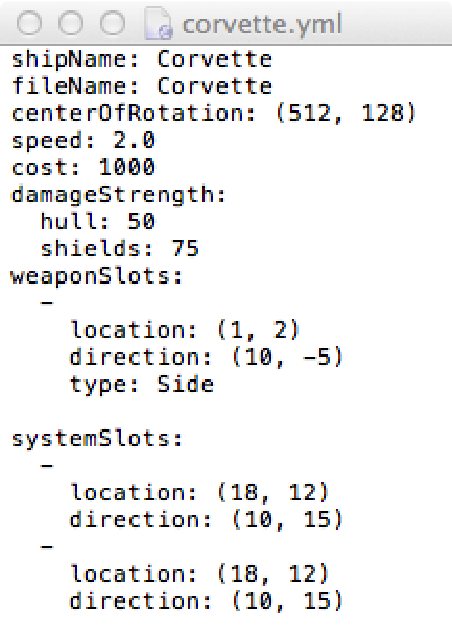
\includegraphics{res/configuration/corvetteYaml.pdf}
	\caption{
	example of ship class defined in yaml
	}
	\label{fig:configuration:corvetteYaml}
\end{marginfigure}



\clearpage\section{Resources}

\begin{comment}

what are resources

how they effects the game

for each resources:
  - what it's used for

\end{comment}

The resources represent the currency of the game. The player's access to resources can dramatically effect hit chances of winning a battle.

Each resouces has a unique purpose in the game, requiring the player to change strategy dependending on the type and quantity of resources the player has access to.

The three resources are:
\begin{itemize}
\item Fuel
\item Metal
\item Anti-Matter
\end{itemize}

% describe how their are gained (from planets)
Each planet on the map will have a supply of resources. 
The quantity of resources on each planet will vary, but will relate to the planet's type.
When that planet is captured, it will provide a constant trickle of its resources to the player.
For instance if a planet has the following resources:
\begin{description}
\item[Fuel]: 1
\item[Metal]: 2
\item[Anti-Matter]: 0
\end{description}
And is captured by player 1, then every minute, they will receive 2 metal from the planet, and 1 fuel. 
The planet will continue to supply the player with resources until the game ends or another player captures the planet.

% describe how the ship has access to the resources
Each ship will have its own cache of resources on board.
When the ship is near one of it's planets, It will have access to resupply from the player's stockpile. The ship's resource cache will automaticaly refill when near the player's planets. 
Larger class ships have bigger resource caches, and therefore can last longer before needing to resupply (subject to resource consuption).

When a group of ships leaves the safety of its own planets, and starts entering battles, their resource supplies will eventually become empty unless they return to one of their planets. 
If the group of ships continue to battle without resources they will eventually sustain damage to hull and will be more likely to loose the battle.
When a battle takes place within proximately to the player's planet, that player will have the benefit of a constant resupply of resources to the ships in battle. For the other player to win that battle they would need to do so before ship's resources start to dwindle.
This gives the defending player the advantage of endurance, being able to last a battle much longer.


\subsection{Fuel}
When a ship's shields are less than 100\%, Fuel is used by the ship to replenish the ship's shields.
The rate that the ship's shields are regenerated is dependent on the ship class, not the quantity of the ship's fuel cache.
If the ship runs out of fuel, it will stop regenerating its shields.

\subsection{Metal}
When a ship's hull takes damage, the ship is able to repair it on the go with the use of Metal onboard.
The ship will continue to drain it's supply of metal repairing the ship until it has full health again or its metal cache runs out.

\subsection{Anti-Matter}
The rarest of resources, is used as ammunition for a ship's most powerful weapons.
These weapons can only fire if the ship has Anti-Matter on board.
This reason can easilly swap the tide in battle.
\clearpage\section{Planet Capture}
<please insert shizzle here>
\clearpage\section{Artificial Intelligence: Orders, Goals, and Plans}
\label{sec:ai}

A sophisticated artificial intelligence (AI) system was highlighted as one of the major
functional requirements for the project. The plan was to use the AI to take high
level orders from the player and convert them into a detailed plan for individual
ships to execute. In this way the player would direct the overall strategy of their
fleet, but without actually captaining the individual ships. This would reduce the
amount of micromanagement a player has to undertake and increase the sense of realism
--- the admiral of a real fleet is unable to directly control individual ships under
their command. This plan for a high level AI was seen as one of the larger challenges
that the project would face.

Artificial intelligence can often be a make-or-break factor in determining the success of
a game.\citepage{rabin2002}{page 3} Without a convincing intelligence system, a game can
quickly become infuriating to play. This is because a human player expects any computer
controlled components to behave sensibly. In some cases well known algorithms exist that
enable `intelligent' behaviour to be implemented relatively easily, for example the use
of the A* search algorithm for pathfinding. However, higher level intelligence systems
are much more challenging. A system capable of creating and executing quality plans
from abstract orders is going to be one of the hardest components to implement.

As well as providing an entertaining experience an AI system must also be efficient.
There cannot be large delays between the user giving an order and it being carried
out. Any planning algorithms have to run quickly otherwise the lag in feedback will
detract from the realism of the game. An inefficient AI system could also stop the game
from running smoothly --- which is of great importance for a real-time strategy game.
This would lead to a poor user experience causing people to stop playing the game.
For these reasons, careful thought was put into designing a system that could fulfill
the important requirements for a successful AI system.

The AI framework that was implemented in Project Serenity is based on a planning
hierarchy. At highest level are orders, such as move to a given location or capture
the specified planet. These orders are under the control of the player, but it is
the job of the AI system to plan a series of actions to achieve them. The first step
is to convert the order into a goal. There is mostly a one-to-one mapping between
orders and goals, for example "OrderMove" maps to "GoalBeAt", however this layer of
abstraction allows the AI to choose unrelated goals if the current order is impossible
or would result in the needless loss of a ship. The goal is then decomposed into a
plan which is a series of actions that are performed to complete the current goal
(and hopefully fulfill the current order too).

The current planning cycle for a ship is as follows:

\vspace{-0.5em}
\begin{listing}{list:planning}{Planning cycle pseudocode}{Pseudocode for the AI framework's planning cycle.}{}
\end{listing}\vspace{-1.5em}

\begin{tabbing}
{\bf if} the current plan is empty {\bf then} \\
\quad{\bf if} the current order is complete {\bf then} \\
\quad\quad Reset the ship's order to "OrderNone" \\
\quad\bf else \\
\quad\quad $g \leftarrow$ create goal from the current order \\
\quad\quad $p \leftarrow$ create a plan from the new goal, $g$ \\
\quad\quad Update the ship's goal and plan with $g$ and $p$ \\
\quad\bf fi \\
\bf else \\
\quad{\bf if} the first action in the current plan is complete {\bf then} \\
\quad\quad Remove the action from the head of the ship's plan \\
\quad\bf else \\
\quad\quad Perform the action at the head of the ship's plan \\
\quad\bf fi \\
\bf fi
\end{tabbing}
\noindent
This planning cycle runs every server tick so that all ships in the game can
continuously formulate and update their goals and plans.

An improvement to the planning cycle would be to add in periodic replanning steps.
This would allow a ship to change its plan if the world around it changes, for example
to disregard an order to capture a planet if it is guarded by multiple enemy ships
and there is no friendly support in the area. In the current implementation this is
done on a bit of an ad-hoc basis instead of being formalised into the planning loop.
For example, the code that implements the action to move to another ship will check
if the target ship is still near to its location when the plan was originally formulated.
If the target ship has moved too far then the current plan is scrapped so that a new
plan can be constructed.

\subsection{Targeting Enemy Ships}

As well as constructing a planning framework for executing player given orders,
it was necessary to build some systems to carry out intelligent actions outside
of the usual planning loop. One such example is that of targeting enemy ships to
attack. As a ship moves about the sector it will fire upon any enemy ship that
it encounters. However, if there are multiple ships in the vicinity then it is
necessary to select which to target as it may not be possible to attack all of
them at once. A clever targeting system had to be devised to solve this problem
in an effective manner.

The first step is to generate a list of all potential enemy targets. This is a list
of all enemy ships that are in range of any of the ship's weapons. A list of
enemy ships to attack is selected for each weapon by taking the enemy ships that
would be attacked by the least number of other weapons as well. This method of
target selection means that a ship will spread its attacks out to hit as many
enemy ships as possible.

This pattern of list generation and selection fits the one described by John Hughes
very well.\cite{hughes1989whyfp} This is one of the reasons why the Project Serenity
team found Haskell to be highly adept for programming AI algorithms. The separation
between the potential target list generation and the selection from the list also means
that it would be very simple to modify the selection strategy. For example, a
possible enhancement to the game would be to allow players to configure a targeting
strategy for their fleet which would focus attacks on the weakest enemies.

%% todo: Fix 3.6 captions when jon and vic are done

\clearpage\section{Ships, Spacelanes, and Path Finding}
\label{sec:pathfinding}

The specification made it clear --- by the way weapons and navigation between planets was to be structured --- that ship motion needed to be relatively detailed. It is no use having a weapon that can be only used in one arc if ships could instantly pivot on the spot. Instead it was desired for ships to move as large objects with a great deal of momentum, with large turning circles and ponderous movements. However it would be undesirable for the motion of ships to be too realistic, as it would make the game needlessly difficult and confusing. A real object undergoing acceleration in space could of course, accelerate essentially indefinitely (until it was nearing the speed of light) but would need to take an equal amount of time to decelerate to stop again.

\begin{marginfigure}
	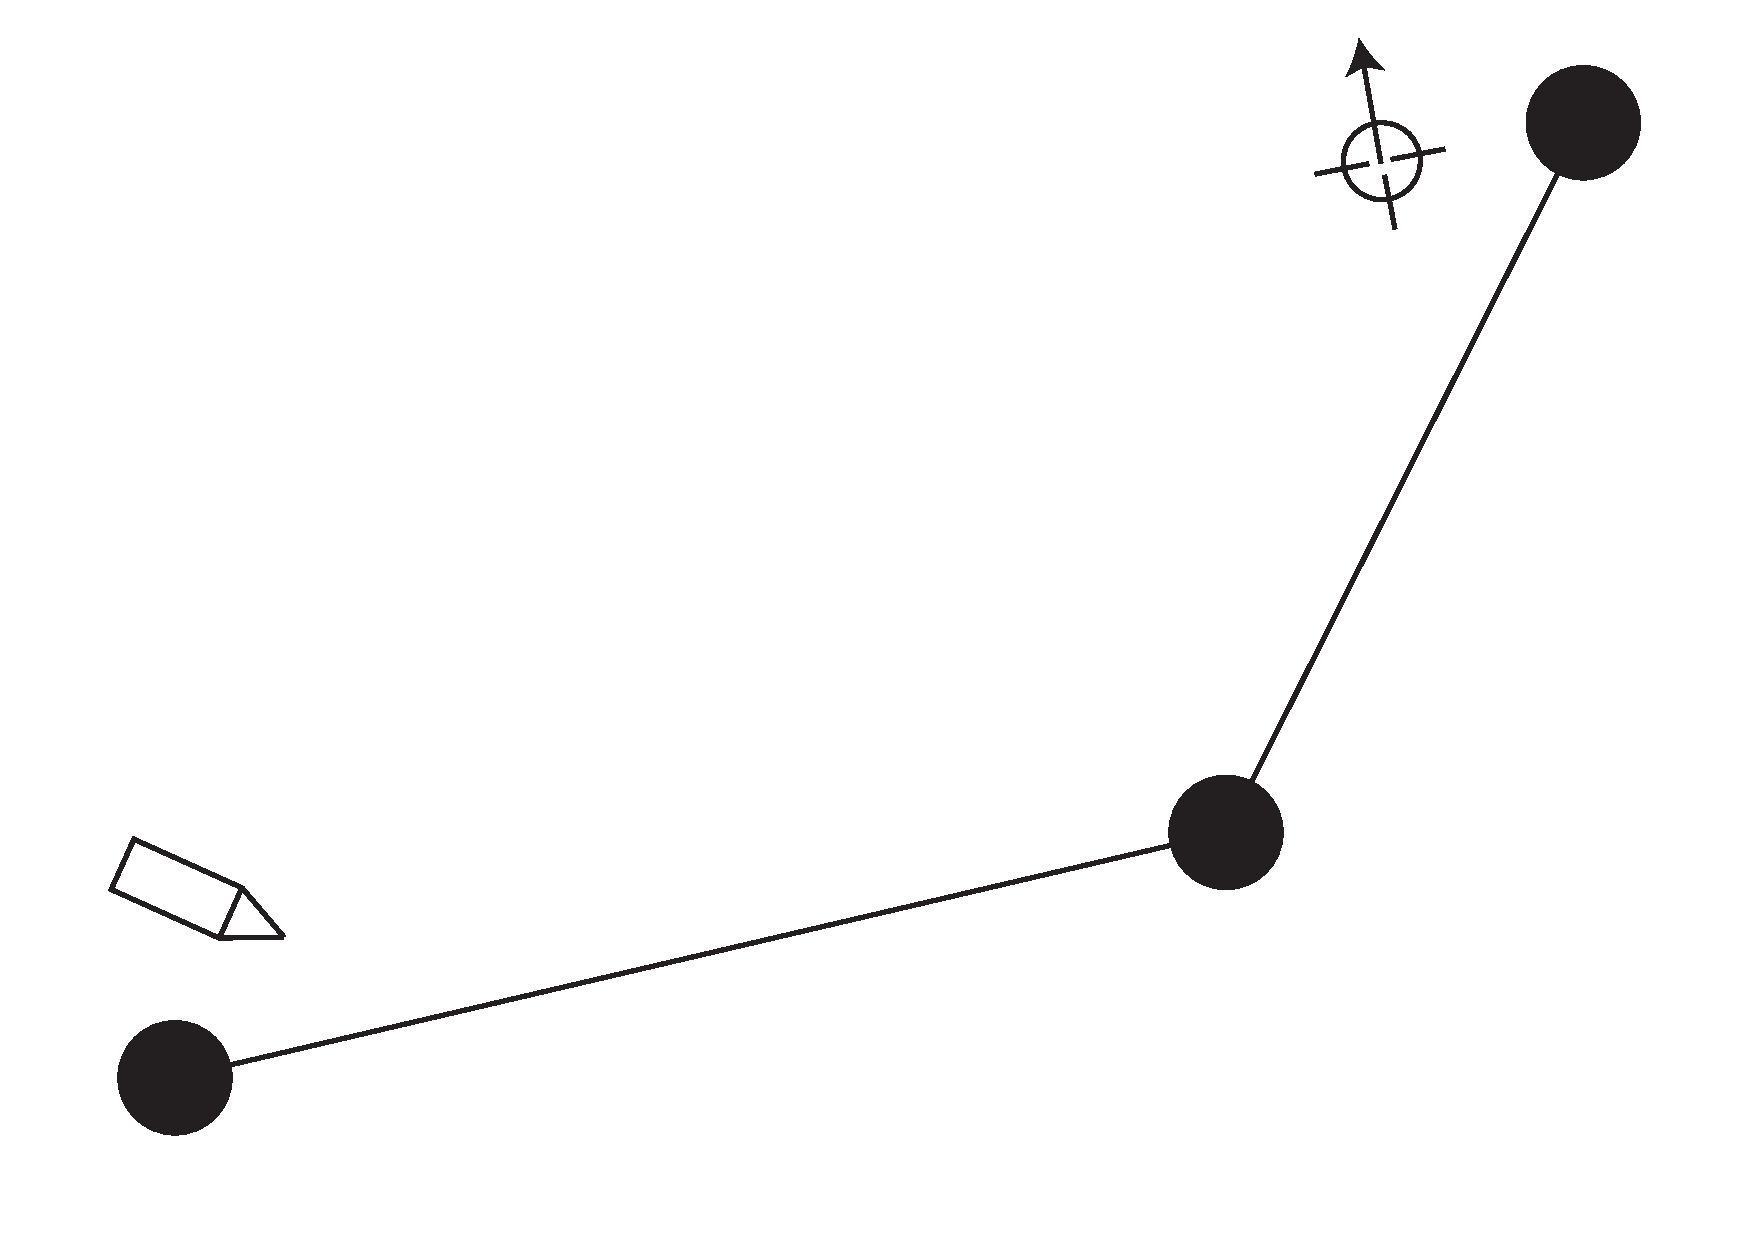
\includegraphics[width=20em]{res/pathfinding/spacelanes}
	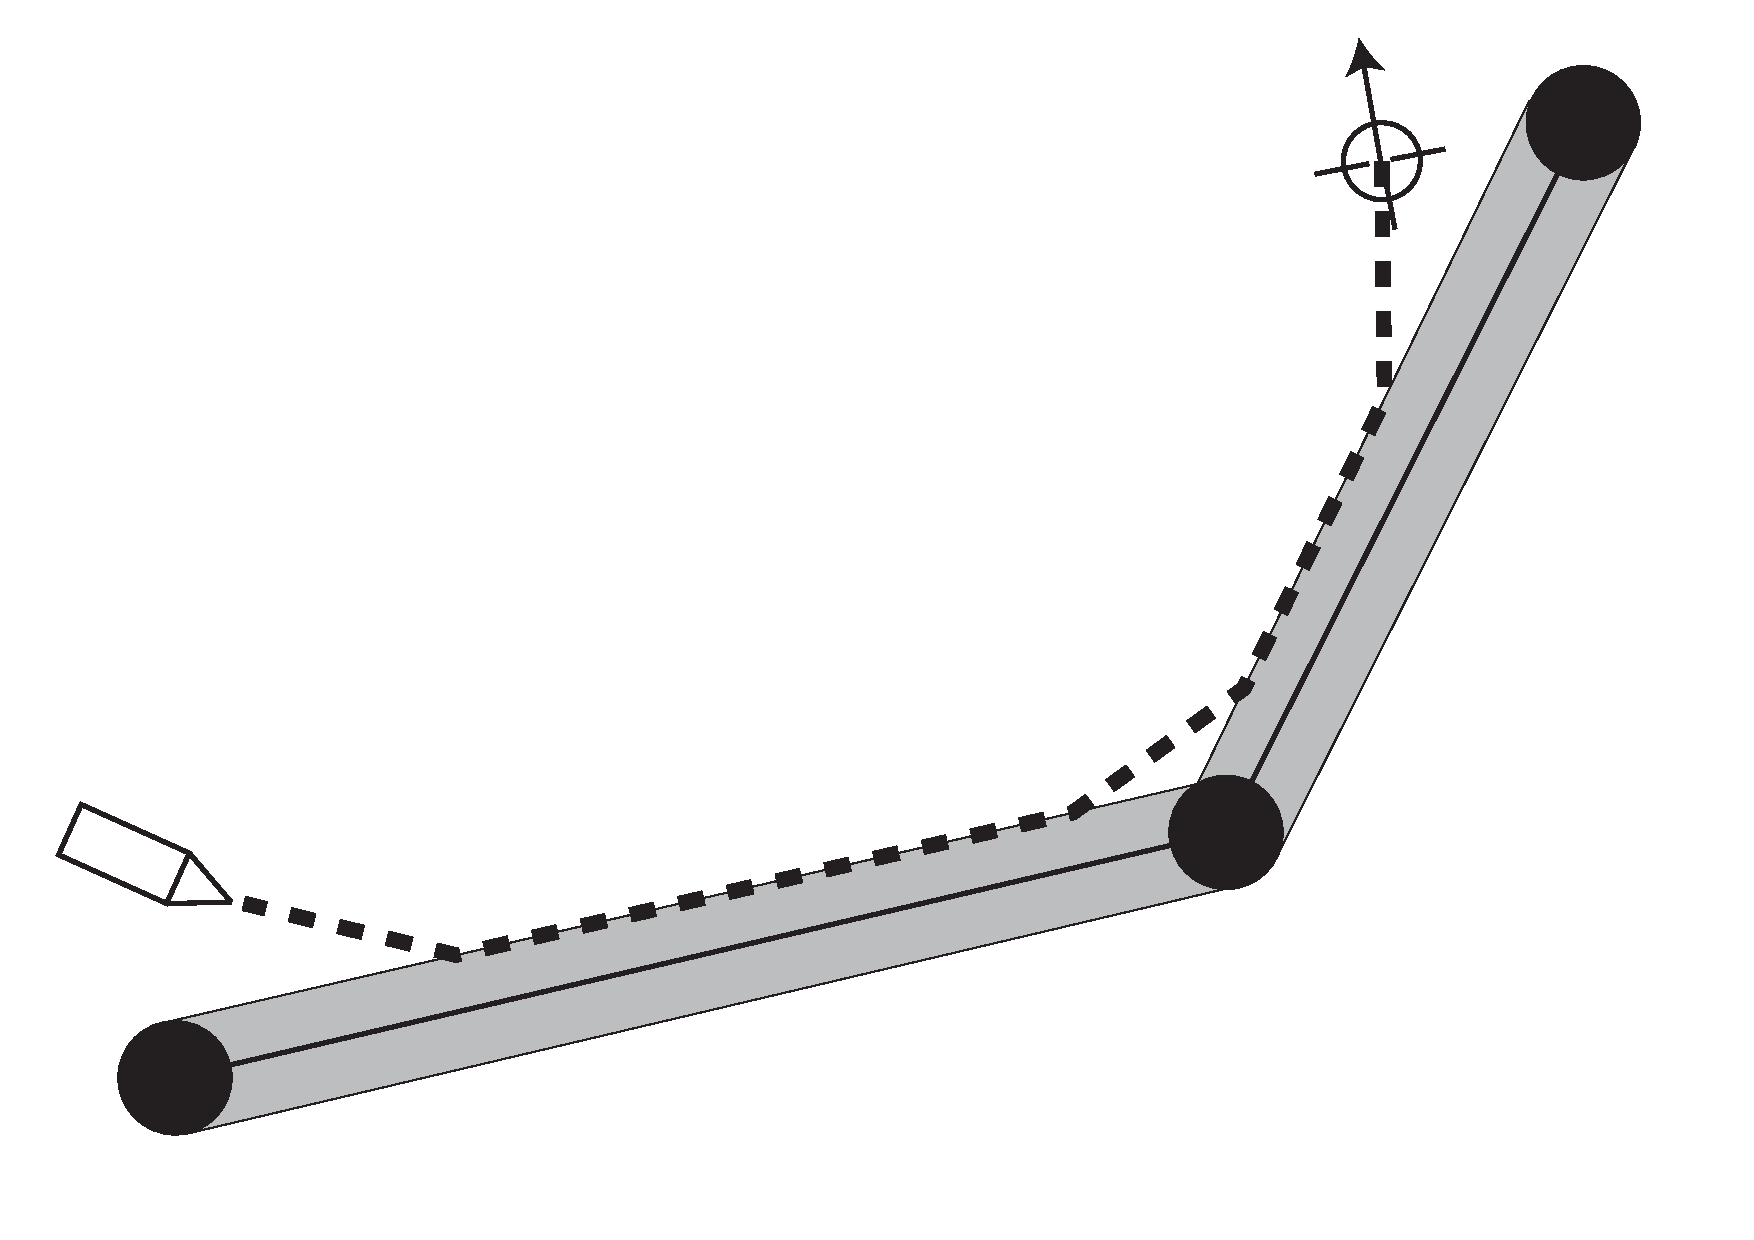
\includegraphics[width=20em]{res/pathfinding/spacelanes_ray}
	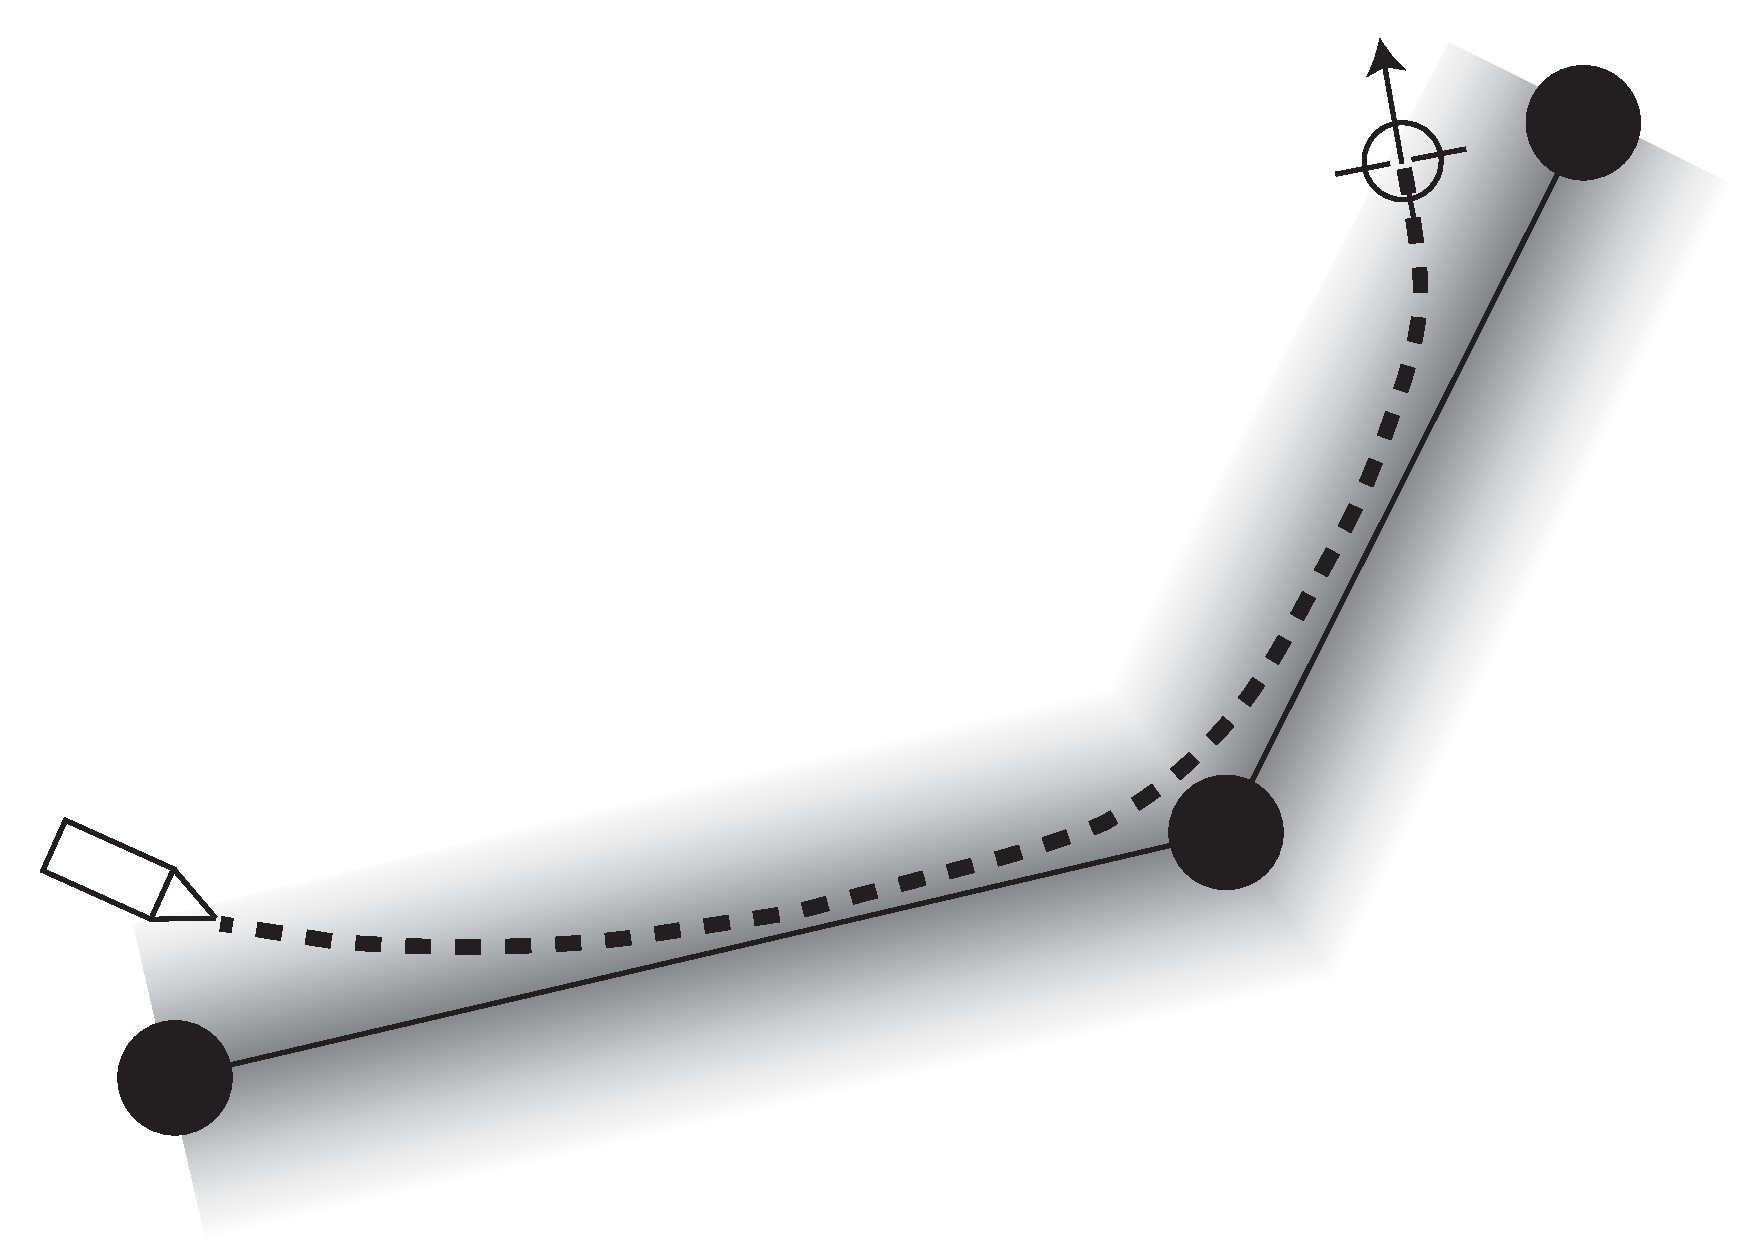
\includegraphics[width=20em]{res/pathfinding/spacelanes_field}
	\caption[Illustrations of different models for a path between current location and target utilising a spacelane]{Illustrations of different models for a path between current location and target utilising a spacelane.}
	\label{fig:spacelanes}
\end{marginfigure}

Intimately related to these questions is the precise nature of the \emph{spacelane} mechanics. Spacelanes between planets were introduced into the game in order for the otherwise empty space between planets to have some strategic topology, the idea being that the spacelanes can be traversed much more quickly than empty space. and so control of the lanes are vital to a successful strategy. Many different models were discussed for this mechanic during design meetings, both from the point of view of the in universe explanation, and the precise way in which the game would implement it. Initial ideas on the physical mechanism of the spacelane was that they conferred an additional optional acceleration: i.e. that if a ship is approximate to a lane it could opt to undergo greater acceleration than a ship far from a lane. But as mentioned, accurately modelling acceleration in space is somewhat contrary to the gameplay aspirations of the design. 

A simpler mechanic for ships that was considered to be more suitable, is for them to have a top speed that they could reach relatively quickly; but for them to still have large turning circles. This makes their motion more similar to naval ships engaged in warfare. The interpretation of the spacelane in this model cannot be simply a gain in acceleration as this confers little benefit. Instead it is clear that the spacelane must confer an addition to top speed. A possible physical interpretation of these behaviours is that the ships are moving in some kind of ether with friction, and so will reach a terminal velocity. The spacelane is then an area with an artificially induced lower density of ether.

Another fundamental question about the nature of the spacelane is whether its effects are immediately felt at full strength at a certain distance from it, or whether they fall off related to distance. the former is most definitely simpler, but the latter feels more natural as a mechanism. Figure~\ref{fig:spacelanes} shows the difference in the shortest paths that these approaches may generate, discounting the additional issue of ship turning.

\subsection{Algorithms for Pathfinding}
% physics hard
% bezier (not trivial)
% flow fields

Physical simulation of a large mass moving and turning in space was the initially preferred implementation method, but it became increasingly clear that this was going to be difficult both from an implementation and a user perspective. And while modelling the spacelane as having a continuous, field like nature, it was not at all clear how this would be achieved. It was decided to instead merely approximate the desired behaviour using bezier curves.

\begin{marginfigure}
	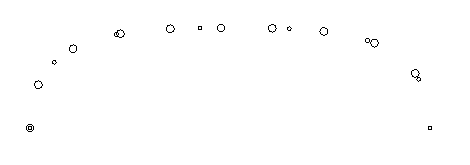
\includegraphics[width=20em]{res/pathfinding/bezier}
	\caption[Bezier path at regular intervals]{Bezier path at regular intervals (small circles) and the same path after having been reparameterisated by arc length (large circles).}
	\label{fig:bezier}
\end{marginfigure}

Over the Christmas break the code for a ship moving between two arbitrary points and headings was developed. Coding bezier paths themselves was not difficult, but moving an object continuously along one at a constant speed was much more complicated than expected. The accurate solution of this problem is called reparameterisation by arc length, and requires a solving a differential equation, but the method eventually used in Serenity was a numerical interpolation. Results are shown in Figure~\ref{fig:bezier}.

\begin{marginfigure}
	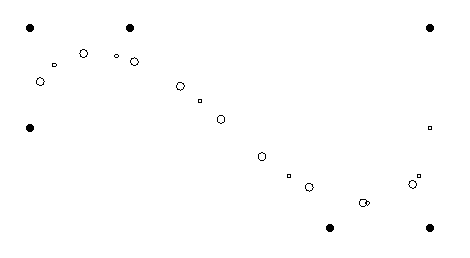
\includegraphics[width=20em]{res/pathfinding/bezierpath}
	\caption[Bezier path at regular intervals]{Bezier path at regular intervals (small circles) and the same path after having been reparameterisated by arc length (large circles).}
	\label{fig:bezierpath}
\end{marginfigure}

Even with the ability to move a ship smoothly along a given path, the selection of the path still required some considerable thought. An example of the control points generated for a move is shown in Figure~\ref{fig:bezierpath}.

\subsection{Applying A* to a Sector}
% what is the problem
% why this is no trivial problem
% Why A*

Applying a pathfinding algorithm to a sector has two stages: generating a graph which represents the sector, and running the algorithm that traverses the graph to find the shortest route to the destination. The algorithm chosen for the second stage is A* because it will always find the optimal solution (assuming the heuristic is admissible) and, if an efficient heuristic is used, then it is very fast too. However, the difficulty of using A* is that it requires a discrete graph to navigate, but the sector is not discrete as ships can move anywhere within it. The planets and spacelanes provide some points of reference, but they do not restrict the movement of the ships. Therefore, it is necessary to build a discrete graph from the sector model during stage one.

Just using the planets as nodes connected by edges of spacelanes does not work since the ships can go into other areas of space not covered by such a graph. Advanced techniques such as constructing a navigation mesh or a waypoint graph do not really apply in this situation since there are no obstacles for graphs to be built from. So, the solution was to take the simplistic graph generated only from the planets and spacelanes, and then add extra nodes and edges where appropriate. Extending the graph with these extra nodes was the difficult problem that had to be solved.

\begin{figure*}[h!]
	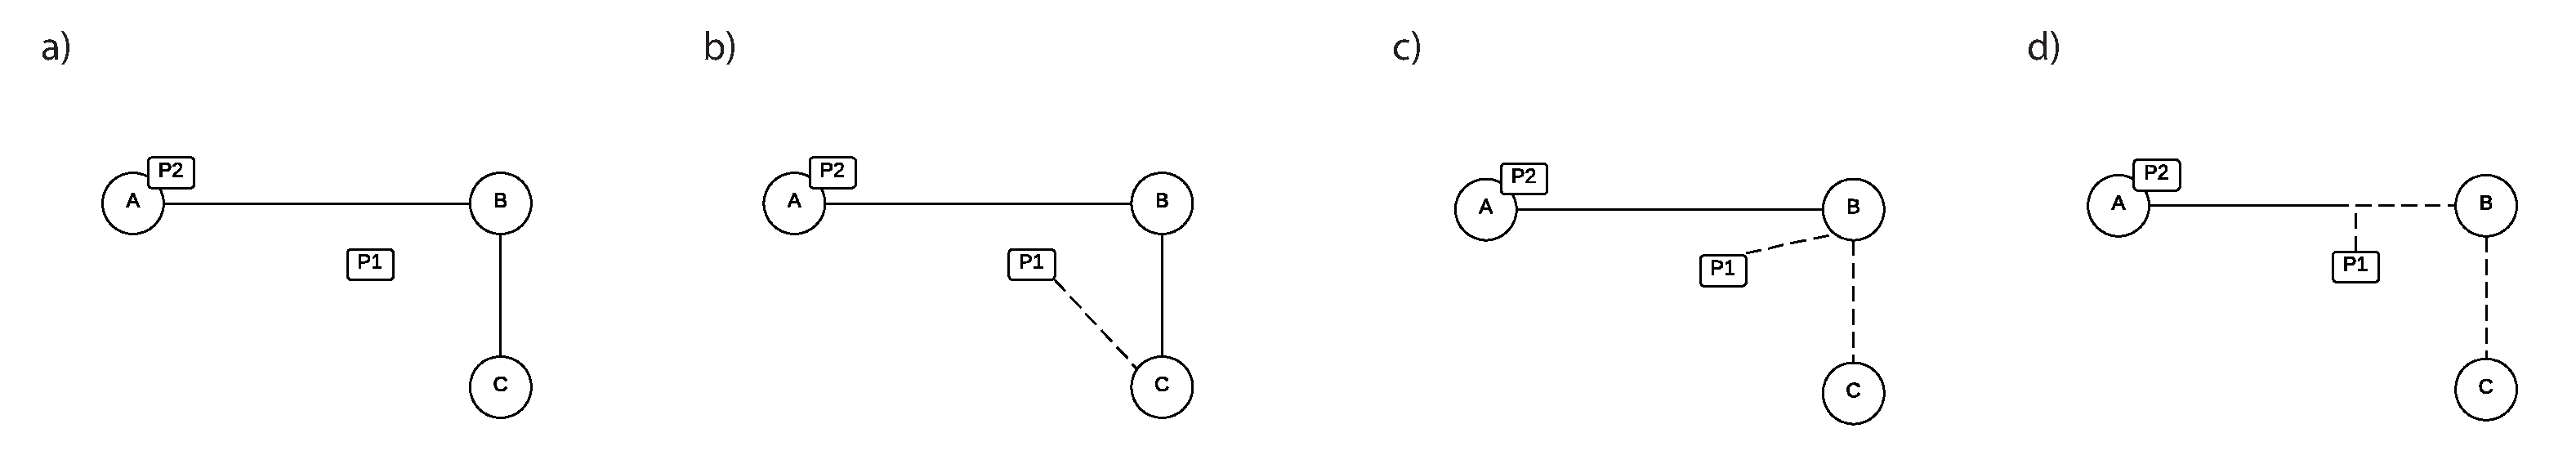
\includegraphics{res/pathfinding/PathFindingExample.pdf}
	\caption[Potential ship routes]{Potential routes a ship could take to reach its destination.}
	\label{fig:pathfindingexample}
\end{figure*}

First a typical ingame situation was taken to be analysed for the possible routes that a ship could take. Figure~\ref{fig:pathfindingexample} shows such a scenario. Figure~\ref{fig:pathfindingexample} (a) shows the location of two ships, $P_1$ and $P_2$, and three planets, $A$, $B$, and $C$, connected by spacelanes. If both ships want to reach planet $C$ then it is obvious which route $P_2$ will take, it can travel along spacelanes from $A$ to $B$ to $C$. However, there are three different possibilities for ship $P_1$:

\begin{enumerate}
	\item Go directly to planet $C$, shown in (b).
	\item Go to the closet planet, $B$, and then follow the spacelane to $C$, shown in (c).
	\item Travel to the nearest spacelane, between $A$ and $B$, and then follow the spacelanes to $C$, shown in (d).
\end{enumerate}

Travelling across open space is always going to be considerably slower than using spacelanes, so option one can be immediately be discarded as suboptimal. However, how fast are spacelanes? Is it best to greedily use spacelanes as much as possible or is it sometimes faster to travel a little longer through open space to reach a spacelane closer to the destination. Spacelanes have a multiplier effect on the speed of a ship so that a ship travelling along a spacelane speeds up $x$ times compared to its usual speed, where $x$ is a parameter defined by the sector model.

Suppose that $x$ is very large or infinite then travel along spacelanes with be almost instantaneous. Under these circumstances option three will be the optimal route since the least time is spent travelling off of spacelanes. However, for a lower value of $x$, option two will be optimal since the reduced distance to reach planet $B$ outweighs the benefits of the spacelane. Therefore, it is obvious that the heuristic cost function used by A* must take the multiplier effect of the spacelanes into account:

\begin{equation*}
	cost = \frac{distance}{speed \times multiplier}
\end{equation*}

Where the $distance$ between two nodes is simply the Euclidean distance. Using this cost function it becomes easier to find a good route by adding `virtual nodes' to the graph on nearby spacelanes and then using the A* algorithm to compare the costs of this extended graph. For example, in the scenario shown in Figure~\ref{fig:pathfindingexample} a virtual node is added to the spacelane between $A$ and $B$. This suggests a simple set of rules for adding new nodes:

\begin{enumerate}
	\item If the start point is in open space then add a node at the closest point on the closest spacelane
	\item If the destination is in open space then add a node at the closest point on the closest spacelane
\end{enumerate}

\begin{marginfigure}
	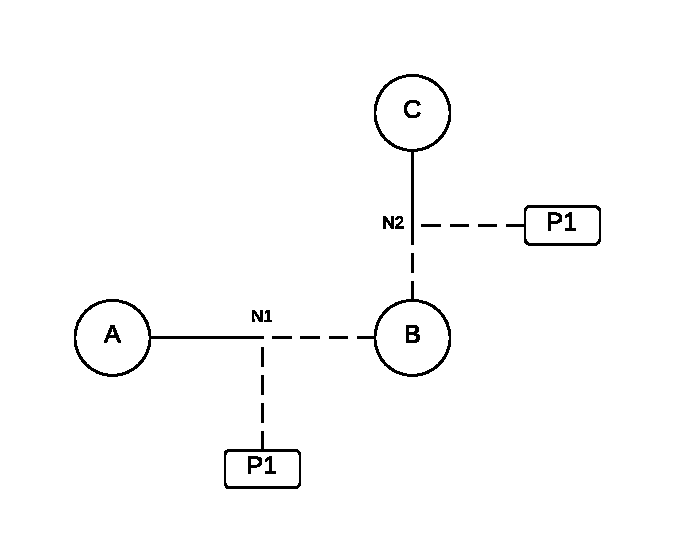
\includegraphics{res/pathfinding/PathFindingSector3.pdf}
	\caption[Adding nodes to the nearest spacelanes]{Adding nodes to the nearest spacelanes.}
	\label{fig:addingnodes}
\end{marginfigure}

For example, Figure~\ref{fig:addingnodes} shows how two nodes are added at $N_1$ and $N_2$ if a ship wants to go from $P_1$ to $P_2$. The graph is then completed to make all of the sensible routes connected. Using the same example from Figure~\ref{fig:addingnodes} it means that edges will be added between the $P_1$ and $N_1$, $P_2$ and $N_2$, $P_1$ to $B$, $B$ to $P_2$, and so on. The A* algorithm, using the simple cost function, can then be applied to this fully connected graph to find the best possible route to the destination.

\begin{marginfigure}
	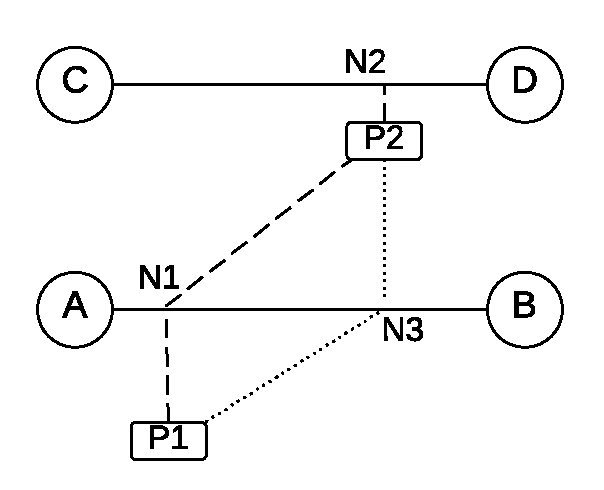
\includegraphics{res/pathfinding/NearestSpaceLaneUseless.pdf}
	\caption[The closest point on the closest spacelane is not always your friend]{The closest point on the closest spacelane is not always your friend.}
	\label{fig:uselessspacelane}
\end{marginfigure}

However, these two rules are too simplistic and will not provide the best route in all cases. Figure~\ref{fig:uselessspacelane} shows an example in which a ship wants to travel from $P_1$ to $P_2$. The current ruleset will add nodes $N_1$ and $N_2$ since they are the closest points on the nearest spacelanes. However, it is actually quicker to travel via $N_3$ than it would be to go straight from $N_1$ to $P_2$. There are just too many possibilities for quicker routes as the edge cases keep on building up. Therefore, it was decided to use a brute force solution that involves adding nodes at regular intervals along the nearest spacelanes. The best added node may not match the optimal solution exactly, but it will be better than the majority of other options. Using brute force is also not a highly desirable technique, but it works fast enough for this use case for now as further designing would have been required to reach a better solution.

Now that a discrete graph has been generated to represent the sector it can be fed to the A* algorithm which will find an optimal solution for the graph it has been presented.

\clearpage\section{Rendering the Game}

% old assets
% ----------
% ships made to look very big
% many prototypes
% merging assets with code, dynamic color

% master copy of assets in dropbox under 4y project/laith/design

One very important aspect of the client program is rendering the current game state to a display for the user to interact with. Creating a picture of the game to display requires a number of graphical assets to visually represent the various entities and scenery that make up the game world. For Project Serenity all of these graphics were created from scratch using Photoshop and Illustrator. Figure~\ref{fig:assets} shows a selection of some of the assets that were created for different entities.

% TODO INSERT FIGURE OF PLANETS AND SHIPS
% full page on planets, full ships

% TODO Chat about the actual rendering process. Thoughts:
%
% * World coordinates: all entities are located in world coordinates and a view of the world is drawn in this way first
% * Viewport: the display is scaled and translated by the current settings stored by the client
% * Along with the actual world there is some extra GUI that helps the player understand the current state of the game:
%      - Minimap
%      - Currently selected entity

The client uses these assets to draw the sector and place each player's ships in the correct locations. This is done by placing the assets using world coordinates in the 2D space defined by the dimensions of the sector.

% TODO Talk about parallax because it's interesting? (Innovative?)

Another interesting piece of the rendering puzzle was to choose a colour as a unique visual representation for each player. This would be used to help players differentiate their ships from the enemy and to identify the planets that they own. A clever algorithm was used that would take a numerical player identifier and return a unique colour:\cite{ankerl2009}

\begin{equation*}
	colour(i) = HSV(i \times \phi^{-1} \mod 1, 1.0, 0.8)
\end{equation*}
\noindent
This function uses the HSV colour space using a fixed saturation and value, but modifying the hue to create equally bright and vibrant colours. The player's identifier, $i$, is used to step into the possible values for hue by multiplying it by the reciprocal of the golden ratio, $\phi$, modulo one. Due to the equidistribution theorem\sidenote{The equidistribution theorem states that the sequence $a, 2a, 3a, \ldots \mod 1$ is uniformly distributed when $a$ is an irrational number} this creates a sequence of colours that are evenly spread across the colour space. Using this method to generate team colours created visually pleasing colours that are suitably distinct from each other to be used for recognition.

\clearpage\section{Menus and a Splash Screen: The Front End}

\begin{itemize}
    \item Lots of screenshots!
    \item Explanation of menu system and splash screen, credits screen etc
    \item Discussion of some UI principles used
    \item mention sheen (GUI) framework from non-technical perspective (design / logic split etc).
\end{itemize}

\begin{figure*}[p]
	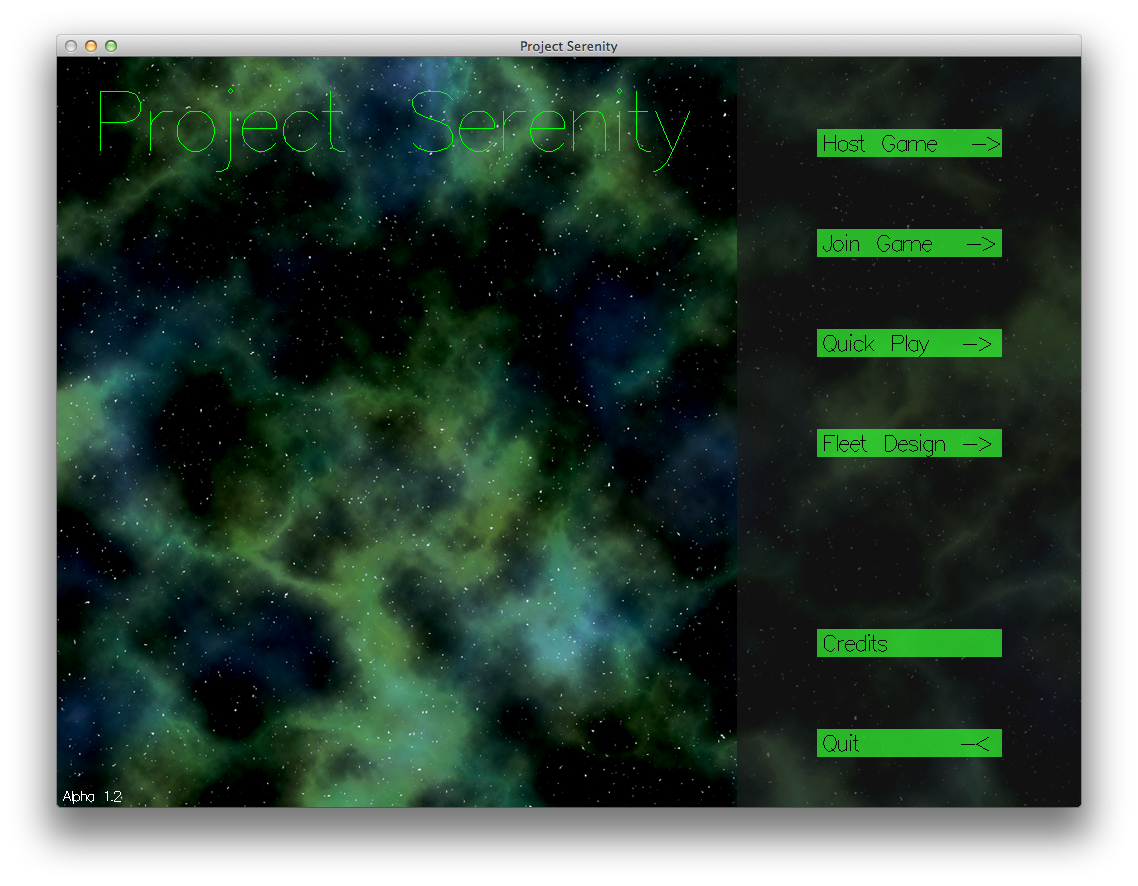
\includegraphics[width=15.5cm]{res/serenityscreens/01-mainmenu}
	\caption[Screenshot of the main menu]{Screenshot of the main menu.}
	\label{fig:mainmenu}
\end{figure*}

\begin{figure*}[p]
	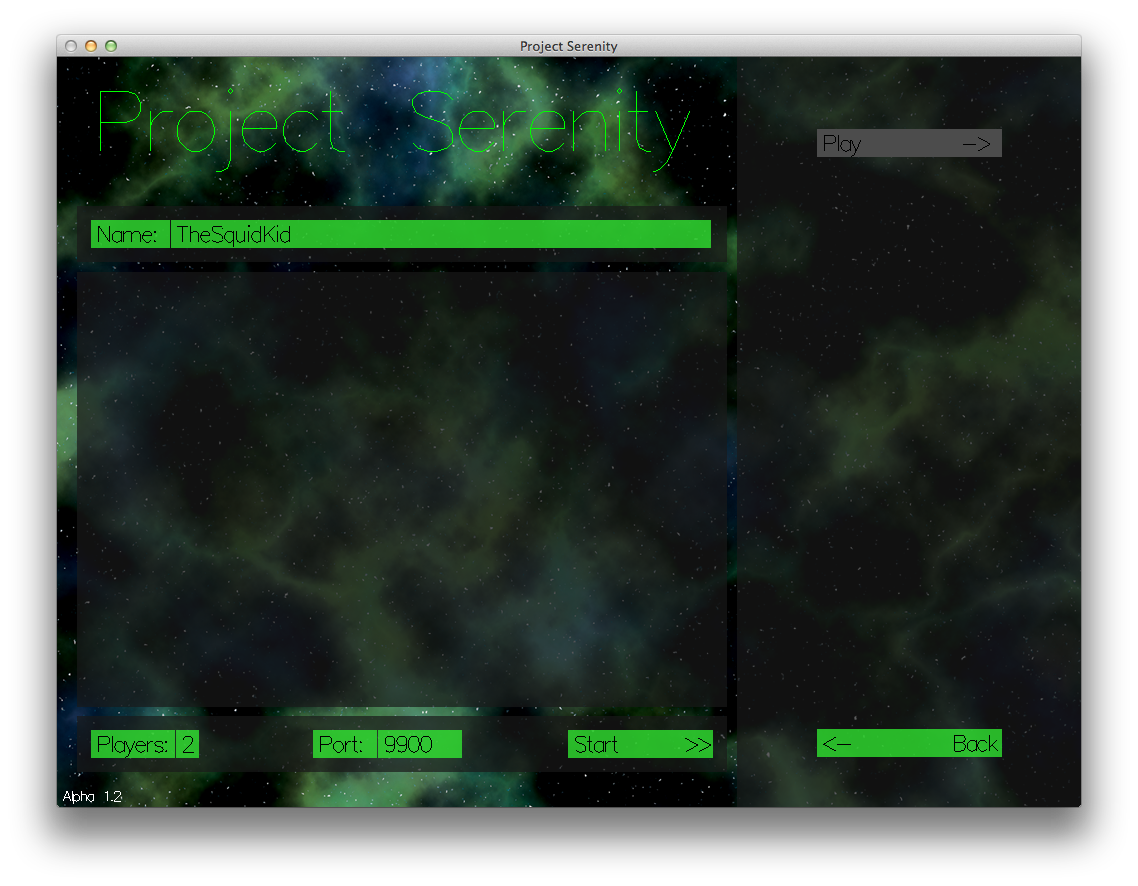
\includegraphics[width=15.5cm]{res/serenityscreens/02-host}
	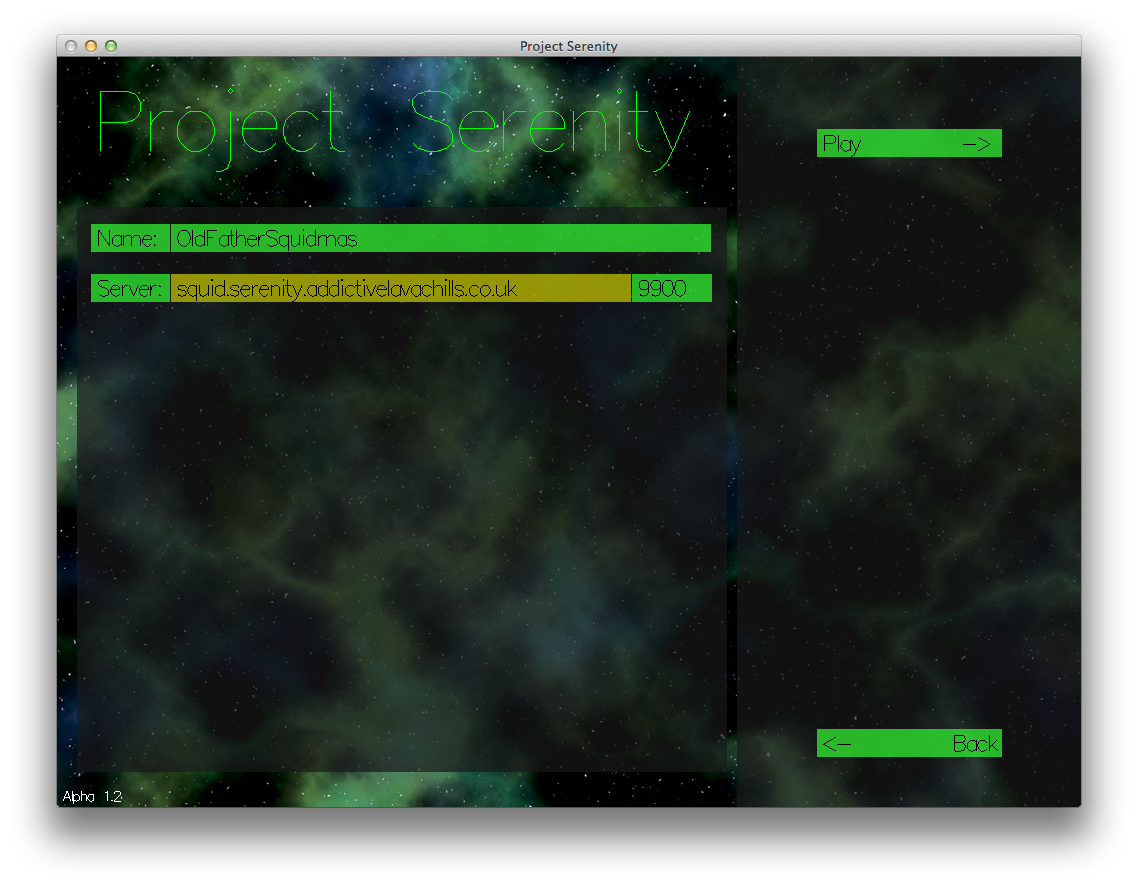
\includegraphics[width=15.5cm]{res/serenityscreens/03-join}
	\caption[Menus for hosting and joining battles]{Screenshot of the menus used to host and join battles.}
	\label{fig:hostjoin}
\end{figure*}

\begin{figure*}[p]
	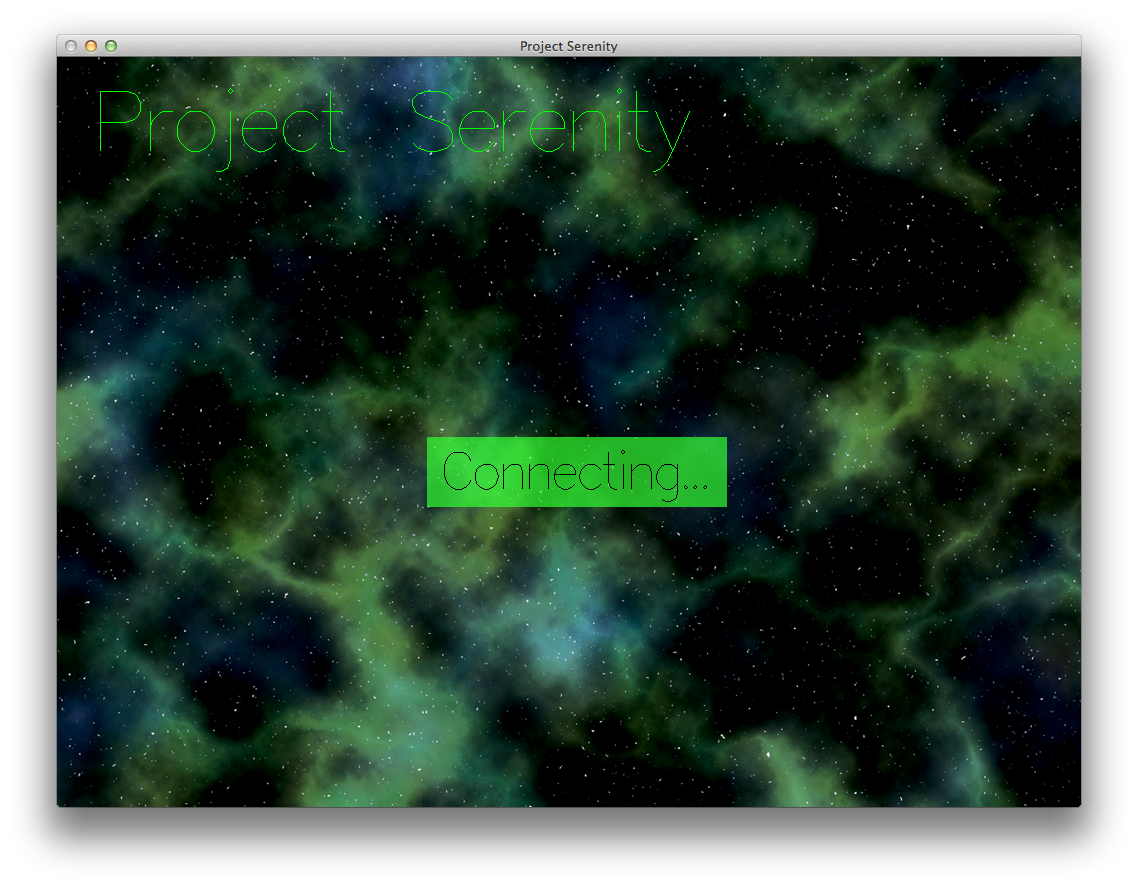
\includegraphics[width=15.5cm]{res/serenityscreens/06-connecting}
	\caption[Screenshot taken as a player connects to a server]{Screenshot taken as a player connects to a server.}
	\label{fig:connecting}
\end{figure*}

\begin{figure*}[p]
	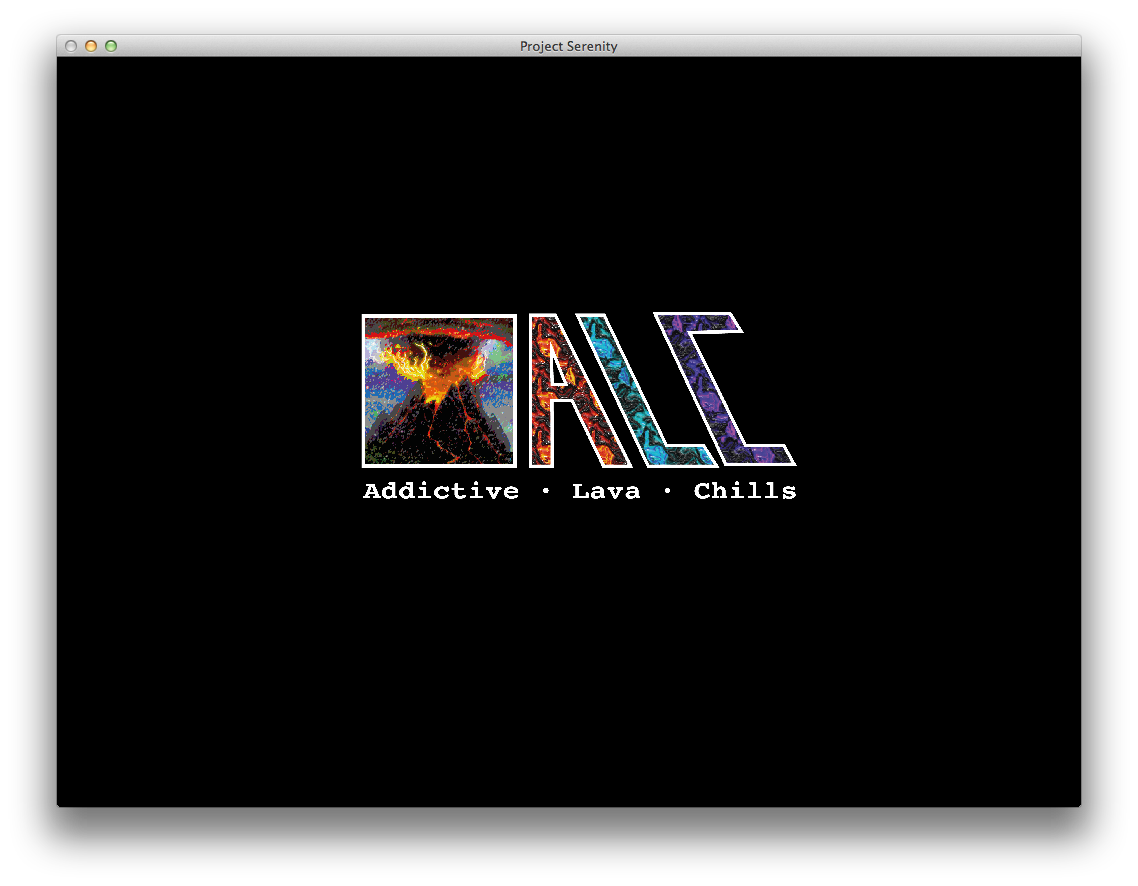
\includegraphics[width=15.5cm]{res/serenityscreens/07-splash1}
	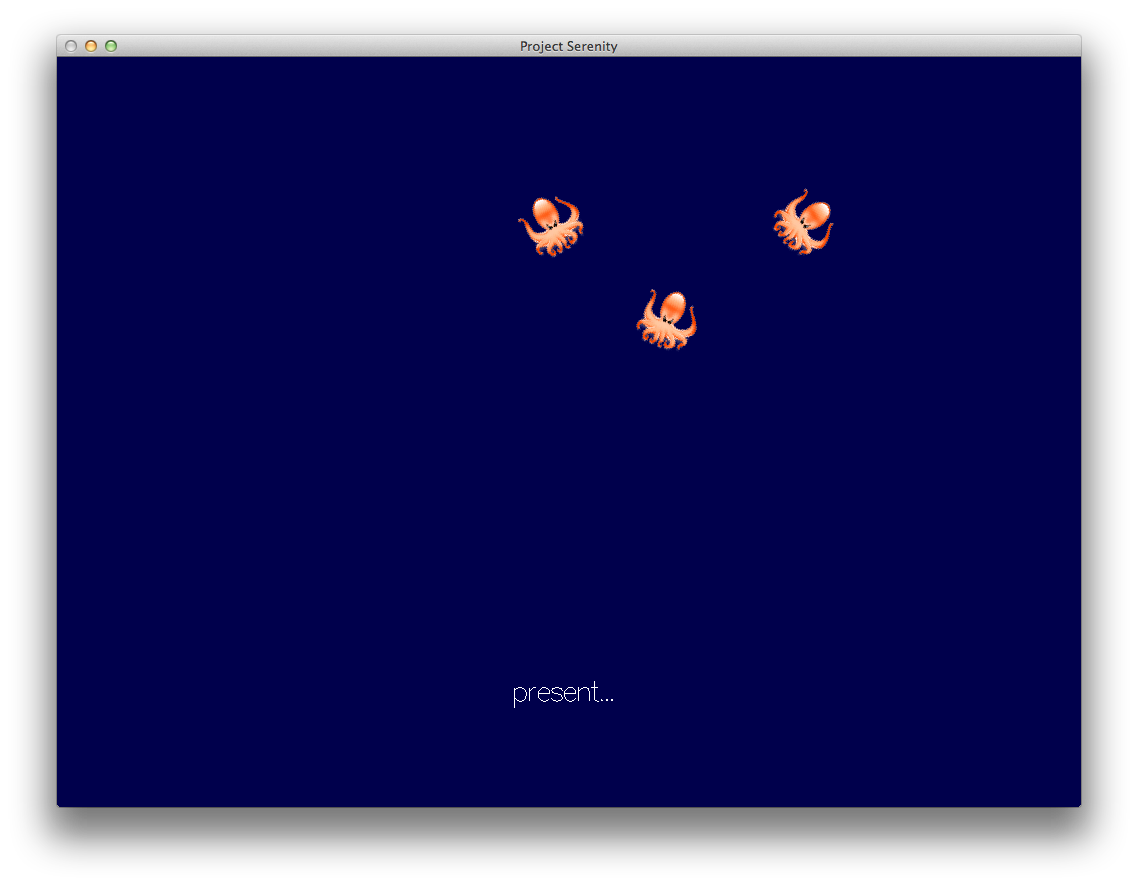
\includegraphics[width=15.5cm]{res/serenityscreens/08-splash2}
	\caption[Splash screens shown on launch]{Screenshot of the splash screens shown when the game is launched.}
	\label{fig:splash}
\end{figure*}

\begin{figure*}[p]
	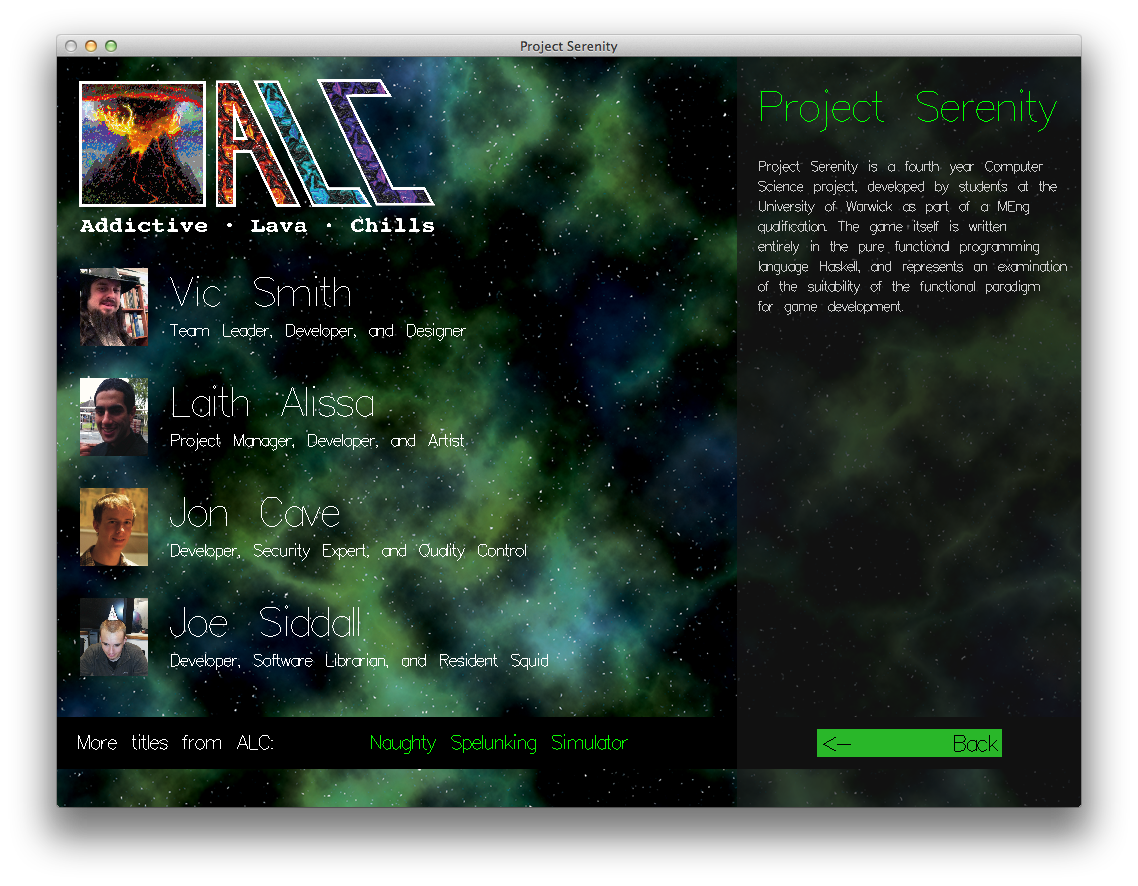
\includegraphics[width=15.5cm]{res/serenityscreens/05-credits}
	\caption[Screenshot of the credits screen]{Screenshot of the credits screen.}
	\label{fig:credits}
\end{figure*}


    
\begin{comment}

story boards:
  - client/server updates loop
  - graphics:
    - navigation
    - Paralex
  - GUI interfaces: 
    - Main Menu
    - credits
    - Game Play 
    - fleet design 
    - Results Screen
  - resources
  - planet capture
  - ship weapons arcs
  - model (sector, ship, etc)
  - AI concepts (PLAN/GOAL/ORDER)
  - path finding
    - A*
    - Bezier path
    - Flow fields
  - assets and configuration
    - assets
    - asset meta data
    - fleets
  - future work sections...
  - conclude (something)
  

\end{comment}

\begin{comment}
Revised layout?

* Client-Server Architecture
* Modelling the Game
* Configuring the Models
* Resources: The Currency of the Game
* Planetary Capture
* Artificial Intelligence: Orders, Goals, and Plans
* Ships, Spacelanes, and Path Finding
* Rendering the Game
* GUI (The End Product?)

\end{comment}


\begin{comment}

overall layout
--------------
game decisions
where we got to in spec
current state of game
lots of pictures

very little technical detail

lot of work on infrastructure at start



layout:
- laying the foundations:
    - got infrastructure sorted out:
        - network
        - overall glue
- alpha stage (Christmas):
    - demo stage
- leading beta stage:
    - messages/updates
    - better graphics
    - AI
- current state
- play testing and feedback
    - LIE we did lots
- future work(ryan's mum)


\end{comment}

\chapter{A Practical Guide to Haskell Game Development}
\label{ch:rd}
\containsfigures{The ALC Guide to Haskell Game Development}
\containslistings{The ALC Guide to Haskell Game Development}
%\containstables{The ALC Guide to Haskell Game Development}

\chapterepigraph{The designer of a new system must not only be the implementor and the first 
large-scale user; the designer should also write the first user manual\ldots 
If I had not participated fully in all these activities, 
literally hundreds of improvements would never have been made, 
because I would never have thought of them or perceived 
why they were important.
}{Donald E. Knuth}

\chapter[Introduction]{Introduction}
\label{ch:motivation}

\chapterepigraph{If you aren't sure which way to do something, then do it both ways and see which works better.}{John Carmack}

\newthought{Functional programming} (FP) has a long history, with its roots in the $\lambda$-calculus of Alonzo Church.\citefix[-1.5em]{church1932} One of the first functional programming languages was Lisp, invented by John McCarthy in 1958, which is still used today, over 50 years later.\citepage{reilly2003}{pages 156--157} Various languages have refined and extended the functional paradigm over the years --- probably the most notable as of now being Haskell, Scala, OCaml, F\#, and Erlang.

Despite the amount of time such languages have been available, use in industry has typically been far less than that of languages such as C, C++, and Java.\citepage[-2em]{odersky2010programming}{page 11} That being said, in recent years there has been increasing use of functional techniques and languages in certain areas. Erlang was designed for the development of highly fault tolerant telecommunication systems.\cite[-1em]{armstrong2007history} OCaml is used extensively by some organisations in the financial sector to create trading algorithms and other similar applications.\citefix[1em]{minsky2011ocaml} Scala is also increasingly popular, helped in part by its compatibility with the Java Virtual Machine (JVM) and object oriented design.

One of the often cited reasons against the use of functional programming in some domains is that of performance. This is due in part to mutable data structures generally being easier to represent on machine hardware; and it therefore being harder for functional compilers to convert the code into an efficient representation.\citefix{paulson1996ml} However, it is not a given that any program would run slower if written in a functional language: in some cases lazy-evaluation or compiler optimisations made possible by immutability can mean a program runs faster, plus advanced compiler techniques such as array fusion can lead to programs nearing the efficiency of hand-crafted C. And with modern machines getting ever faster, the domain of problems that require high levels of efficiency is getting smaller.

Performance problems alone cannot account for the fringe position of functional programming. The efficacy of the functional approach has been touted for many years,\sidenote{For example see \bibentry{hughes1989functional}.} yet it is still rare for mainstream projects to make any use of functional languages.

Instead of researching and discussing the theoretical advantages of the functional paradigm, this project will attempt to demonstrate the value of functional programming by utilising it in a problem domain that should pose a significant challenge that is not normally considered a `good' domain for FP. The chosen application for the project is a game.

\section{Why a Game?}

Game programming brings together a diverse range of computing areas. For example human interaction in real time, detailed graphics and animation, artificial intelligence / planning, networking, and various other dynamic elements.\sidenote{See \bibentry{crawford1984art}.} A game is also a tangible, sizeable piece of software, yet achievable for a four person group over two terms.

As well as demonstrating FP over a wide range of areas, a game also represents a serious business venture.\cite{essentialFacts2012} Computer games have been a huge industry for almost as long as personal computers have existed. Demand is high, and a vast amount of games are being continually developed, from triple-A ventures and big companies, down to indie companies and fan groups.

This project will certainly not be the first game ever to be developed in a functional language, nor is it likely to be the last. The project shall therefore not only deliver the finished game, but fully document the process --- explaining what went well and how the functional approach benefited the construction, as well as what proved challenging.

\section{Picking the Language}

There are several functional languages that would be suitable for this project, most of which have already been mentioned. Of these, the language chosen is Haskell. The reasons for this are outlined below.

\begin{description}
	\item[Concision] Haskell code is concise, yet readable. This is a very real advantage as it allows both for fast writing of code, as well as fast refactoring and maintenance. 
	\item[Purity] Haskell is a pure functional language, with all the advantages that gives. However side-effects and mutability are needed for real programs (especially games) and Haskell has excellent tools for solving these problems, via the IO Monad, State monads, etc. The `do' syntactic sugar makes Haskell one of the best languages for this.
	\item[Speed] Haskell has very good compiler support, and the Glasgow Haskell Compiler (GHC) is capable of producing highly efficient code. 
	\item[Type System] Haskell has a very advanced type system, which makes bugs and errors in refactoring easy to detect quickly. Automatic type inference allows for these advantages without the type system slowing down the programmer.
	\item[Testing] The purity of Haskell enables automated testing techniques not possible even in other functional languages. There are also well supported testing libraries available for both pure and impure code.
	\item[Community and Library Support] The Haskell community is very active and there are extensive libraries available for it. Due to Haskell compiling to C, most C system libraries have Haskell bindings. There are OpenGL and OpenAL, for example.
	\item[Familiarity] All members of the group have some experience with Haskell, and consider developing with it to be very enjoyable.
\end{description}

\section{Existing Systems}

To avoid confusion we shall consider separately research into functional programming for games, and what game we will actually make given current and historic trends in gaming.

\subsection{Existing research into Functional Programming of Games}

One of the most well known games written in a functional language (Haskell, as it happens) is \emph{Raincat}\sidenote{Source available online from \url{raincat.bysusanlin.com}.} written in Haskell and developed by Carnegie Mellon students in 2008. There is also a game company, \emph{ipwn studios}, who exclusively use Haskell for their products.\sidenote{See there website: \url{ipwnstudios.com}.} Despite this, there is little work on the academic research side that supports or opposes functional languages for games. 

There was a similar project in 2005 by Mun Hon Cheong, an undergraduate at the University of New South Wales;\cite{cheong2005functional} and though Cheong did manage to create a complete 3D game and gave detailed descriptions of some of the code techniques, the project did not provide a detailed insight into what exactly was effective, or challenging, about the use of a functional language.

The fact that an exhaustive search of the literature in this area revealed only a single undergraduate dissertation highlights the paucity of available research in this area, and coupled with the growing interest in functional languages for game development shows the case for this project.

\subsection{Existing Games}

Needless to say, the complete history of gaming, even if only restricted to computer games, would be too lengthy to examine here. The gaming industry has grown hugely since the early commercial computer game systems, in parallel with the huge developments in the capabilities of computers themselves. And while some games today are magnificent technical achievements with breathtakingly detailed graphics, sounds, and physics engines, there are many popular titles from indie game companies using only 2D graphics and simple engines enjoying success. It is not just the cutting edge of technology that can make a game fun.\sidenote{This is a complex issue. For a more complete treatment see \bibentry{malone1981makes}.}

In order to serve the purposes of the project, it will be necessary to create a game designed to compete in the current market. This doesn't mean it has to be as complete, complex, or technically sophisticated as a triple-A title, but it does have to be a game that, if fleshed out fully, would be considered fun and suitable for a small company or similar organisation to sell. Without this any conclusions drawn about the efficacy of the approach will not be sufficiently valid to developers.

For this reason it is worth briefly reviewing a few games --- some modern, some less so --- in order to identify what would be an appropriate brief for a game to help achieve the project's aims.

An early game that was hugely successful, as well as controversial, is \emph{Doom}, a first person shooter developed by John Carmack and John Romero of id Software and released in 1993. Doom was marketed using a shareware model --- the first third of the game being distributed for free, and the rest available for purchase. Doom represented a revolution in what was possible in a computer game, and is widely accepted as the game that popularised the first-person genre. The slickness of the graphics engine, the thought provoking levels and puzzles, the controversial satanic imagery, all contributed to Doom's success. But the arguably the greatest innovation with the most effect on future gameplay was its multiplayer modes. Over modem or local serial connections, players could join forces to complete the main game, but could also battle each other in violent showdowns, coined \emph{deathmatches} by Romero. The name stuck.

Even though Doom is now very old, and the graphics looks hugely out of date, it is still relevant to consider just how successful the multiplayer model in Doom was and still is. Battles are short, skilful, and highly addictive. Carmack and Romero predicted that Doom would become the number one cause of non-work in offices across the world, and they were right. Especially given the limited time constraints of the project, and the amount of writing time single player plot lines can involve, a compelling multiplayer mechanic would be a sound basis for the new game.

A game hugely influential in the realm of real-time strategy is \emph{Total Annihilation} (TA), released by by Cavedog Entertainment in 1997. The reception to TA was extremely positive, and the game is still actively played to this day. TA was notable for an advanced resource system that required careful balancing, and 

% Games
% v Gratuitous Space Battles
% x Sins of a Solar Empire
% x Faster Than Light
% v Total Annihilation
% x Mech Commander 2


\paragraph
% likes:
%    - resources allocation to different systems
%    - micro management
%    - upgrading ships by buying weapons
%    - the details of battle effect the overall campaign (repairing damaged parts costs money)
%    - randomly generated campaign (x sectors, then final showdown)
% not likes: 
%    - game play can be stale dependening on ship layout, ie slow guns
%    - resource allocation rather static during battle, changes between battles and start of battle, but not during

Faster Than Light, a turn based strategy game with real time strategy battles, is set in space, with the player taking command of a ship with the objective of getting to the other side of the galaxy.
The ship has an upgrade system that allows the player to upgrade various systems/parts of the ship giving advantages in the next battle.
This upgrade system gives the player an incentive to battle, since winning a battle grants currency.
The ship has energy that needs to be allocated to the various systems such as shields, weapons, and life support.
This gives the player a greater control over their ship, whilst allowing them to tweak the capabilitities of the ship during battle, ie temporarilly dropping life support to boost their weapons.
During battle, the player's responsibilitities can vary completely from having to do nothing to having to pause the game every few seconds to calculate the next optimal move. Having a varied level of responsibility adds to the dynamic gameplay, however this game varied too much, ranging from complete bordom to a single battle taking much longer than it should.
A multiplayer mode was missing from the game, causing the the gameplay to become predictable, and not replayable.


\paragraph

% likes
%    - planets would become battlenecks causing the majority of battles to occur their.
%    - different play styles existed where their would be 
% dislikes
%    - game would run way too long
%    - resources would only be used for building, and wouldn't inflence a battle
% dislikes

Sins a of Solar Empire was a futeristic real time strategy based in space, with the game world modelling a graph of planets, where the player could only move ships between planets that were connected. 
The objective was to wipe out the opposing faction(s) by destroying their ships and capturing their planets.
The gameplay didn't have many twists to the outcome of a batlte, resulting in the dominant player continuing to graduly take ground, resuling in very long and boring gameplay.
Due to the layout of the world, certain planets would become bottleneck where the majority of battles occured. 
A race would ensure to capture these planets that would become the bottlencks, adding to the player's overall strategy.
The downside of this was that it was appearent who would likly win based on who had captured these bottleneck planets.
The layout of each game was precedurally generated, making each game unique and greatly improving the replyability factor for the game.
A resource system existed that had 3 resources: Credits, Metal, and Crystal. 
These resources were only used for the building of fortifications and ships, and would not effect the outcome of the battle directly.


\section{Methodology}

\begin{itemize}\itemsep-3pt
	\item Expand on documenting develop process of game in Haskell
	\item Project should simulate making a game that would be competitive in the current indie game market
	\item The need to do literature reviews / case studies into FP, games, and games written in FP.
	\item Outline rough parts of schedule in relation to this.
\end{itemize}


\section{Legal, Ethical, and Social Issues}
\label{section:professional_issues}

% legal
One potential legal issue faced by this project is the use of third party software.
It must be ensured that any third party libraries included in the code are licensed
appropriately. This means only using software with a permissive license (e.g. Apache, BSD, or MIT licenses) and no proprietary software.

Game publishers such as Electronic Arts, and Lion Head, consider their games as intelliectual property and copyright their games.
It is infeasible to check that all previous games published do not bear great similarities which could result in a court case.

% ethical
Games can be highly addictive, resulting in their players investing many hours into the game.
If the game is pay-to-play, this can also result in large sums of money invested into the game.
The game being developed uses a fixed length campaign of 5 battles, resulting in convenient game play periods for the user to quit the game.  

% social issues
The game is based in a fictional world, with a non-realistic graphical representation of this world. Current issues with games, such as racism, and violence are not an issue with this game.

The game will only support the english language.
This prevents users from using the game who cannot read english.




\cleardoublepage
\section{Graphics Programming in Haskell}

% OpenGL, Gloss etc

\begin{marginfigure}
	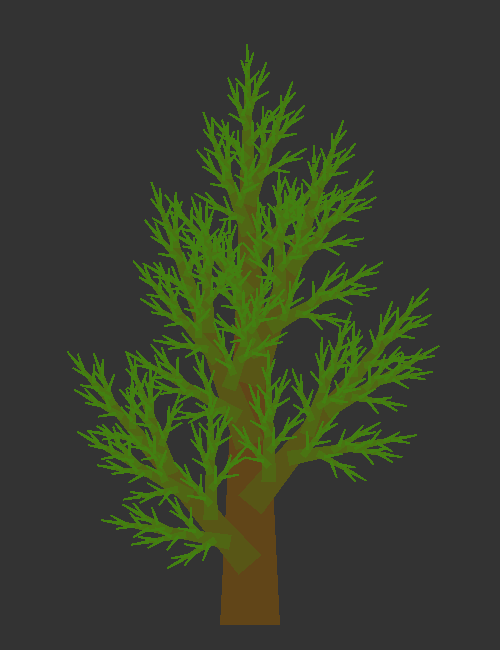
\includegraphics{res/gloss/gloss-tree.png}
	\vspace{1em}
	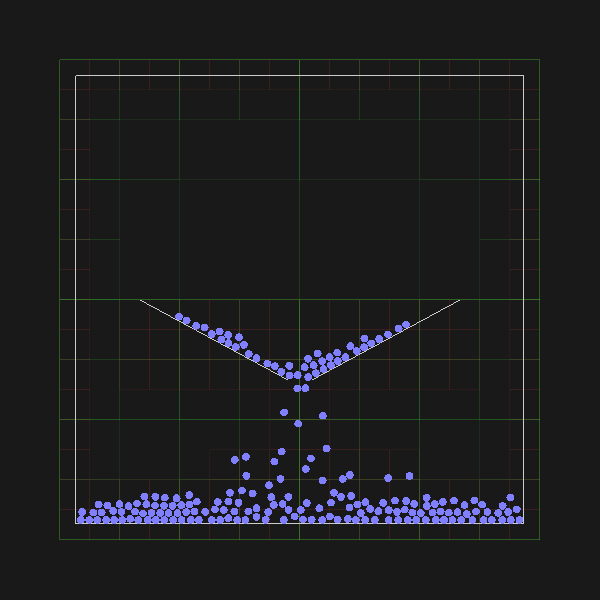
\includegraphics{res/gloss/gloss-styrene.png}
	\caption[Gloss example screens.]{Gloss example screens from \url{gloss.ouroborus.net/}.}
	\label{fig:gloss}
\end{marginfigure}

Any game is clearly going to involve graphics in some capacity or another, but graphics are not something that at first sight seem suited to a functional language. There are, however, various graphical frameworks and bindings available for Haskell.

For the purposes of the Serenity project, the choice basically boiled down to three options. Firstly, there are bindings directly to OpenGL available; which would provide the most flexibility but also likely the most development time. Secondly there are the bindings to the SDL engine, along with all the various tools provided with its framework. Many of the existing games written in Haskell use SDL. Lastly there is the use of the simple but effective layer over GLUT and OpenGL provided by the Gloss library.

This was not an easy decision, and some time went into making it. The direction taken in the Serenity project was to use the Gloss library, mostly because of its simple interface and ease of use, given the limited time and large scope of the rest of the project. The advantages of Gloss can be appreciated by considering the two screens in Figure \ref{fig:gloss}. Both of these examples involve relatively simple code, which is almost entirely pure.

The decision to use Gloss has largely been held up, but there has been some problems due to features it lacks, the most notable being clipping. In the future it would probably be beneficial to replace Gloss with an in house framework providing a layer between the pure graphics code and impure bindings to OpenGL.

Some details of the OpenGL and Gloss approaches are given below to illustrate the differences and tradeoffs involved.

\subsection{Using OpenGL Directly}

\marginnote{{\bf NB} --- The OpenGL code in this section is based on the tutorial at \url{haskell.org/haskellwiki/OpenGLTutorial1} (retrieved April 2013).}
Writing OpenGL code in Haskell is in many ways similar to writing it in C++ or any similar language. OpenGL calls are simply functions in the IO monad, (i.e. functions of type "IO a"), and there are some special primitive types such as "GLFloat". 

Listing~\ref{list:openglbasic} shows a very simple example of drawing an empty circle and a filled circle, and the output is shown in Figure~\ref{fig:openglbasicout}. Normal Haskell style is used to create a circle: using the "map" function and some trigonometry. These are then converted into OpenGL actions and rendered in the display callback. 

\vspace{-0.5em}
\begin{listing}{list:openglbasic}{Simple OpenGL example, drawing an empty circle and a filled circle (output shown in Figure~\ref{fig:openglbasicout}).}{Simple OpenGL example, drawing an empty circle and a filled circle (output shown in Figure~\ref{fig:openglbasicout}).}{}
\end{listing}\vspace{-1.5em}

\functions(myPoints, pointToVertex, renderMyPoints, display, main, flush, displayPrimitive, displayCallback, getArgsAndInitialize, mapM_, createWindow, mainLoop, clear, renderPrimitive)
\begin{haskell}

>import Graphics.Rendering.OpenGL
>import Graphics.UI.GLUT

>myPoints :: GLfloat -> [(GLfloat,GLfloat,GLfloat)]
>myPoints r = map (\k -> (r*sin(2*pi*k/n),r*cos(2*pi*k/n),0.0)) [1..n] 
>  where n = 100

>pointToVertex :: VertexComponent a => (a, a, a) -> IO ()
>pointToVertex (x,y,z) = vertex $ Vertex3 x y z

>renderMyPoints :: GLfloat -> IO ()
>renderMyPoints r = mapM_ pointToVertex (myPoints r)

>main = do 
>  (progname, _) <- getArgsAndInitialize
>  createWindow "OpenGL Example"
>  displayCallback $= display
>  mainLoop

>display = do 
>  clear [ColorBuffer]
>  renderPrimitive LineLoop (renderMyPoints 1)
>  renderPrimitive TriangleFan (renderMyPoints 0.5)
>  flush

\end{haskell}
\begin{marginfigure}[-25em]
	\hspace{-2em}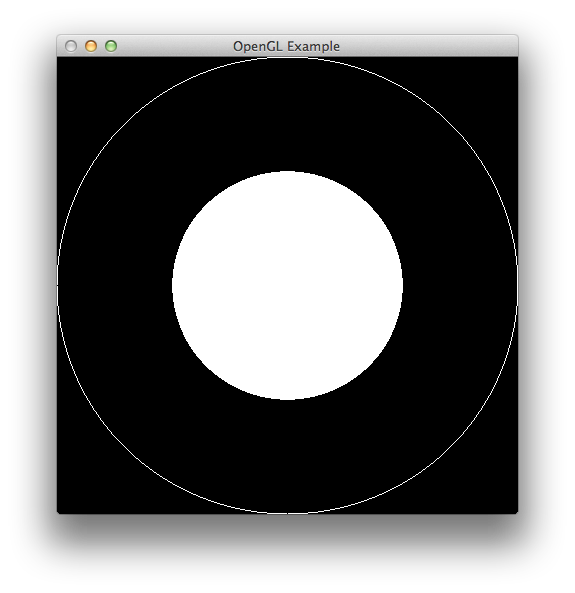
\includegraphics[width=18em]{res/opengl/openglbasic.png}
	\caption[Output of example OpenGL code in Listing~\ref{list:openglbasic}.]{Output of example OpenGL code in Listing~\ref{list:openglbasic}.}
	\label{fig:openglbasicout}
\end{marginfigure}
\vspace{-1em}
\noindent 
The challenge of programming graphics this way is far less an issue of language paradigm than it is of coding style: maintaining a proper separation between the concerns of basic rendering, specific entity models, the game logic, and so on, is the where main engineering effort is required --- and this is no different in Haskell than in other languages. 

As discussed in the previous section, there are various ways that such separation can be achieved, and that primary among these is the concept of an interim type. It is exactly this approach that is taken by the Gloss library, and this is the main reason Gloss was used in Project Serenity, to avoid the additional time it would take to build the infrastructure to work effectively with OpenGL.

\subsection{Using Gloss}

\begin{marginfigure}
	\hspace{-3em}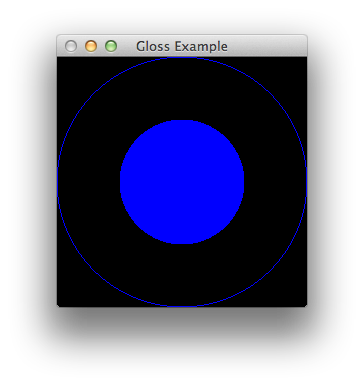
\includegraphics[width=21em]{res/gloss/glossbasic.png}
	\caption[Output of example Gloss code in Listing~\ref{list:glossbasic}]{Output of example Gloss code in Listing~\ref{list:glossbasic}.}
	\label{fig:glossbasicout}
\end{marginfigure}

Gloss is a layer that sits on top of OpenGL and GLUT providing a much simpler and cleaner API for drawing vector graphics. The Gloss project website claims that ``Gloss hides the pain of drawing simple vector graphics behind a nice data type and a few display functions'', and that using Gloss allows you to ``get something cool on the screen in under 10 minutes''.\sidenote[][1em]{See \url{hackage.haskell.org/package/gloss}} The simplicity of using Gloss compared to raw OpenGL code is shown in Listing~\ref{list:glossbasic} which recreates the simple OpenGL example in Gloss (although the colour of the circles has been changed to make the difference in outputs obvious).

\vspace{-0.5em}
\begin{listing}{list:glossbasic}{Example of simple Gloss usage}{Simple Gloss example, drawing an empty circle and a filled circle (output shown in Figure~\ref{fig:glossbasicout}).}{}
\end{listing}\vspace{-1.5em}

\functions(display, black, circles, color, blue, circleSolid, circle, play, playIO)
\begin{haskell}
>import Graphics.Gloss
>
>main = display (InWindow "Gloss Example" (250, 250) (0, 0)) black circles
>
>circles = Pictures $ map (color blue) [circleSolid 125, circle 250]

\end{haskell}
\noindent
This example simply creates a window named ``Gloss Example'' with a black background and adds the specified "Picture" to it. A "Picture" is the Gloss abstraction of the OpenGL primitives. In the example the picture to display is defined by the "circles" function.

The example in Listing~\ref{list:glossbasic} uses the "display" mode to draw a static picture to the screen. The game mode, started with "play" or "playIO", is obviously more useful when developing a game. It keeps track of a game world, the current state of the game, for which the developer provides callbacks for updating the world every tick and for converting the world to a "Picture". It also allows the programmer to add callbacks for handling input events such as mouse movement and clicks. The Gloss documentation and \texttt{gloss-examples} package are great sources of further information on getting started with game development with Gloss.\sidenote[][-5em]{See \url{hackage.haskell.org/package/gloss} and \url{hackage.haskell.org/package/gloss-examples}}

\subsection{Summary of this section} 
Given the limited time available for the Serenity project, the prebuilt pure interface onto OpenGL provided by the Gloss library was the best option, and this has been born out by the results. A custom made layer that is more appropriate for the needs of a complex game, and more readily adapted to changing requirements, would be beneficial to develop in the future.
\cleardoublepage
\section{Architectural Design --- Code Organisation and  Separation of Concerns}
\label{sec:architecture}

% Server vs lock step game design
% Shared parts of implementation between client and server 
% Layout of project
% IO and pure separation

When coming from an OO background, one of the first problems encountered when embarking on a large FP project is how to organise and architect the code. There is a certain paucity of literature pertaining to this issue; and while there are many projects on Hackage that provide good examples, the principles behind them are not always clear.\sidenote{CF Section \ref{sec:fp_review} on page \pageref{cf:code_organisation}. }

There are two related issues here. First is simply what files should have what code in them; and second, how to separate concerns effectively. These can be seen as quite separate issues, but it is helpful to consider them simultaneously here, as should become apparent.

Common practice in OO languages is to have one class per file\sidenote{See \url{www.oracle.com/technetwork/java/codeconv-138413.html} (rev. 1999) and \url{www.possibility.com/Cpp/CppCodingStandard.html\#cflayout} for example. (Accessed April 2013).} but it is not immediately clear what principle in FP should determine the contents of a file. The approach taken in the Serenity project is instead to allow \emph{form} to follow \emph{function} (no pun intended); that is, to allow the desired separation of concerns to drive the module layout --- adjusting as becomes necessary --- rather than a specific type of code concept.

The main separation of concern that every Haskell project is going to contain to some degree or another is between pure and impure code, and so the first thing to be considered in designing an architecture for a project should be how the connection and communication between these areas is going to be managed.
At first sight it would appear that almost all of what happens in a game is IO of some sort or another, but this is not the case. Code can be pure precisely when its output can be defined in terms of its arguments \emph{only}.\sidenote{CITATION NEEDED} Motion of a particle in space experiencing a force due to gravity, for example, can be defined in terms of pure code. The process of writing log entries into a file will not be, (although the code that designated the actual content of the entries could be).

This is all very well, but does not make it immediately clear how to break down a project's code. The approach taken during the design of Serenity's module structure, and the approach recommended by this guide, is to let the structure of the main loop of each runnable component guide the nature and interface of each module.

To demonstrate how this works, consider the architecture of the Serenity project. As discussed elsewhere,\sidenote{Section \ref{sec:specv2} page \pageref{sec:specv2}.} the game uses a server-client model, but with none or very limited simulation clientside. There are therefore two runnable components, which will share some logic. Each main loop will therefore have two main impure parts: the receiving of IO over the network from the server or client, and local IO (be it output to the screen, logging, or input from the user).

It is clear that some data structure must exist that models the state of the game. Because no simulation takes place on the client, all the updates to this structure will be due to messages from the server. User interactions also need to generate messages \emph{to} the server. So the client loop will consist of reading input from the network and updating the game state, rendering the screen, then reading input from the user and sending output to the network.

\begin{marginfigure}
	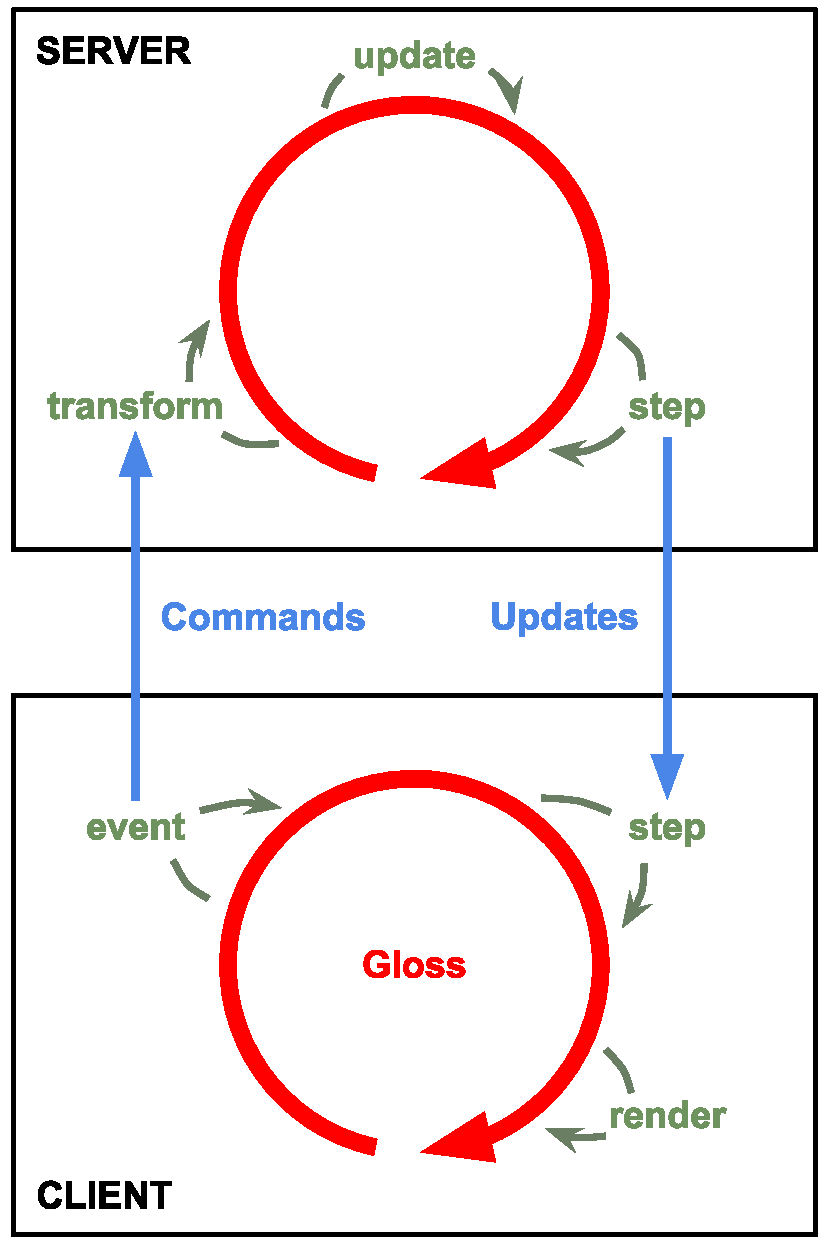
\includegraphics{res/architecture.pdf}
	\caption[Depiction of server and client main loops.]{Depiction of server and client main loops. The main loops are in red, the network exchanges in blue, and pure function calls in green.}
	\label{fig:loops}
\end{marginfigure}

Conversely the server loop must read input from the clients and store it, simulate the game world and send the result of this simulation to all clients. Figure \ref{fig:loops} is a diagram of the interaction between these two loops.

From this simple analysis of the required basic functionality, several concepts have already been defined. On top of the loops themselves, there is:

\begin{itemize}\itemsep-3pt
    \item the network exchange (which comes in two flavours, client to server and server to client) 
    \item the game state itself
    \item the rules for updating the game state in reaction to updates from the server
    \item the rules for updating the game state in reaction to time passing (i.e.\ the simulation)
    \item The rules for rendering the screen
\end{itemize}

\begin{marginfigure}[6em]
	\begin{itemize}\parskip-3pt
    \item Game \begin{itemize}\itemsep-3pt
            \item Server
            \item Client
        \end{itemize}
    \item Model\begin{itemize}\itemsep-3pt
            \item Game state
            \item Time
        \end{itemize}
    \item Network
\end{itemize}
	\caption[The top level names in the module hierarchy in early versions of Serenity.]{The top level names in the module hierarchy in early versions of Serenity.}
	\label{fig:loops}
\end{marginfigure}

\noindent It should be clear that this has immediately imparted a basic way of breaking up the project, and if we examine the top level module namespaces in the early versions of the Serenity source it can be seen that they correspond largely with the above list (the main difference being that the graphics code was contained within the Client modules). But it has also provided a guide to the IO/pure separation. The various parts of the game state, and the different ways in which it can be update (collectively referred to in the source as the \emph{model}) can be entirely pure. The network layer will clearly be impure, and can communicate representations of various aspects of the (pure) model.\sidenote{Bear in mind each of these headings does not need to --- and probably shouldn't --- represent one Haskell file. Instead they each represent  a top level module (rather like a package in Java) that is imported as one module but can be made up of several smaller internal modules.}

Surprisingly, the graphics logic is also entirely pure. This is because the code only has to define `what' to draw, in terms of an abstract "Picture" type. In the case of Serenity the actual impure drawing took place within the external library Gloss, but in projects where OpenGL (or similar) is used directly, it would still be wise to maintain this separation between a pure logic layer, and an impure `work' layer. This is an important and widely used concept, and is the subject of Section \ref{sec:pure}.

\paragraph{Summary of this section} Two important patterns have emerged during this discussion. Firstly there is the approach to setting out the top level breakdown of a large project: by considering units of functionality from the point of view of the main loop of the program and how these parts interface. This leads to both a decent module breakdown and a insight into the appropriate separation of pure and impure code.
\cleardoublepage
\section{Haskell Modules, Encapsulation, and Connascence}
\label{sec:encapsulation}

Connected with separation of code and concerns are the subjects of \emph{encapsulation} and \emph{Connascence}. Encapsulation (sometimes referred to as \emph{information hiding}) is the maintenance of a public interface that allows for implementation changes to be made without breaking another component that imports it, whereas connascence is a more general term for when modifying one piece of code must lead to modifying another in order to maintain correctness. Two pieces of code are connascent when a change in one necessitates a change in the other.\citefix{page1992comparing}

Compared with Java and other similar OO languages, more effort has to be made in Haskell to have good encapsulation between modules. No formal effort was made to address encapsulation issues at the beginning of the Serenity project, and this has led to some (small) problems in a few places. In response to these, the conventions discussed below were adopted.

Most of the issues with encapsulation in Haskell are due to user defined types using the "data" keyword. Exporting constructors directly is bad encapsulation, because changes to the structure of the type can lead to dependant implementations failing. For example consider the simple datatype in a module shown in Listing \ref{list:encapsulation_bad}.

\vspace{-0.5em}
\begin{listing}{list:encapsulation_bad}{An example of a badly encapsulated module interface.}{An example of a badly encapsulated module interface.}{}
\end{listing}\vspace{-1.5em}

\begin{haskell}
>module MyApp.Test where

>data Example = Example Int Int

\end{haskell}
\noindent
This leads to strong connascence between this module and any other importing it, because if an additional field were to be added to the "Example" type, every other module using the "Example" constructor would no longer compile. It also exposes the internals of the type and is such is bad encapsulation --- another module could come to rely on the way information is represented in the type and then break when changes to the implementation are made.

The way to manage this is to use the Haskell record syntax, and to only export the field functions, and an abstract constructor (or constructors). This approach is shown in Listing \ref{list:encapsulation_good} below.

\vspace{-0.5em}
\begin{listing}{list:encapsulation_good}{A well encapsulated module interface.}{A well encapsulated module interface.}{}
\end{listing}\vspace{-1.5em}

\begin{haskell}
>module MyApp.Test (example, exampleOne, exampleTwo) where

>data Example = Example { exampleOne :: Int, exampleTwo :: Int }

>example :: Int -> Int -> Example
>example = Example

\end{haskell}
\noindent
Now the exported functions --- "example", "exampleOne", "exampleTwo" --- are the only available public interface to the module. If a field is added, or the internals of the type representation change, these three functions can be maintained (even if they are no longer defined through the record syntax). The implementation details of the module are now hidden and other modules importing it do not become connascent to it.

There are various further improvements to this. Exporting lenses, rather than the basic deconstruction functions provided by the record syntax, is desirable.\sidenote{Lenses are the functional equivalent of setters and getters and key value coding. See Section \ref{sec:gui} below.} Also there are language extensions such as GADTs (Generalised Algebraic Datatypes) that can take this kind of method further.\sidenote[][3em]{For more information on GADTs see \url{http://en.wikibooks.org/wiki/Haskell/GADT} (accessed April 2013) or \bibentry{pottier2006stratified}.}

Another desirable feature is to have a single point of entry for other modules to import a set of functionality. For this reason it is a desirable pattern to have a single module "App.X" for example, that re-exports the public interface of every module underneath it ("App.X.One", "App.X.Two" etc). Another module "App.Y" should only import "App.X" and not the inner parts of its implementation. This way module "App.X" can take care of the overall public interface, whereas modules underneath it in the hierarchy can share some implementation details if needed.

As well as providing encapsulation and avoiding connascence, this pattern leads to cleanly separated interfaces and can avoid problems with circular imports. 

\paragraph{Summary of this section} Some more care must be taken with encapsulation in Haskell than in OO languages like Java. However, it can be achieved by sticking to a couple of simple rules: don't export constructors directly, and keep inner module implementations cleanly separated.
\cleardoublepage
\section[On the Separation of Interface from Implementation and Cause from Effect]{On the Separation of Interface from Implementation and Cause from Effect}
\label{sec:pure}

There has already been some discussion about separating pure code and code that must interact with the outside world in Section~\ref{sec:architecture}, and on reducing dependency between components in Section~\ref{sec:encapsulation}. Here we discuss more specific design patterns that can address these and similar issues, in the more general setting of separation between interface and implementation.

\subsection{Classes}

Of primary importance in Haskell coding is the concept of \emph{classes}, distinct from classes in an OO context. In Haskell, a type is an instance of a class if a given set of functions are provided. For example, Listing \ref{list:functor} shows the class declaration for a \emph{functor}.

\vspace{-0.5em}
\begin{listing}{list:functor}{The \emph{Functor} typeclass}{The \scalenote{"Functor"} typeclass.}{}
\end{listing}\vspace{-1.5em}

\begin{haskell}
>class Functor f where
>  fmap :: (a -> b) -> f a -> f b

\end{haskell}
\noindent Here, "f", "a", and "b" are type variables; "f" representing the type belonging to the class, and "a" and "b" able to be any types. For example, if the type "f" was "[]" (i.e.\ the list type) then it is easy to see that "fmap" is the same type as the normal "map", and a therefore possible "Functor" instance (which is actually already the default instance) for a list is as shown in Listing~\ref{list:listfmap}.

\vspace{-0.5em}
\begin{listing}{list:listfmap}{A \emph{Functor} instance for lists}{A \scalenote{"Functor"} instance for lists.}{}
\end{listing}\vspace{-1.5em}

\begin{haskell}
>instance Functor [] where
>  fmap = map

\end{haskell}
\noindent The advantage that this gives is that it is now possible to write functions that know nothing about the type of their inputs other than that they are an instance of some class. For example, we could define a version of "fmap" that works on a pair of different functors, like so:

\vspace{-0.5em}
\begin{listing}{list:pairfmap}{Example of writing a function using only the knowledge that the argument is a Functor}{Example of writing a function using only the knowledge that the argument is a \scalenote{"Functor"}.}{}
\end{listing}\vspace{-1.5em}

\begin{haskell}
>fmap2 :: (Functor f1, Functor f2) => 
>  (a -> b) -> (c -> d) -> (f1 a, f2 c) -> (f1 b, f2 d)
>fmap2 g1 g2 (x,y) = (fmap g1 x, fmap g2 y)

\end{haskell}
\noindent This function can now be used whenever "Functor" instances are available on both types in a pair. This is a contrived example, but hopefully illustrative of the advantages of this approach --- designing a module so that it works on any instance of a given class, be it an inbuilt one like "Functor", or a new class provided by the module, is an excellent way to avoid coupling and allow for code reuse.

This pattern is used in several places in the Serenity code, most notably to provide a clean interface between the implementation of the model and the code that updates state during the game. Listing \ref{list:timeclasses} shows an extract from "Serenity.Model.Time" showing the classes used to provide this interface. There are three classes, "Updatable", "Commandable", and "Evolvable", to represent to concepts of reacting to updates from the server, commands received from the client, and to the passing of time. Class inheritance (similar to inheritance in OO) is used so that an instance of "Commandable" or "Evolvable" must already be an instance of "Updateable".

\vspace{-0.5em}
\begin{listing}{list:timeclasses}{Classes from \emph{Serenity.Model.Time}}{Classes from \scalenote{"Serenity.Model.Time"}.}{}
\end{listing}\vspace{-1.5em}

\functions(update, updates, command, commands, evolve, pure)
\begin{haskell}

>class Updateable a where
>  update  ::  Update  -> a -> a
>  updates :: [Update] -> a -> a
>  updates = flip (foldr update)

>class (Updateable a) => Commandable a where
>  command  ::  Command  -> a -> [Update] 
>  commands :: [Command] -> a -> [Update]
>  command _ _ = []
>  commands cs a = concatMap (flip command a) cs

>class (Updateable a) => Evolvable a where
>  evolve :: UpdateWire (a, Game)

\marginnote[-1em]{\anote The type \scalenote{"UpdateWire"} is an object that gives logic for providing updates given the passing of time.}\vspace{-1.7em}
>  evolve = pure []

\end{haskell}
\noindent After this, all the server and client logic uses only these interfaces. This means that any types providing instances for these classes could take advantage of the server-client code --- this could be a completely different game! The proper usage of classes allows for a great deal of reusability. 

\subsection{Separating Syntax and Semantics Part I: Interim Types}

A very fundamental design pattern is to distinguish as much as possible between the form of a representation and its semantics. A classic example of this is the organisation of compilers into a front and back end. The front end is responsible for building a representation of the input string, usually in the form of an abstract syntax tree (AST), and the back end is responsible for converting the AST into code for the target system. This modularity confers a number of advantages, the foremost being that $n$ input languages and $m$ target architectures require only $n+m$ implementations rather than $nm$.\citepage{grune2012modern}{page 6, section 1.1.1.}

This technique can be found throughout the Haskell runtime and in many of the popular Haskell libraries. The IO monad that allows a running Haskell program to interact with the real world is a perfect example. During compilation, actions in the IO monad are simply descriptions of operations to be performed, that can only be semantically interpreted to yield actual values at runtime.\cite{peyton1993imperative}

A motivating example will help to demonstrate the efficacy and need for this design pattern. Consider an entity within the state of a game. At various points this entity will need to be updated in various ways to react to different things. For the purposes of the running example we shall model: time passing, new orders being given from the player, and damage being inflicted. (This is clearly in the context of a strategy game similar to that made in the Serenity project).

First some basic types are defined, without specific implementation details for brevity, for an entity, a command, and an amount of damage.

\vspace{-0.5em}
\begin{listing}{list:entitytype}{Some basic types for the entity update example}{Some basic types for the entity update example.}{}
\end{listing}\vspace{-1.5em}

\functions()
\begin{haskell}

>data Entity = Entity {...}
>data Order = Order {...}
>data Damage = Damage {...}

\end{haskell}
\noindent Now the three types of update are to be implemented. Although these updates must eventually be applied ``in the real world'' by an IO routine, their behaviour can still be defined by pure functions. So an initial implementation might look like this:

\vspace{-0.5em}
\begin{listing}{list:basicentity}{A naive approach to entity semantics}{A naive approach to entity semantics.}{}
\end{listing}\vspace{-1.5em}

\functions(updateTime, updateOrder, updateDamage)
\begin{haskell}

>updateTime :: Double -> Entity -> Entity
>updateTime time entity = ...

>updateOrder :: Order -> Entity -> Entity
>updateOrder order entity = ... 

>updateDamage :: Damage -> Entity -> Entity
>updateDamage damage entity = ...

\end{haskell}
\noindent With these three functions implemented, a basic interface for updating an entity can be exported. But it is not very flexible. To see why, consider the code applying the updates to the game state. The updates can be applied as they come in, or buffered in some structure, which for simplicity can be assumed to be a list. What type is the list? Without any further structure it can only be of type "[Entity -> Entity]" and each element is one of the update functions partially applied, i.e. "[updateTime 4.3, updateDamage Damage {...}, ...]". Now say the writer of this code wants to add some additional behaviour as the "Entity" gets updated, such as logging, or notifying some other part of the state. He can't, as there is no way to introspect what is contained in each update, so any changes must be made to the update functions themselves, including their type signatures.

The solution is to use an interim type to separate the two concerns. This type will stand for the concept of \emph{some kind of update that could be applied to an Entity}.

\vspace{-0.5em}
\begin{listing}{list:entitymessage}{Entity update interim type}{Entity update interim type.}{}
\end{listing}\vspace{-1.5em}

\begin{haskell}

>data EntityUpdate = 
>  | UpdateTime Double
>  | UpdateOrder Order
>  | UpdateDamage Damage

\end{haskell}
\noindent This type provides a separation between the \emph{form} of, and the actual \emph{semantics} of, updating an entity. An instance of the type can be introspected (either via pattern matching or a proper provided interface --- the latter isn't detailed here to keep it simple), and other code is free to interpret the type in any way without making changes to it.

A semantics can of course be provided alongside this type as a simple function without removing the benefits gained by the separation. Listing \ref{list:entitydefaultsemantics} illustrates such a function. An implementation can now introspect and store updates, call this function, and add any additional behaviour required.

\vspace{-0.5em}
\begin{listing}{list:entitydefaultsemantics}{Providing a default semantics}{Providing a default semantics.}{}
\end{listing}\vspace{-1.5em}

\begin{haskell}

>update :: EntityUpdate -> Entity -> Entity
>update (UpdateTime t) = ...
>update (UpdateOrder o) = ...
>update (UpdateDamage d) = ...

\end{haskell}
\noindent This example illustrates a somewhat trivial case, but the general pattern is extremely advantageous, especially when it is not obvious how to limit the use of impure code. For example, this implementation could be extended by adding an IO routine to be called on each update, without needing to change the existing pure functions. 
The "Picture" type from the Gloss graphics library is an excellent example of this pattern in a real application. Instead of insisting that the caller uses IO drawing routines directly, the "Picture" type forms a pure interface to describe what \emph{should} be drawn.

\subsection[Modelling Effects with Monads and Monad Transformers]{Modelling Effects with Monads and Monad \\Transformers}

In the discussion thus far the state of the game or program has not been considered in detail. At first sight one might assume that impure code must be responsible, at least at some level, for the update of this state, but this is not actually the case. It is possible to pass state entirely functionally, as the following small example of a stack machine demonstrates:

\vspace{-0.5em}
\begin{listing}{list:basicstack}{Modelling a simple stack machine using pure code only}{Modelling a simple stack machine using pure code only.}{}
\end{listing}\vspace{-1.5em}

\functions(eval, run)
\begin{haskell}

>data Operation a = Push a |Pop |Sum |Diff |Mult |Dup

>data State a = State {stack :: [a]}

>eval :: Num a => Operation a -> State a -> State a
>eval (Push a) (State s) = State (a:s)
>eval Pop  (State s) = State (tail s)
>eval Sum  (State (a:b:s)) = State (a+b:s)
>eval Diff (State (a:b:s)) = State (a-b:s)
>eval Mult (State (a:b:s)) = State (a*b:s)
>eval Dup  (State (a:s)) = State (a:a:s)

>run :: Num a => [Operation a] -> State a -> State a
>run = flip $ foldl $ flip eval

\end{haskell}
\noindent But this approach has a number of weaknesses. Firstly, passing state has to be dealt with manually, both in the type signatures and in the implementations, and there is the difficulty of extending the implementation to deal with errors or other concerns.

An effective pattern for modelling objects that have this kind of imperative structure is to use a \emph{monad},\citefix[-5em]{wadler1992essence} and indeed monads have become quite ubiquitous in Haskell programming despite having a somewhat ill-founded reputation for being hard to understand.\citefix{peyton2001tackling}

Existing familiarity with monads will not be assumed here, but the details are covered only very briefly.\sidenote{There are numerous online resources containing explanations of monads. \bibentry{lipovavca2011learn} contains an excellent introduction, and can be read online at \url{learnyouahaskell.com/}.} Listing \ref{list:effectmonad} shows the "Monad" typeclass.

A monad "m" can be thought of as a computational environment, where objects or routines can be combined using ">>=" (pronounced `bind') and "return" provides a way `into' the context. Notably here, the implementation of ">>=" can thread a state through a sequence of computations, and cause this state to be updated in any number of ways at each stage, reacting to errors etc. For this reason a monadic value "m a" is sometimes referred to as a monadic \emph{action}.

\vspace{-0.5em}
\begin{listing}{list:effectmonad}{The \emph{Monad} typeclass}{The \scalenote{"Monad"} typeclass.}{}
\end{listing}\vspace{-1.5em}

\functions(get, put, modify, runState, execState, evalState)
\begin{haskell}

>class Monad m where
>  return :: a -> m a
>  (>>=) :: m a -> (a -> m b) -> m b

\end{haskell}
\noindent 
The standard Haskell distribution comes with a number of monads built in, including the "State" monad, which provides an environment that keeps track of a generic state. Inbuilt functions "get", "put", and "modify" are provided to put values into the state, get them out, and call a function over the contents of the state respectively. Listing \ref{list:statestack} shows the state machine example re-written to use the "State" monad.

\vspace{-0.5em}
\begin{listing}{list:statestack}{Modelling a simple stack machine using pure code with the \emph{State} monad}{Modelling a simple stack machine using pure code only, this time using the \scalenote{"State"} monad.}{}
\end{listing}\vspace{-1.5em}

\functions(popM, pushM)
\begin{haskell}

>import Control.Monad.State

>type StackMachine a = State [a]

>popM :: StackMachine a a
>popM = do
>  (x:xs) <- get
>  put xs
>  return x

>pushM :: a -> StackMachine a ()
>pushM x = do
>  stack <- get
>  put (x:stack)

>eval' :: Num a => Operation a -> StackMachine a ()
>eval' (Push a) = pushM a
>eval' Pop  = do popM; return ()
>eval' Sum  = do a <- popM; b <- popM; pushM (a+b)
>eval' Diff = do a <- popM; b <- popM; pushM (a-b)
>eval' Mult = do a <- popM; b <- popM; pushM (a*b)
>eval' Dup  = do a <- popM; pushM a; pushM a

>run' :: Num a => [Operation a] -> StackMachine a ()
>run' = foldM (\_ -> eval') ()

\end{haskell}
\noindent The function "execState" can be used to find the value of the state after a computation, so the expression

\begin{haskell}

>execState (run' [Push 10, Push 5, Mult]) []

\end{haskell}
\noindent will yield "[50]".

Note that no state is passed manually, and the implementation of "eval'" is dependent only on the interface to the monad "StackMachine a". From now on, extra functionality can be added by changing the implementation of the monad, without effecting the implementation of "eval'". 

To further illustrate this point, consider the following. Currently this implementation will crash if operations are made when the stack does not have the required number of elements:

\begin{verbatim}
> execState (run' [Push 10, Mult]) []
*** Exception: Pattern match failure in do expression
\end{verbatim}

\noindent To improve this, an error mechanism can be added to the monad by using a \emph{monad transformer}. A monad transformer is a monad formed by `wrapping' an existing monad, so that "return" and "(>>=)" perform both the original monad's implementation and some additional functionality provided by the transformer. Monadic actions can be performed on the inner monad by using a lifting function. All that needs to be changed is the type synonym "StackMachine" to wrap a "Maybe" value\sidenote[][-8em]{\scalenote{"Maybe"} is used here, which models the computation either succeeding with a value or failing, but does no error reporting. However, if error reporting is required, the \scalenote{"Either"} monad or the \scalenote{"Error"} monad can be used.} in a state monad transformer (using the "StateT" constructor), and the implementation of "popM", as shown in Listing~\ref{list:statestackerror} below.

\vspace{-0.5em}
\begin{listing}{list:statestackerror}{Adding error handling using \emph{Maybe} and the state monad transformer}{Adding error handling using \scalenote{"Maybe"} and the state monad transformer.}{}
\end{listing}\vspace{-1.5em}

\functions(lift)
\begin{haskell}

>type StackMachine a = StateT [a] Maybe

>import Control.Monad.State

>popM :: StackMachine a a
>popM = do
>  stack <- get
>  case stack of
>    (x:xs) -> do put xs; return x
>    _ -> lift Nothing

\marginnote[-1.5em]{\anote The \scalenote{"lift"} function is used to access the inner monad, here causing the computation to fail by passing \scalenote{"Nothing"} into the \scalenote{"Maybe"} monad.}

\end{haskell}
\noindent Without any further changes, the following results are obtained:

\begin{verbatim}
> execStateT (run' [pushM 10, pushM 5, Mult]) []
Just [50]
> execStateT (run' [pushM 10, Mult]) []
Nothing
\end{verbatim}

\noindent Extending this to include error reporting or different modes of failure is achievable just as easily.

It should be apparent that modelling effects using monads provides a good number of advantages, from separation of concerns to elegance of code. Writing new monads can be tricky, but the desired effects can usually be easily achieved by combining existing monad transformers. It is these advantages that make the monad such a widely used design pattern in Haskell code.

\subsection{Separating Syntax and Semantics Part II: Free Monads}
\label{ssec:freemonads}

\functions(liftF, retract, hoistFree)
A further technique for improving the separation between interface and implementation is the usage of \emph{free monads}, a relatively recent research area in the Haskell community.\sidenote{In the examples below, the free monad implementations come from Edward Kemmet's package \emph{free} (\url{hackage.haskell.org/package/free}), which also provides the functions \scalenote{"liftF"}, \scalenote{"retract"}, and \scalenote{"hoistFree"}. Various other free monad implementations are also available on Hackage.} 
The use of free monads as a design pattern was only discovered and experimented with after the main bulk of Project Serenity was already implemented, and there are many parts of the design that could benefit a great deal by being refactored to make use of it. The use of free monads and why they can be so useful is the subject of the rest of this section.

The precise definition of a \emph{free} structure is a concept from Category Theory and out of the scope of any discussion here; but like monads, the technical details are not required to make use of the pattern as a programmer.

In simple terms, then, a free monad is a monad that can be generated directly from a functor ``for free'' --- i.e. without any additional information being given or imposed. This is achieved by maintaining the structure of the operations (as a list or stream) without actually interpreting them. A monadic value in this free monad can then be interpreted, i.e. converted to a monadic value in another monad by imposing a certain semantics, at any time at a later date, and even in multiple ways at different times.

Consider the stack machine example. After "run" (or "run'") has been called, the computation is complete and the components of it cannot be introspected in any way. So, while there is a compile time separation provided between the "Operation" type and the "StackMachine" monad, at runtime a "StackMachine" monadic value is essentially opaque.

To improve upon this situation, a free monad can be formed from the "Operation" type. A wrapper is used to form a functor, with an additional type variable that represents ``the rest of the computation'' or continuation (the functor instance can be automatically derived). From this functor the free monad is formed. The code for this is shown below in Listing~\ref{list:freeoperation}.

\vspace{-0.5em}
\begin{listing}{list:freeoperation}{Forming a free monad from the \emph{Operation} type}{Forming a free monad from the \scalenote{"Operation"} type.}{}
\end{listing}\vspace{-1.5em}

\functions(liftFF, push, pop, sum, diff, mult, dup, example, interpret, using)
\begin{haskell}
>data FreeFunctor a cont = FreeFunctor a cont 
>  deriving (Functor, Show)

>type AbstractMachine a = Free (FreeFunctor (Operation a))

>liftFF :: a -> Free (FreeFunctor a) ()
>liftFF x = liftF $ FreeFunctor x ()

>push a = liftFF $ Push a
>pop = liftFF Pop
>sum = liftFF Summ
>diff = liftFF Diff
>mult = liftFF Mult
>dup = liftFF Dup

>example :: AbstractMachine Int ()
>example = do push 9; push 5; mult; dup; mult

>interpret :: (Functor m, Monad m) => (forall x. f x -> m x) -> Free f a -> m a
>interpret f = retract . hoistFree f

>using :: Monad m => (t -> m a) -> FreeFunctor t b -> m b
>using actionFor (FreeFunctor operation c) = do actionFor operation; return c

\end{haskell}
\noindent
The "interpret" function can now be used to coerce a value of type "AbstractMachine a" (the free monad) into a full monadic type with a specific semantics. "using" is a shortcut to lift a function between operations and actions into the type required by "interpret".

Three example semantics are shown in Listing~\ref{list:freesemantics}, firstly the normal operation of "StackMachine" with failure as implemented before, secondly some basic logging as a writer monad transformer, and lastly both of these simultaneously. 

\vspace{-0.5em}
\begin{listing}{list:freesemantics}{Three example semantics for the \emph{AbstractMachine} free monad}{Three example semantics for the \scalenote{"AbstractMachine"} free monad, the stack machine operation, basic logging, and both simultaneously.}{}
\end{listing}\vspace{-1.5em}

\functions(asStackMachine, asLog, asStackMachineWithLog, tell)
\begin{haskell}
>log :: (Show a, MonadWriter [Char] m) => Operation a -> m ()
>log (Push a) = tell $ "Pushing " ++ show a ++ "\n"
>log Pop  = tell "Popping"
>log Summ = tell "Summing\n"
>log Diff = tell "Subtracting\n"
>log Mult = tell "Multiplying\n"
>log Dup  = tell "Duplicating\n"

>asStackMachine :: Num a => FreeFunctor (Operation a) c -> StackMachine a c
>asStackMachine = using eval'

>asLog :: (Monad m, Show a) => FreeFunctor (Operation a) c -> WriterT String m c
>asLog = using log

>type StackMachineLog c = WriterT String (StackMachine a) c
>asStackMachineWithLog :: (Show a, Num a) => FreeFunctor (Operation a) c -> StackMachineLog c
>asStackMachineWithLog ff = do lift $ asStackMachine ff; asLog ff

\end{haskell}
\noindent
These results can now be obtained in GHCI:

\begin{verbatim}
> execStateT (interpret asStackMachine test) []
\end{verbatim}\vspace{-1em}
>Just [2025]

\begin{verbatim}
> putStr $ runIdentity $ execWriterT (interpret asLog test)
Pushing 9
Pushing 5
Multiplying
Duplicating
Multiplying

> fmap snd $ runStateT (runWriterT (interpret asStackMachineWithLog test)) []
\end{verbatim}\vspace{-1em}
>Just [2025]

\begin{verbatim}
> fmap (snd.fst) $ runStateT (runWriterT (interpret asStackMachineWithLog test)) []
\end{verbatim}\vspace{-1em}
>Just "Pushing 9\nPushing 5\nMultiplying\nDuplicating\nMultiplying\nPushing 9\nSubtracting\n"

\ 

\noindent
It is clear that this approach is a very effective and powerful one, and can be expanded to allow for easy combination of different layers of concern, each with their own semantic interpretation, loosely coupled and swappable. There are several packages that build on this idea and make working with it easy, the most notable being \emph{operational},\sidenote[][-2em]{Heinrich Apfelmus 2011, \url{hackage.haskell.org/package/operational}} a package for building custom monads, and \emph{pipes},\sidenote{Gabriel Gonzalez 2013 \url{hackage.haskell.org/package/pipes}} which models separate interpretation layers as a pipeline, allowing for filtering at each stage, and passing information in both directions. These kind of design patterns are invaluable to complex systems like games, that require multiple states to be maintained at the same time as networking, journalling, and various other activities; and their use is highly recommended in any similar domain.

\subsection{Summary of this section}

High level abstractions enabled by features of the Haskell language and type system can enable an extremely flexible coding style that maintains clear separation between concerns, and implementation from interface. The design patterns identified in this section give methods toward achieving these ends in a reliable way.

Typeclasses are a basic language feature of Haskell, and provide a simple yet highly effective was to write reusable code components. A very powerful idiom for flexible code is to use interim types to separate concerns. Monads provide a very flexible approach to modelling effects, and this can be improved even further with the use of free monads.

\cleardoublepage
\section{Networking}

% How the problems of game networking were solved in the network layer

Lorum ipsum sit dolor amet.\citefix{church1932}  \lipsum[2-4]\cleardoublepage
\section{Implementing a Graphical User Interface (GUI) Framework, and the Power of Lenses}
\label{sec:gui}

Gloss provided an interim layer to abstract away the complexities of OpenGL and impure drawing code, but as it turned out further abstractions on top of this were desirable. Gloss provides no ``widgets'' (buttons, scroll bars, etc), nor does it facilitate separable concerns for event handling.

Some time was spent in developing a framework on top of Gloss to enable easier construction of graphical interfaces, which has been glibly titled \emph{Sheen}\index{Sheen}. Provided by Sheen is a mechanism for event handling, recursively nested views, and various pre-built widgets such as labels, buttons, and text boxes. The best approach to the design of Sheen was not obvious, and its structure, and use of \emph{lenses} (see below) is considered to be quite novel and a demonstration of good Haskell style. This section considers various aspects of the Sheen design, but first it is worth examining lenses as significant use of them are made in the framework.

\subsection{On Lenses}

A lens is the functional equivalent of a setter and a getter at the same time. One way of thinking of a lens is it having the type

\functions(view, get, set, lens)
>data Lens a b = {get :: a -> b, set :: b -> a -> a}

Normally lenses are not actually implemented this way, but in such a way to be isomorphic to this. The most popular implementation of lenses is currently in the \emph{lens} package by Edward Kmett,\sidenote{Edward A. Kmett, Copyright 2012-2013 \url{https://github.com/ekmett/lens/}.} which uses a generalised form of a so called van Laarhoven lenses. A van Laarhoven lens as type

>type Lens a b = forall f. Functor f => (b -> f b) -> a -> f a

and the generalised notion of a lens family has type

>type LensFamily a b c d = forall f. Functor f => (c -> f d) -> a -> f b

The advantage of this definition of lenses is that they can be composed normally as functions using "(.)" and "id" from the Haskell prelude. This, and the large number of combinators provided in the \emph{lens} package, is what makes lenses so vastly useful. For a full technical explanation of this implementation of lenses see \url{comonad.com/reader/2012/mirrored-lenses}; here the way they are used is all that need be considered.

\functions(makeLenses, makeClassy, _bar, _baz, bar, baz, sndLens)
There are two ways of creating lenses. First is to use the "lens" function to build the lens from a getting and setting function directly, for example

>sndLens = lens snd (\(a,_) b -> (a,b))

This leads to a lot of boilerplate however. The alternative is to use the template Haskell routines provided in the library, "makeLenses" or "makeClassy". These do require Template Haskell (and hence GHC) but are very useful indeed. In the expression

>data Foo a = Foo
>  {  _bar :: a
>  ,  _baz :: [a]
>  }
>makeLenses ''Foo

the last line will create two addition functions

>bar :: Functor f => (a -> f a) -> Foo a -> f (Foo a)
>baz :: Functor f => ([a] -> f [a]) -> Foo a -> f (Foo a)

\cleardoublepage
\section{Modelling Time: Functional Reactive Programming}
\label{sec:frp}

\begin{itemize}
    \item Intro to FRP and how we used it
    \item Why it can be a bit problematic
\end{itemize}
\cleardoublepage
\section[Effective Unit Testing with Quickcheck and HUnit]{Effective Unit Testing with Quickcheck and \\HUnit}
\label{sec:testing}

% Find problems early
% Facilitates change

% \subsection{HUnit}

The HUnit library is the Haskell implementation of the standard xUnit unit testing framework. The
basic idea of the HUnit library is to provide the functions under test with some example data
and to compare the actual result with the expected result.

\vspace{-0.5em}
\begin{listing}{list:hunit}{Example usage of HUnit}{Example usage of HUnit. Testing a function that returns the length of a list.}{}
\end{listing}\vspace{-1.5em}

\functions(testEmpty, testTwo, tests, assertEqual, len)
\functions(runTestTT)
\begin{haskell}
>import Test.HUnit
>
>testEmpty = TestCase $ assertEqual "Empty list is zero" (len []) 0
>testTwo = TestCase $ assertEqual "List length two" (len [0, 1]) 2
>tests = TestList [testEmpty, testTwo]

\end{haskell}
\noindent An example of a small set of tests is shown in Listing~\ref{list:hunit}. This example shows
two simple tests for a function, "len", that returns the length of a given list.
A test, or list of tests, can be run with the use of the "runTestTT" function:

\begin{verbatim}
ghci> runTestTT tests
Cases: 2  Tried: 2  Errors: 0  Failures: 0
\end{verbatim}

% \subsection{QuickCheck}

\noindent Property based testing is a higher level approach to testing in which the programmer develops a specification
for the code to be testing. QuickCheck is a type-based property testing library that generates test
cases automatically from the developer defined expected properties.\cite{claessen2000} These properties
need to be true for all inputs to the function (i.e.\ invariants). This is an extremely
powerful approach to testing that allows the developer to write short testable specifications that
are used to verify the code with thousands of test cases which would be infeasible to write by hand.

\vspace{-0.5em}
\begin{listing}{list:quickcheck}{Example usage of QuickCheck}{Example usage of QuickCheck. Properties of a function that returns the absolute value of a number.}{}
\end{listing}\vspace{-1.5em}

\functions(prop_NonNegativity, prop_Multiplicativeness, prop_Subadditivity, prop_Idempotence, prop_Symmetry, absolute)
\functions(quickCheck, quickCheckWith, maxSuccess, verboseCheck)
\begin{haskell}
>import Test.QuickCheck
>
>prop_NonNegativity x = absolute x >= 0
>prop_Multiplicativeness x y = absolute (x * y) == (absolute x) * (absolute y)
>prop_Subadditivity x y = absolute (x + y) <= (absolute x) + (absolute y)
>prop_Idempotence x = absolute (absolute x) == absolute x
>prop_Symmetry x = absolute (-x) == absolute x

\end{haskell}
\noindent Listing~\ref{list:quickcheck} shows an example use case of QuickCheck to define five properties
of a function, "absolute", that returns the absolute value of a given number. The tests can then
be run by invoking the "quickCheck" function on one of the properties, for example:

\begin{verbatim}
ghci> quickCheck (prop_NonNegativity :: Integer -> Bool)
+++ OK, passed 100 tests.
\end{verbatim}

\noindent
This means that for one hundred randomly generated test cases the property held. It is
possible to get QuickCheck to run a different number of tests by using the "quickCheckWith"
function and specifying a different number for the "maxSuccess" argument. The actual
test cases that were generated can be viewed by using "verboseCheck" instead of "quickCheck"
--- be warned that, as the name implies, this is very noisy!

Testing is another area where the separation of pure and impure code becomes very useful.
By using the techniques laid out in the previous sections it is possible to have the majority
of game logic in pure functional code. This is of great benefit when it comes to testing
because, as Claessen and Hughes state, ``functional programs are well suited to automatic
testing''.\cite{claessen2000} Referentially transparent functions are much easier to test
than those that produce side-effects because program state before and after execution
is a nonissue.

During the development of the Serenity project an effective testing method combining the
use of QuickCheck and HUnit was found. QuickCheck was used to generate large numbers of
test cases for individual pure functions, and HUnit for impure functions, such as network
code, and units of code comprised of several functions used together. This approach allows
using the powerful property based testing where applicable in conjunction with more specific
HUnit test cases to maximise test coverage and confidence that the expected results are
being produced.

% Example from Serenity

\subsection{Organising an automated test suite}

When creating a test suite for your software project it is useful to organise it in such
a way as to allow quick automated testing, i.e.\ being able to run the entire test suite
with a single command. The easiest way to do this in a Haskell project is to use the
\texttt{test-framework} library. This library enables the user to group lists of tests
into cohesive units and then run a list of tests and test groups with a single function
call.

\vspace{-0.5em}
\begin{listing}{list:testframework}{Running tests with test-framework}{Running tests with test-framework}{}
\end{listing}\vspace{-1.5em}

\functions(main, defaultMain, allTests)
\begin{haskell}
>import Test.Framework
>
>main = defaultMain allTests
>
>allTests =
> [ Packet.tests
> , Transport.tests
> , Message.tests
> -- ...
> , MathUtil.tests
> ]

\end{haskell}
\noindent Listing~\ref{list:testframework} is an extract from the main entry point to
the Serenity test suite. It creates a list of tests from the test groups exported by
individual test modules. These tests are run by the "defaultMain" function provided by
"Test.Framework".

Grouping HUnit and QuickCheck tests with \texttt{test-framework} requires the use of
two further libraries, \texttt{test-framework-hunit} and \texttt{test-framework-quickcheck2}.
These two libraries provide functions to convert HUnit assertions and QuickCheck properties
into the "Test" type used by \texttt{test-framework}. A brief example of their use
in Serenity to build a group of tests to export is shown in Listing~\ref{list:testgroup}.

\vspace{-0.5em}
\begin{listing}{list:testgroup}{Grouping tests with test-framework}{Grouping tests with test-framework}{}
\end{listing}\vspace{-1.5em}

\functions(testGroup, testCase, testProperty, testReadNTChan, testReadTChanUntilEmpty, prop_EmptyTChan)
\begin{haskell}
>import Test.Framework (testGroup)
>import Test.Framework.HUnit (testCase)
>import Test.Framework.QuickCheck2 (testProperty)
>
>tests = testGroup "Network utility tests"
> [ testCase "Test readNTChan" testReadNTChan
> , testCase "Test readTChanUntilEmpty" testReadTChanUntilEmpty
> , testProperty "Empty TChan" prop_EmptyTChan
> ]

\end{haskell}
\noindent
A test suite organised with the \texttt{test-framework} module can be easily integrated into the
Cabal build system.\sidenote{See \url{http://www.haskell.org/cabal/users-guide/developing-packages.html\#test-suites}}
For example, here is the additional configuration added to the \texttt{Serenity.cabal}
file to enable a Cabal backed test suite:

\begin{verbatim}
Test-Suite test-serenity
  type: exitcode-stdio-1.0
  hs-source-dirs: tests, src
  main-is: Main.hs
  build-depends:
    -- ... list of dependencies
\end{verbatim}

\noindent
The cabal-install program will look in \texttt{Main.hs} to find the "main" function
which runs the entire suite of tests.
With this test suite definition in place only a few commands a required to
configure the project with the tests enabled, build it, and run the entire suite:

\begin{verbatim}
# cabal configure --enable-tests
# cabal build
# cabal test
\end{verbatim}

This set up allows easy use of a build server to run the test suite whenever a change
is pushed to a master version control repository. For the Serenity project an instance
of the Jenkins continuous integration server was set up for this purpose.\sidenote{See Section~\ref{sec:tools}}
Jenkins allows the user to specify a shell script to execute when building the project.
During the development of Serenity the following script was used to automatically run
the test suite:

\begin{verbatim}
set -e
cd '$WORKSPACE/Serenity/'
cabal update
cabal install --only-dependencies --avoid-reinstalls --enable-tests
cabal clean
cabal configure --enable-tests
cabal build
cabal test
\end{verbatim}

\noindent
Using this script the build server installs any new dependencies and then runs the
entire test suite. Using a build server to run the test suite on every change is a
good method of running the tests regularly to help find any errors early in the
development cycle.

\subsection{Test driven development}

Test driven development (TDD) is a practice in software development that promotes testing
by writing tests before implementing the functionality that it tests. The TDD cycle
proposed by Kent Beck has five steps:\cite{beck2003}

\begin{enumerate}
\item Add a test that defines the new functionality. By writing the test before starting on
	the implementation the developer is forced to clearly understand the requirements of
	the new feature and think about some design aspects before rushing into coding,
	such as the API of a new function.

\functions(newFunction)
\item Run all tests to watch the new test fail. Since the implementation has not been written
	yet the new test must fail, but running the test suite now has two benefits. Firstly
	it checks that the new test is not worthless by always passing. Secondly it ensures
	that the test suite is run frequently causing the code to be exercised often.\sidenote{Note that the code might not even compile now since the new function under test is not defined. To remedy this the developer can do the least that is required to get the system compiling again, e.g.\scalenote{"newFunction = undefined"}}

\item Write the minimal amount of code required to make the new test pass. This code is not
	supposed to be perfect, but the simplest implementation to pass the test.

\item Run the tests to watch the new test succeed; the naive implementation passes the tests.
	This is a good baseline to start improving the code from.

\item Refactor the new code. The implementation can now be improved to make sure that it is
	of production quality. The test suite can be used to prove that the refactor is not
	changing the functionality of the code.
\end{enumerate}

This cycle can then be repeated with a new test for a new piece of functionality.
TDD also has good support for regression testing. If a bug is discovered then the developer
tasked with fixing it would write a test to reproduce the bug before fixing the current
implementation. In this way the set of test cases is broadened to cover even more
possible code paths and to ensure that previous bugs are not reintroduced by future
changes.

This is an approach to development advocated by the Serenity project team, and a core
development technique that was attempted during the project,\sidenote{See Section~\ref{sec:devmodel}}
for a number of reasons. Firstly, following TDD ensures that a project has a large
test suite with a good coverage of the code base because functions should not be
implemented without a test being written first. This is highly beneficial because
it shows that the software is reliable and it gives developers confidence that their
changes are not damaging the functionality of existing code. The 2005 study by
Erdogmus et al.\ supports this as they found that when adhering to the test-first
nature of TDD ``programmers write more tests per unit of programming effort'' and
that, in turn, more tests lead to an increase in productivity.\cite{erdogmus2005}
A second benefit for TDD is suggested by Sommerville who states that TDD ``helps
programmers clarify their ideas of what a code segment is actually supposed to
do''.\citepage{sommerville2011}{page 222} This is because constructing the test for
a new piece of functionality involves thinking about its requirements and design.

% Especially effective with CI

% \subsection{Behaviour driven development with hspec} Maybe?
\cleardoublepage
\section{The Good, the Bad, and the Ugly}

% What was good, and what wasn't
% What were the challenges
  % Dependency Hell
  % FP Familiarity
  % Memory leak in Gloss - was ok but may not have been etc

So far this chapter has largely considered ways in which FP is advantageous in development, and some design patterns to this end. This section considers various issues that are likely to occur in Haskell development for games but can be challenging to overcome. The severity of these issues are considered and some mitigating strategies are suggested.

\subsection{Efficiency Problems}

A game, a real time strategy game in particular, must run efficiently.
However, reasoning about space and time usage in Haskell programs can be difficult due to the nature
of lazy evaluation and its interaction with garbage collectors.\cite{cheplyaka2012} This difficulty
can make it harder to develop an efficient game.

A common efficiency problem encountered by Haskell developers is that of thunk leaks.
A thunk leak is caused by a chain of dependent thunks stored in the heap waiting to
be evaluated. Fortunately, once the cause of the problem has been located it can often
be relatively simple to fix.\cite{ezyang2011} However, in other cases it may not be
as easy to fix without more work going into redesigning and re-architecting large
portions of code.

During the early phases of the development of Serenity a memory leak was discovered in
the Gloss graphics library. Even a very simple Gloss program to display the amount of time
run so far would gradually consume more and more memory as it ran. Tests discovered that
the program would acquire about twenty-five kilobytes of memory per second until it ran
out of memory and crashed. With a much more complex program with a larger `world' to keep
track of this behaviour would have been much worse. Thankfully, upon reporting this issue
to the developer of Gloss he was able to quickly identify the problem as ``a typical
laziness-induced space leak''. This example not only illustrates how
common memory leaks can be, but also the benefit of working with open source libraries
provided by a very helpful community.

\subsection{Dependency Hell}
\label{ssec:dephell}

The Haskell Common Architecture for Building Applications and Libraries (Cabal)\sidenote{\url{http://www.haskell.org/cabal/}} was used to ease
building and packaging of the game. Using Cabal it was possible to create a package that could be
distributed to users for them to install on their systems. Cabal allows a developer to provide a
list of dependencies that must be installed before the package can be used. A user can then use
the cabal-install program to install all of these dependencies automatically along with the package
itself.

Unfortunately dealing with dependencies did not work very smoothly and was a major source of
frustration and time wasting. The first large indicator of this problem came when trying to
update some dependencies on Mac OS X. The quickest and easiest way to start developing with Haskell on
Mac OS X, the operating system used by three members of the team, is to install the Haskell platform\sidenote{\url{http://www.haskell.org/platform/}}.
The Haskell platform provides a compiler and runtime, a number of useful developer tools (including
Cabal and cabal-install), and a number of commonly used packages. However, the version of the
Haskell platform available during the development of this project, version 2012.4, included a
version of the Glasgow Haskell Compiler (GHC) which was incompatible with some of the newer
versions of the packages that the project depended upon. These newer dependencies were required
for the bug fixes and features that they contained, but it was impossible to compile and install
these dependencies using the components of the Haskell platform at the time. In order to solve
this issue the Haskell platform had to be removed in its entirety and replaced with the latest
version of GHC compiled from source. Doing this also meant downloading and installing cabal-install
from source as well. Working out the set of steps required to reliably fix the problem took
a couple of hours. Replicating these steps on the other Macbooks took several more hours.

This was not the end of all troubles with dependency management. On several occasions team
members were forced to reinstall all dependencies. Compiling the Haskell code for almost thirty
libraries and their dependencies is rather slow and time consuming, especially due to the size
of some the requirements such as the Haskell bindings for the OpenGL graphics system.
Complete reinstalls were required when cabal-install would seem to inexplicably become unable
to install a new package due to conflicts. There appeared to be no easy solution to these
problems other than to remove all previously installed packages and start again. It was also
discovered that in order to install a library with profiling enabled all of its dependencies
had to have been installed with profiling enabled as well. So, the Linux user also had to
undergo the long and tedious reinstall cycle at the beginning of the project as the distribution
had disabled library profiling by default.
\cleardoublepage
\section{Looking Ahead}

\begin{itemize}
    \item What next?
    \item For the game (AI etc)
    \item For the implementation (ie use of free monads to improve modularity)
    \item Journaling for debugging
\end{itemize}\cleardoublepage
\section{Conclusions}

\begin{itemize}
\item Assessment of our key decisions
\item Conclusions on Haskell
\end{itemize}
\cleardoublepage
\chapter[Project Management]{Project Management}
\label{ch:pm}
\containsfigures{Project Management}
%\containslistings{Project Management}
\containstables{Project Management}

\chapterepigraph{Planning is an unnatural process. It is much more satisfying to do something and the nicest thing about not planning is that failure comes as a complete surprise rather than being preceded by a long period of worry and depression.}{Sir John Harvey, c.1800}

\newthought{Brief intro} for this section. \lipsum[4]

\lipsum[4]

\section{Time Planning}

% Time management techniques used examined, and critiqued

Lorum ipsum sit dolor amet.\citefix{church1932}  \lipsum[2-4]
\section{Development Model}
\label{sec:devmodel}

An agile approach to software development was chosen for this project. This methodology was
chosen because of its focus on rapid development and handling change. When working in a small
team, a heavy weight plan-driven development approach can dominate the actual process of development
due to the overhead. Sommerville states that using such an approach means that ``more time is
spent on how the system should be developed than on program development and testing.''\citepage{sommerville2011}{page 58}
In contrast, an agile approach is designed to deliver working software quickly so that changes
can be suggested and implemented in future iterations.

The agile method that was used was that of extreme programming developed by Kent Beck.\cite{beck1999}\cite{beck2000}
Extreme programming is an `extreme' approach to iterative development. Small releases are made
as quickly as possible. These releases are then evaluated and iterated on until a final release
that meets all requirements is delivered. Instead of planning and designing for the far future,
extreme programming advocates doing both of these activities --- bits and pieces at a time ---
throughout the entire project development lifecycle.

% Bad at frequent, formal release cycle

One core practice at the centre of extreme programming is testing and test driven development.
Test driven development, as described previously in section~\ref{sec:testing}, involves
developing test cases before coding the actual implementation. The benefits of test driven
development are a system that is thoroughly tested, reduced ambiguities in specification before
implementation begins, and avoidance of `test-lag'. However, Sommerville notes a few problems
that can be encountered when using test driven development:

\begin{enumerate}
\item Programmers prefer programming to testing. It is very tempting for a programmer to write
      incomplete tests, or skip test writing altogether, before moving onto the more rewarding
      task of implementation.

\item In some cases tests can be difficult to write. For example, testing user interfaces and
      display logic.

\item It is hard to judge the completeness of a test suite. There may be a large number of tests,
      but do they actually cover all of the code and all possible program execution.
\end{enumerate}

Although the Serenity project does include a test suite the team failed to stick to the test
driven development tenet of extreme programming. This was mainly caused by the first issue
pointed out by Sommerville. The team preferred to go straight into implementing a feature or
enhancement and then, maybe, write tests after the fact.

Another important practice in extreme programming is that of pair programming. Two developers
work in tandem at the same computer. One programmer, the driver, actively writes the implementation
of the program. The other, the observer, continously reviews each line of code as it is typed 
and thinks about the direction of the work.\cite{williams2001} There are a couple of major advantages
to pair programming:

\begin{enumerate}
\item It is an informal code review process that can be very effective at discovering errors
      as the code is written.

\item It promotes collective ownership and responsibility for the component being worked on.
      Code is not `owned' by an individual who may dislike others working in the same area or
      be demotivated by critism during code reviews, similarly one individual is not held responsible
      for any problems.
\end{enumerate}

Studies have shown that pair programming may have little effect on overall productivity, but
creates a substantial reduction in errors in the code.\cite{cockburn2000} This is prescribed
to the continuous code review that occurs, and a decrease in false starts and redoing work.

Pair programming was an effective technique that was used throughout the development of
Serenity. The experience lead to the conclusion that pair programming is a good method for
development for the advantages mentioned above as well as the following reasons:

\begin{description}
\item[Problem solving] When a problem is encountered two people are able to discuss it together
which often helps either or both of them coming up with a solution quicker than they would
individually.

\item[Learning] Knowledge is constantly exchanged within the pair. So after a component
has finished and the pair move on to other work they have both become more effective programmers
in some way.

\item[Team building] Working together lead to better communication and enhanced teamwork.
This made the project team a more effective work group.
\end{description}

However, due to such a small team it was felt that it would be impossible to work on all
tasks in pairs and still finish the work within the time constraints. Therefore, some work
was done individually, but still always trying to work in close proximity to enable teamwork
where necessary.

\section{Project Control}
\label{sec:control}

% Control Measures examined and critiqued
% ie change requests

Projects that have run late or overbudget often find that the steps to failure happened gradually.
The small extra costs or wasted days gradually added up to form a very large and significant
problem. Project control is about detecting these small deviations and then implementing corrective
actions that prevents a build up of small problems.\citepage{maylor2010}{page 291}

Any large software system is going to undergo change as it is developed. Requirements may change,
bugs have to be fixed as they appear, and original design decisions may turn out to be insufficient.
Therefore, a set of change management processes are required to ensure that the evolution of a
system is controlled and does not succumb to scope creep or other problems that would prevent
successful delivery of the software.\citepage{sommerville2011}{page 685}

For the Serenity project the change management process shown in Figure~\ref{fig:change_management}
was devised. This protocol was designed to allow stakeholders outside of the development team
to submit change requests for assessment. When a change request is received it would be evaluated
in terms of its cost and impact on the project requirements. If the change is accepted then a
notification is relayed to the whole development team and relevant stakeholders. All change requests
would be archived so that reasons for rejection or approval could be reviewed again in the future.

\begin{figure*}
	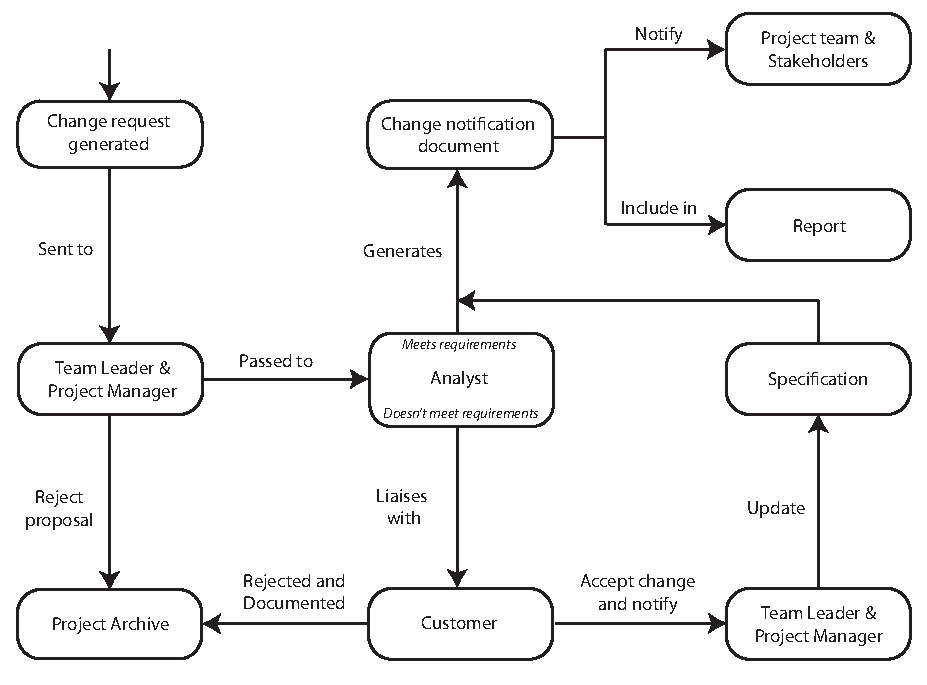
\includegraphics[height=33em]{res/change_management_diagram}
	\label{fig:change_management}
	\caption{Change management workflow}
\end{figure*}

In the end no change requests were submitted by any stakeholder not a part of the development team.
However, it is believed that this well documented and rigorous change management workflow would
have enabled the project to deal with any such change requests in an efficient manner.
Many minor changes, such as bug fixes, were discussed more informally within the development as
they had no effect on the schedule or requirements. This worked effectively whereas using the
formal change management procedure for such small changes would be overkill and lead to a lot
of time being wasted in communications overhead.

% Major changes? E.g. scaling back the goals to get a finished product.

A formalised change management workflow is necessary for a successful project, but it must only
be used where appropriate to ensure that it does not get in the way of smaller changes that
can be dealt with more informally.

\section{Stakeholders and Communication Plan}
\label{section:communication}

The various parties identified as stakeholders are shown in table \ref{tab:stakeholders} below. The relationship between the stakeholder and the project is shown, along with a rough estimate of their power and interest.\sidenote[][-2em]{See \bibentry{mendelow1991stakeholder}} This grid will form a reference for making sure that all interested parties are communicated with appropriately throughout the duration of the project.

\vspace{1em}

\begin{table*}
	\small
	\renewcommand{\arraystretch}{1.6}
	\begin{tabular}{p{9em} p{5em} p{2.5em} p{2.5em} p{9em} p{9em} p{8em}}
		\toprule
		\emph{Stakeholder} & \emph{Relationship} & \emph{Power} & \emph{Interest} & \emph{Requirements} & \emph{Measurements} & \emph{Communication Strategy} \\
		\midrule
		
		Project Team & Internal & High & High & 
		Good working environment, creative input. & 
		Meeting project spec, good grades! & 
		Various, detailed elsewhere. \\
		
		Supervisor --- Sara Kalvala & Internal & High & High & 
		requirement & 
		Adherence to spec, good PM, high quality write-up. & 
		Weekly meetings. \\
		
		Client --- Matt Leeke & Core \mbox{External} & High & High & 
		requirement & 
		measurement & 
		Weekly meetings. \\
		
		Second Assessor & Core \mbox{External} & High & Low & 
		requirement & 
		measurement & 
		Deliverables only. \\
		
		Projects Organiser --- Steve Matthews & External & High & Low & 
		requirement & 
		measurement & 
		Email or meeting if required. \\
		
		Playtesters & External & Low & High & 
		requirement & 
		measurement & 
		Email. \\
		
		Other future users & Rest of World & Low & High & 
		requirement & 
		measurement & 
		Website, forums, blog. \\
		
		The Haskell and FP Communities & Rest of World & Low & High & 
		requirement & 
		measurement & 
		Online as above, and via the final report. \\
		\bottomrule
	\end{tabular}
	\vspace{1.5em}
	\caption{Stakeholders for the project.}
	\label{tab:stakeholders}
\end{table*}

\noindent Communication within the project team is examined in detail elsewhere in this document, so the remainder of this section is concerned with the other stakeholders.

\subsection{Supervisor Meetings}

Regular communication with the project supervisor is likely to be a critical factor in success of the project. For this reason a weekly meeting with at least one member of the group if not more will be high priority.

\subsection{Client Meetings}

The client is clearly vital to the success of the project, and continual feedback on each release will allow for early identification of any problems. At least one meeting per release (ie each week) will be required, as well as further meetings and correspondence as needed.

\subsection{Projects Organiser and Second Assessor}

The projects organiser could exert a strong influence over the project if they wished, but as there are many projects and it would be inappropriate for them to demonstrate partiality, extended levels of communication are unlikely to be necessary. Brief updates pertaining to deliverables is all that should be required. But if the project organiser initiates communication then they should be made a high priority.

Communication with the second accessor is, for the most part, not appropriate, excepting when within the remit of the deliverables, i.e. the report and presentation themselves.

\subsection{Playtesters and End Users}

\subsection{The Haskell and Functional Programming Communities}

The overall end goal of the project is not just a game, but an examination of Haskell and Functional Programming as a game development environment. 



\section{Team Structure}

Before starting the development phase of the project the roles and responsibilities for
each team member were formalised. Each person was given a set of roles and responsiblities
for which they would be primarily in charge of. It was envisaged that these roles would
be flexible and that responsibilities would be shared, but having a formal specification
of the member ultimately responsible for an aspect of the project's development and management
would be useful for ensuring that everything was done correctly. The roles that were given
to each team member as laid out in the specification are as follows.

\subsection{Laith Alissa}
\begin{description}
    \item[Project Manager] Responsible for overseeing the human aspects of the project in general, including managing a schedule, organising meetings and collaborative development sessions. Makes decisions involving tradeoffs between project time, cost, and quality.
    \item[Customer Liaison] Meets with the customer at regular intervals to discuss the project progress, outlook, and any issues which are require customer input. 
    \item[Analyst] Responsible for ensuring the customer requirements are addressed during planning and development stages of the project, and ensures that the solution will sufficiently address the customers needs.
    \item[User Manager] Responsible for communicating with play-testers and users. Finds end users to test the product in the later stages of development, and provides feedback to the project team. Prime responsibility is to identify issues which are not clearly visible from the project development perspective, but are more apparent to end users. 
    \item[Graphic Designer] Responsible for prototyping and developing graphical design elements, such as ship sprites, terrain, maps and user interface.   
\end{description}

\subsection{Jon Cave}
\begin{description}
    \item[Code Reviewer] Responsible for interpreting other developer's code, checking for logical inconsistencies and familiarising themselves with the project as a whole.
    \item[Chairman] Responsible for coordinating meetings, ensuring all issues are resolved or at the least discussed, and that all meeting participants have a chance to voice concerns and contributions.
    \item[Testing and Integration Officer] Ensures the code is thoroughly tested for bugs, and discovered bugs are flagged and dealt with in reasonable time. Responsible for managing integration testing to prevent bugs occurring on the master branch.
    \item[Security Officer] Checks for security flaws in the product, performs security evaluations (such as penetration testing and code review) to ensure the product is sufficiently secure.
\end{description}

\subsection{Joseph Siddall}
\begin{description}
    \item[Software Librarian] Ensures team completes documentation to a sufficient standard for long term maintenance. 
    \item[Line Manager] Oversees day to day development, intervenes if a developer is off track, ensuring minimal time is wasted perusing low priority work.
    \item[Testing and Integration Officer] Ensures the code is thoroughly tested for bugs, and discovered bugs are flagged and dealt with in reasonable time. Responsible for managing integration testing to prevent bugs occurring on the master branch.
\end{description}

\subsection{Victor Smith}
\begin{description}
    \item[Team Leader] Leads the project. Responsible for coordinating the project team, ensuring team members are working to the best of their ability, responsible for making decisions when the there is no clear solution to a particular problem.
    \item[Lead Developer] Responsible overall for technical areas of the project. Consults other developers when there is development difficulty, also responsible for directing programming style and technique.
    \item[Composer] Composes soundtrack for the game, and produces required sound effects, voice overs, soundscapes, and other related resources.
\end{description}

\subsection{Common Roles}

Some of the roles were shared by the whole project team. This is because all of the
team members were involved in day to day development and game play design.

\begin{description}
    \item[Programmer] Performs the day-to-day programming specified by the line manager.
    \item[Tester] Performs general code testing (e.g.\ unit tests, component tests).
    \item[Gameplay Designer] Critically analyse gameplay design and experience, giving feedback to the team leader on how to improve the game's appeal.
\end{description}

\section{Risk Management}
\label{section:risk}
 
A proactive approach to risk management was taken. This technique was chosen in order
to maximise the probability of avoiding risks instead of having to move into `fire-fighting mode'
if something went wrong.\citepage{pressman2010}{page 745}
 
As part of this proactive risk management strategy, a number of potential risks were identified.
These risks are shown in table~\ref{tab:risks} along with their estimated probabilities of occurring
and impact if they were to occur.
 
\begin{table*}
	\small
	\begin{tabular}{l p{\textwidth / 2} l l}
		\toprule
		\emph{Risk} & \emph{Description} & \emph{Probability} & \emph{Impact} \\
		\midrule
		Length underestimate & The time required to develop the software is underestimated & Medium & High \\
		Team member illness & One or more team members unable to work due to illness & Medium & High \\
		Hardware failure & Damage to critical hardware causing loss of data & Medium & Medium \\
		Size underestimate & The size of the deliverable has been underestimated & Medium & Medium \\
		Requirements change & Large number of changes to requirements during development & Low & Medium \\
		Ambiguous requirements & Requirements are not fully understood or misinterpreted leading to
			loss of development time as the specification is recreated & Low & Medium \\
		\bottomrule
	\end{tabular}
	\vspace{1.5em}
	\caption{Risk identification and analysis.}
	\label{tab:risks}
\end{table*}
 
With the risks identified, and their likelihood and consequences estimated it is necessary
to draw up plans to mitigate their effects. There are three types of management strategies 
for individual risks: avoidance strategies to reduce the probability of the risk occurring;
minimisation strategies to reduce the impact of the risk; and contingency plans to deal with
the risk if it does arise.\citepage{sommerville2011}{page 601} It is best to avoid the risk,
but if this is not possible then minimisation of the effects and, finally, contingency plans
should reduce the overall impact of a risk on the project. The mitigation and management
strategies for each risk previously identified are listed in table~\ref{tab:rmm}.
 
\begin{table*}
	\small
	\begin{tabular}{l p{37em}}
		\toprule
		\emph{Risk} & \emph{Mitigation / Management} \\
		\midrule
		Length underestimate & Detailed work breakdown with weekly releases to ensure that
			schedule slippage can be caught early \\
		Team member illness & Well documented code (enforced by the software librarian) so
			that other members can quickly start work on less familiar sections of
			the codebase \\
		Hardware failure & Backups and distributed source control, see section~\ref{section:tools} \\
		Size underestimate & Detailed work breakdown structure \\
		Requirements change & Thorough change management system, see section~\ref{section:control} \\
		Ambiguous requirements & Thorough planning phase \\
		\bottomrule
	\end{tabular}
	\vspace{1.5em}
	\caption{Risk mitigation and management.}
	\label{tab:rmm}
\end{table*}
 
The final stage of the risk management process is monitoring. Throughout the duration of
the project each identified risk was reassessed for changes to its probability and
impact. This allowed the mitigation and management strategies to be revisited to ensure that
they were as effective as possible.
 
The two previously identified risks that actually occurred were team member illness and length underestimate.
On a couple of occasions a team member was ill and unable to attend group work sessions or work to their full
capacity. Fortunately, the team was able to reduce the impact of this by ensuring that the work each individual
was performing was not hindered by an absence. This was done by allocating work tasks to be as separate as
possible to allow more parallel development to occur. Also, an illness was never so severe as to stop a team
member from working for longer than a day or two. However, the issue of length underestimation was more serious.
 
% Length underestimation
%
% 1. More time required for network and GUI than hoped
% 2. (1) slowed the development of the ideal game
% 3. (1) was very informative for our goal of investigation of Haskell for game development
 
The proactive approach to risk management was a good choice. By reviewing the potential
risks before starting the development phase of the project it was much easier to avoid risks that could
have had disastrous consequences for the project. For example, by implementing a thorough backup strategy
prior to any data loss actually taking place it was ensured that no work would have been lost if a hardware
failure had occurred. Continuously monitoring and reassessing these risks was also helpful in preventing
any risks becoming more probable or having a greater impact.

\section{Legal, Ethical, and Social Issues}
\label{sec:legal}

Prior to embarking on this project several potential professional issues were identified
and discussed to ensure that they were addressed appropriately.

Any software project faces issues surrounding copyright and intellectual property. During
development the team were aware that all third party libraries used in the project must
be licensed appropriately. This meant only using software with a permissive license (e.g.
Apache, BSD, or MIT licenses) and no unlicensed proprietary software. It was also important
to avoid infringing on the intellectual property of established game publishers and their
existing games. Obviously it was infeasible to review all previously published games to
check if Serenity bears great similarities to any of them. However, the project team was
careful not to directly copy any designs or unique game play characteristics of existing
games that they are familiar with.

The games industry is faced with several ethical and social issues that were thought about
carefully when designing the Serenity game. Highly controversial issues that surrounds
current games, such as racism and violence, were thought about carefully and it was ensured
that they would not be issues with the Serenity game. This is because the game is based
in a fictional world with a very unrealistic graphical representation. Another social
dilemma for game creators to consider is that of the addictiveness of their creations.
Players often invest many hours, often consecutively, in playing games and can even spend
large sums of money on pay-to-play games. The game that was developed was designed to
have short playing periods that would allow convenient times for the player to quit.

\section{Evaluation of Tools and Techniques}
\label{sec:tools}

A number of different tools were used in the day to day running of the project.
These tools were used to ease the collaboration between members by ensuring that everyone knew
what they were supposed to be doing and how to share it with the others.

\subsection{Source Control: Git}

Source control systems are an essential tool for software projects, especially those
with multiple developers. Using source control to easily track the changes to source
code is helpful because, as McConnell explains, having a history of changes helps a
developer to identify the origin of bugs quickly.\citepage{mcconnell2004}{page 667}

The Git source control system\sidenote{\url{http://git-scm.com/}} was chosen for this project.
Git was chosen for a number of reasons. Firstly, it has a lightweight branching model which
allows for quick creation of new development branches for experimental features independent of
any other development. Chacon notes this as Git's ``killer feature''.\citepage{chacon2009}{page 38}
Another reason for choosing Git is its distributed nature. Every user has a full clone of the
entire repository that can act as a replacement for any other instance of the repository; this means
that there is no single, centralised point of failure.

A centralised master repository was hosted on Github, a popular code host.\sidenote{\url{https://github.com/}}
This made it easier for team members to share their changes to the code base. Once a change has been made
it can be `pushed' to the Github repository; other team members can then `pull' it to their local
repositories.

Git was an ideal source control system for the project. Not only does it allow the users to see
the entire history of changes made to the project it makes collaborative development between
multiple team members incredibly easy. Instead of having to resolve conflicting changes to files
it is possible to use the built in merge tool to combine the work of two or more people on the
same set of files with minimal effort. Git is recommended for all future development projects.

\subsection{Tracking and Managing Releases: Trello}

\begin{marginfigure}
	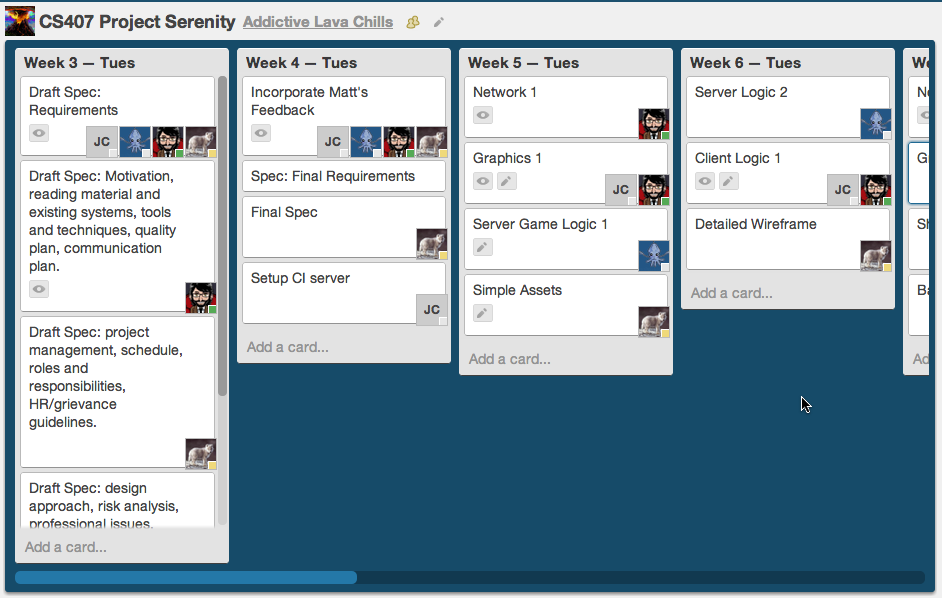
\includegraphics[width=6cm]{res/trello.png}
	\caption[Trello]{Project Serenity's Trello page}
	\label{fig:trello}
\end{marginfigure}

Trello is a modern, online take of an age old concept --- a wall of post-its. Trello allows for overall planning of tasks and communication between members in a highly dynamic, fluid way. Cards are arranged into a list-of lists, each list being some kind of functional decomposition or `stovepipe'. Trello has been used in the project to track the requirements for each weeks releases, but still allowing rapid changes to be made and communicated.

Trello acted as a useful reference to the current state of the project: what tasks are planned and who is doing them.
It is a good tool for keeping a small group of people organised, but requires careful management to keep it
up to date and useful.

\subsection{Bug Tracking: Github Issues}

Trello does not entirely alleviate the need for a full bug tracker. When working of development of
individual features and components it was necessary to have a method of tracking more transient issues
and tasks. The initial plan was to use the service provided by Fogbugz, a stand alone bug tracking
web application. However, in the end the Issues feature built into Github hosted repositories was
used. This was decided because it reduced the number of third party services that were relied upon
and it provided better integration with the hosted repository itself. Although it is much more minimal
than Fogbuz, it provided enough features, such as milestones, labels, email notifications, and
issue assignment, for this project.

An issue tracker was very useful for noting down smaller tasks and bugs that cannot be fixed immediately,
but must not be accidentally forgotten about. If a project is using Github to host code then the
Issues component is recommended if only simple issue tracking features are required. However, for
more complex requirements a more fully featured service may be a better option.

\subsection{Backups}

Backups of the source code and other project assets are essential. In the event of a
disaster, such as losing a computer to a fire, it must be possible to recreate the
entire project in its latest state quickly and without any repetition of work.\citepage{mcconnell2004}{page 669}
The use of Git and Github for source control made it simple to ensure that all
source code was located on multiple computers. By `pushing' commits to the Github
repository all code was stored in the cloud. When other team members `pulled' the code
later on it was then mirrored on their computers as well. Extra precautions were taken
by also `pushing' the Git repository to private servers owned by the team members.
Also, the free service provided by Dropbox\sidenote{\url{https://www.dropbox.com/}}
was used to share and backup any other files, such as assets and planning notes.

Fortunately a situation which required recovery from backups was never encountered,
but the strategies put it place should have been more than adequate if the need ever
arises in the future. Since the main backup strategy was part of normal development
workflow it was impossible to forget to implement it. However, it does have to be ensured that
all members are sharing their changes as frequently as possible (even if a feature is
not fully finished) to prevent any work in progress from being lost in case an individual's
computer dies. The extension to this core backup strategy, storing the repositories
on other personal servers, was easy because of Git's feature set which was designed
to be distributed in nature and so allows tracking and updating of multiple remote repositories.

\subsection{Continuous Integration: Jenkins}

Section~\ref{sec:testing} introduced the idea of continuous integration as a method
of regularly running the test suite and performing a full build of the software.
The Jenkins continuous integration server\sidenote{\url{http://jenkins-ci.org/}}
was used for this project. Jenkins was chosen because it is a widely used open
source project.\sidenote{\url{http://stats.jenkins-ci.org/jenkins-stats/}}
Jenkins also works well with projects hosted on Github because of its Github plugin\sidenote{\url{https://wiki.jenkins-ci.org/display/JENKINS/GitHub+Plugin}}
and Github's Jenkins specific post-receive hook.

Although Jenkins does not have a very good user interface it suited the needs of
this project. It was a good tool for running a test suite with every change to the
code base and ensuring that the game would build correctly. Email notifications on failure
were useful, but also relatively noisy at times. Continuous integration is probably
more useful for more mature projects that need to ensure that changes do not introduce
any regressions than it is for a project in the early stages of development when a lot
of features are not fully working.

\chapter[Requirements]{Functional and Non-Functional Requirements}
\label{ch:requirements}

\chapterepigraph{``All things are created twice; first mentally; then physically.  The key to creativity is to begin with the end in mind, with a vision and a blue print of the desired result."}{ Stephen Covey}

\newthought{Starting a sentence} with a new thought.


% help site at http://www.projectmanagementhelp.com/how-to-write-functional-requirements/
% bullet point these requirements, describe them, specify any details.
% include bain quite as footnote
\section{Functional Requirements}




\section{Non-Functional Requirements}


functional - 2d, realtime strategy, multiplayer, ship design, resource system, ai, planetary capture resource system, possiblity of campaign style multiplayer, tactical zoom/gameplay, fow, hw requirements, haskell.
non-functional - fun, reliable, secure, short lived game sessions, 

\section{Evaluating the Success of the Project}

Project success depends highly upon perspective, one stakeholder might consider the project beyond successful whereas another stakeholder may consider the project a total failure. Evaluating success must consider a variety of perspectives, and even then it may not be as simple as a yes or no answer. 

\begin{quote}
An architect may consider success in terms of aesthetic appearance, an engineer in terms of technical competence, an accountant in terms of dollars spent under budget, a human resources manager in terms of employee satisfaction, and chief executive officers rate their success in the stock market.
%todo reference Freeman and Beale (1992,p. 8) 
\end{quote}

%todo: this is vics stuff, didn't even proof it, shot-not (Laith),
\paragraph{Shenhar et al, 1997} \cite{shenhar} In this paper it is suggested that the traditional measures of project success --- namely time cost and quality --- are perhaps not the best, and points out the disagreement in the literature on this area. Building on evidence from previous studies, the authors suggest a new, multidimensional, framework for project success; and, notably, back this up and expand upon it by utilising empirical evidence.

This evidence takes the form of 127 structured questionnaires, returned from project managers from a variety of industries.\sidenote[][-6em]{It is claimed in the paper that despite this selection having not been made at random, with no consideration to stratification, and that 'the end products were aimed at a military market', that there is not an inherent bias. Especially in light of the low sample size this should be considered to be a somewhat dubious claim.} This data was then analysed using numerical measures from previous work\sidenote[][1em]{Specifically Cooper and Kleinschmidt, 1987;  Pinto and Stevin, 1988; Stuckenbruck, 1986; and Dvir and Shenhar 1992. (See full bibliography).} and the dimensionality of results determined using factor analysis.\sidenote[][1em]{Factor analysis being a statistical technique to determine the underlying dimensionality of a data set without previous knowledge of it. See Brayant and Yarnold (detail in bibliography) for a full treatment.}

Despite an initial hypothesis of three dimensions to project success, the analysis suggests that there are in fact four. These dimensions were then correlated(using Pearson's Correlation) with the overall assessment of project success, with favourable results; and the relative strength of each measured, both for projects in progress and completed projects. The strength was seen to be consistent, apart from the fourth dimension which was significantly better correlated in completed projects. This is the 'future potential' dimension. 

This empirical experiment causes this research to stand out in a way other papers on the subject of project success do not, in that the claims are in fact backed up. This is in sharp contrast to Atkinson's paper (see below).

Another notable feature of this paper is that in addition to the scientific numerical approach, a significant percentage of the text is given to practical consequences of the results and implications for the practitioner. Given that it is now nearly fifteen years old it is surprising that these ideas do not feature more prominently in project management canon.
%
%In the paper ``Project management: cost, time and quality, two best guesses and a phenomenon, its time to accept other success criteria'' %todo citation
%, Atkinson considers typical assessment criteria to be insufficient, and proposes a new method known as "The Iron Triangle" which aggregates many existing paradigms to form a new way of evaluating project success.
%
%In the paper ``Mapping the dimensions of project success'' Shenhar et. al. identify four dimensions which measure the success of a project, and can be further used to quantify the success of a project against a benchmark of well known projects throughout history.
%


The Iron Triangle is a primitive tool for measuring the balance between time, cost and quality. It has no quantifiable properties and is mainly an illustrative tool, but it does somewhat accurately express the relation between the three constraints.
\begin{marginfigure}
	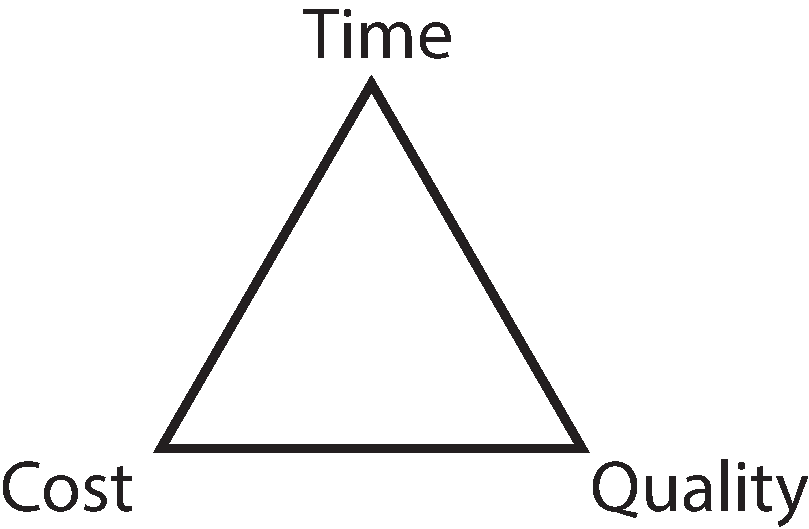
\includegraphics[width=55mm]{res/pm/TCQ_triangle}
	\label{fig:TCQ_triangle}
	\caption{The Iron Triangle}
\end{marginfigure}
Selecting two of the properties as desirable will be costly to the third, for example demanding a high quality product in little time will escalate the cost. The project had no real notion of monetary cost, so the balance was largely between quality, project time and personal time, where the personal cost a team members marks from other assignments, time for hobbies, sleep, etc. For almost all project components there would be an imbalance between the three properties, and most often, the \emph{personal time} property would need to be increased to ensure good quality products while keeping to schedule.  


\paragraph{Success Dimension 1 : Project Efficiency}
The first dimension is interesting in the way it applies to software projects, since efficiency is extremely difficult to guage. Unlike a task requiring manual labour, efficiency can be assessed fairly easily since most tasks are repeatable and hence can be modelled fairly easily. It's difficult, on the other hand, to compare two software projects, since not only are they very rarely alike, but efficiency is not easily quantifiable. Some managers try to quantify development progress by measuring lines of code per day, as Hertzfeld implied in his article ``-2000 lines of code'', the number of lines a developer has written per day may have no bearing on the work accomplished. Even it there was a convenient function of project progress to mark efficiency, that efficiency would likely be subject to changes. Suppose a large software project launches, stays on schedule and outputs an excellent number of lines per day, it might be the case that the developers are taking shortcuts and not being prudent, which could cause a massive slump in the efficiency late down the line when it's discovered that the initial few milestones are bug ridden and need to be revised. By contrast a project team missing the initial deadlines might be investing a large amount of thought into their work which could accelerate their efficiency later down the line. The important thing to note is that efficiency hinges on perspective, and it's very difficult to find a function to assess the efficiency of a software project.
%%todo: Sounds sloppy so far, revise!
Given that it is in fact necessary for the model, it would be wisest to measure efficiency by comparing each estimated milestone completion date with it's actual completion date, since the milestones were all met on time, but some features were lacking, it's fair to claim the project progress was reasonably efficient \emph{efficiency} available. 

\paragraph{Success Dimension 2 : Impact on customer}
%todo: Matt's feedback?

\paragraph{Success Dimension 3 : Business and Direct Success}
Business and Direct success is a measure of whether the project provided ``the sales, income, and profits as expected'', ``increase[d] business results'' or whether the project ``helped to increase market share'' \cite{shenhar}. Shenhar does elaborate that other projects may not fall under the same assessment criteria, but will have some mechanism of measuring direct success. Since this project is academically motivated rather than monetarily driven, it would be fair to assess the success outcomes the requirements discussed in section \ref{sec:reviewrequirements}. The project met most of these requirements, and the requirements it failed to meet were considered the least important. The project was largely successful in creating a fun game in Haskell, which met almost all the functional requirements and fulfilled all the non-functional requirements, granting the project at least a partial success under Dimension 3.
 
\paragraph{Success Dimension 4 : Preparing for the Future}
The fourth dimension investigates how prudent the project is, whether it has invested in future opportunities, whether it explored further ideas, innovations or skills which may be required in the future. Assessment under this dimension can only result in an overwhelming success. The project explored two concepts which are already hugely popular and only growing in popularity, namely indie games and the Haskell programming language. Haskell's growing popularity is undeniable, it's a concise yet extremely powerful language which has recently being adopted by an increasing number of companies including ABN AMRO, Anygma, Amgen, Bluespec and Eaton. It has been used to construct many large scale projects such as ASIC, FPGA (design software), Haskore, GHC, Darcs and HAppS, projects which are of comparable size and complexity of many corporately produced games. \cite{realworldhaskell}

%todo: Probably won't be able to phrase of cite this bit properly tonight
Game development is also a very rapidly growing market, with the advent of mobile devices the target audience for video games barely excludes any social group.  
% Can't think of how to finish this
The project has produced a wealth of experience for developing games in Haskell...

\paragraph{Overall Success}
Each dimension is a measure of success for a time frame, the first being concerned with the immediate results of the project, the fourth being concerned with the distant future and the interactions the project may be a part of in the future. This project was by no means perfect, but it showed strong signs of success when applying Shenhar's success measurement criteria.


\section{Conclusions}

\begin{itemize}
\item Assessment of our key decisions
\item Conclusions on Haskell
\end{itemize}


\chapter[Overall Conclusions]{Overall Conclusions}
\label{ch:conclusions}
%\containsfigures{Summary of Conclusions}
%\containslistings{Summary of Conclusions}
%\containstables{Summary of Conclusions}

\chapterepigraph{Haskell is an abstract research language used only in academia, education, banking, stock trading, circuit design, embedded systems, cryptography, operating systems research, bioinformatics, phone apps, and web services.}{Jafet, quoted in \emph{Haskell Weekly News} Issue 265}

\newthought{Much has been learnt over the course of this project}, but as always it is hard to crystallise the full advantage of personal experience into an widely accessible form. The importance of continued research into software design principles is clear: software continues to be a driving force for society and computer use is still increasing at a brisk pace,\cite{borodovsky2006marching} yet actually writing software remains difficult and error prone.\cite[1em]{paulk1993capability} 

This project aimed to show the paradigm of functional programming in action, and specifically the language Haskell. What was once considered merely a research language is now finding uses in many places in industry, and has an active and numerous online community. Haskell and FP remain outside of the mainstream, however, and education and encouragement will be required before these techniques can be widely taken advantage of. This project has attempted to contribute to this agenda by demonstrating that Haskell is effective in a field thought normally to be the preserve only of C++: that of game programming. 

In order to be sure this approach would be viable, various aspects of the method needed to be carefully considered, as detailed in Chapter~\ref{ch:rd}. The most important point to note here is that the game, \emph{Project Serenity}, was designed purely on the merit of being a good game that was achievable in the time frame, \emph{and that no considerations of what would best suit the language it was to be written in}. This is crucial to the conclusions that may now be drawn.

The details of developing Project Serenity --- as detailed in Chapters \ref{ch:game} and and \ref{ch:guide} --- have held some surprises, but the overall experience really has been like any other software project. Some problems were circumnavigated easily, others required some time and the invention of novel solutions. Some parts of the implementation, such as the AI framework and data model, very much suited the standard functional approach, whereas others, such as the GUI framework required some thought to code in a functional way. Advantages and disadvantages to Haskell were apparent, and have been discussed. But the main finding to be stressed is that the disadvantages were small: the difference between the classical problems `suited' to FP, and areas such as graphics and networking --- that people assume would be difficult or impossible --- are either small or non-existent. The hardest problems to be overcome during the project were instead from unexpected directions and generally not related to the functional paradigm itself, such as dependency problems with Cabal (see Section~\ref{ssec:dephell}).

It is important to stress this point, and it can be seen as the most important point that this project has aimed to demonstrate. When talking about the project during the course of the development, the project team were asked frequently questions like `what parts of the implementation really suited Haskell / really didn't suit Haskell', or 'how has the game you have designed been made to really demonstrate FP'. The point is that the game was designed simply to be a good game, and the development was \emph{all} eminently doable with Haskell. Some areas were harder than others, but this would be the same in any language. If Project Serenity is to have demonstrated anything, it is that the advantages of FP really do exist (testability, maintainability, equational reasoning, etc) while most of the usually cited disadvantages (low performance, hard to understand, cannot handle IO well, even lack of library support) do not. It follows that the real barrier to entry to functional languages like Haskell is not a technical aspect of the language --- as often claimed --- but merely a lack of familiarity with the paradigm.

\section{The Importance of Design Patterns}

One of the main weapons brought to bear against software complexity is that of design patterns, and their importance as software development tools is well established.\sidenote{See, for example, the well renown software practice guide: \bibentry{martin2003agile}.} However, because FP can be so different from OO programming, different design patterns are required; or, alternatively, a different perspective on the \emph{same} underlying principles is required. Therefore, a big focus in the presentation of the results in this report, especially those in Chapter~\ref{ch:guide}, is on design patterns for the functional programmer. This focus is to enable functional techniques to be accessible to a wider audience than the usual academic style of research into these languages usually allows.

Many of the techniques used in Haskell programming --- such as use of Monads, Monoids, Arrows, etc --- has come about through mathematical results and reasoning. Category theory has, somewhat surprisingly, turned out to be a rich source of design patterns to be used in practical programming. While one does not need to know anything about category theory to actually make use of any of these results, many of the best Haskell techniques discovered in recent years (such as separation of concerns with free monads) are still underused because they are yet to be translated from mathematics into the language of software design patterns. One of the main reasons for this is, of course, that these developments are very new, and that currently techniques like these are being invented and refined at a very rapid pace. Research normally concentrates on one particular area or design pattern without bringing the full picture into view. It is for these reasons that this project has taken the relatively novel approach of ``development as research''.

\section{Development as Research}

The aspect of this project that makes it unusual, especially for a fourth year group project, is the two layered approach. There is the game itself, which as previously stated was designed independently of all other concerns. This part of the project was a software development project pure and simple, with a customer and a product delivered at the end. But interleaved with this was the primary concern of evaluating Haskell as a development language. The novel idea here is that the first part allows for greater value in the second --- value which isn't available in research that focuses only on a single use or pattern. 

As this is a new and largely unparalleled idea (See Section~\ref{sec:litRevDesigningGame}) the method is somewhat unrefined. Keeping track of the research concern while in active development can be difficult, and for this reason great care was taken to record problems or notable events during development. But it is likely that further improvements can be made if future projects of a similar nature are undertaken. It is possible, for example, that undertaking two implementations of a design simultaneously in different languages would yield further insights. 

\section{Limitations of the Project, and Recommendations for Future Work}

The main limitation of the project has been that, due to time constraints, the complete life cycle of the game could not be completed. The development schedule that was initially planned proved to be quite ambitious, as is often the case in such projects (see Chapter~\ref{ch:pm} for more details). This has meant that the extensive playtesting that was originally planned was not able to be completed, and some of the aspects of coding in Haskell (i.e. maintenance and reuse) have not been as thoroughly tested as they might have been. Despite this, it can be said that the time available was as well spent as could practically be expected.

Once the academic considerations of sharing work before it is marked are no longer relevant, it is planned to open source at least part if not all of the Project Serenity code. It is hoped that work on the game will continue and eventually finished. 

While the project does try and infer conclusions about functional programming in general, many of the conclusions can only be said to apply to Haskell itself. Future work could contrast and compare many different languages being used for similar projects, and what design patterns are similar and can apply more universally. For example, it has been suggested that continuation mechanisms in many languages can be used like the Haskell `do' notation to code monad expressions.\cite{piponi2008}

The content of Chapter~\ref{ch:guide} is an attempt at a `guide' to design patterns for Haskell programming, but much more work on this subject is possible, and indeed desirable. Free monads, lenses, arrows, functional reactive programming, etc, are all active development areas; but there is still a paucity of full guides on how to use these techniques in tandem in a large project. Indeed, a whole book on the subject would be possible.

If the advantages of Haskell and other functional languages are to be be as widely available as possible, routes to understanding them and using them from mainstream development are required. Much work could be done on comparing and contrasting functional from imperative design patterns. 

\section{Summary}

It has been demonstrated that developing a game fit for the current independent market is entirely feasible using the Haskell language. The game was designed purely on the merits of being a good game, not to be well suited to a functional implementation. None of the problems usually touted against the use of functional languages for such projects were encountered, including in areas requiring heavy use of IO, such as graphics and networking. A number of design patterns were found to be especially advantageous, details of which are to be found in Chapter~\ref{ch:guide}. 

There are many advantages to the use of functional languages, yet they are often not used for ill-founded reasons. This project has shown that Haskell is an extremely attractive language, and suggests that it should be taken seriously as an industry tool.



\appendix
\chapter[--- Monads and Other Fundamental Haskell Design Patterns]{--- Monads and Other Fundamental Haskell Design Patterns}
\label{app:monads}
%\containsfigures{Monads and Other Fundamental Haskell Design Patterns}
%\containslistings{Monads and Other Fundamental Haskell Design Patterns}
%\containstables{Monads and Other Fundamental Haskell Design Patterns}

\emph{This section could be dropped if there is no time to write it, and replaced by references to online tutorials.}

\section{Functors}

\section{Applicative Functors}

\section{Monads}

\section{Monad Transformers}

\section{Monoids}

\section{Category Theory}

\backmatter
\chapter{Acknowledgements}

LOL

\begin{fullwidth}

\def\bibname{Full Reference List and Selected Bibliography}
\nocite{*}
\bibliographystyle{plainnat}
\addcontentsline{toc}{chapter}{\bibname}
\bibliography{references}

\end{fullwidth}
\printindex

\end{document}
